\chapter{Chapter I}
\section{APEX}

\begin{enumerate}
\item Langkah pertama yang harus kita lakukan yaitu membuat apex dan memasukkan sebuah data ke dalamnya. Agar data bisa di kelola lebih mudah di bandingkan menggunakan Miscrosoft Excel. kita harus memasukkan data yang sudah ada. Contoh data yang akan saya masukkan ke dalam apex yaitu sebagai berikut:
    \begin{figure}[!htbp]
    \centering
    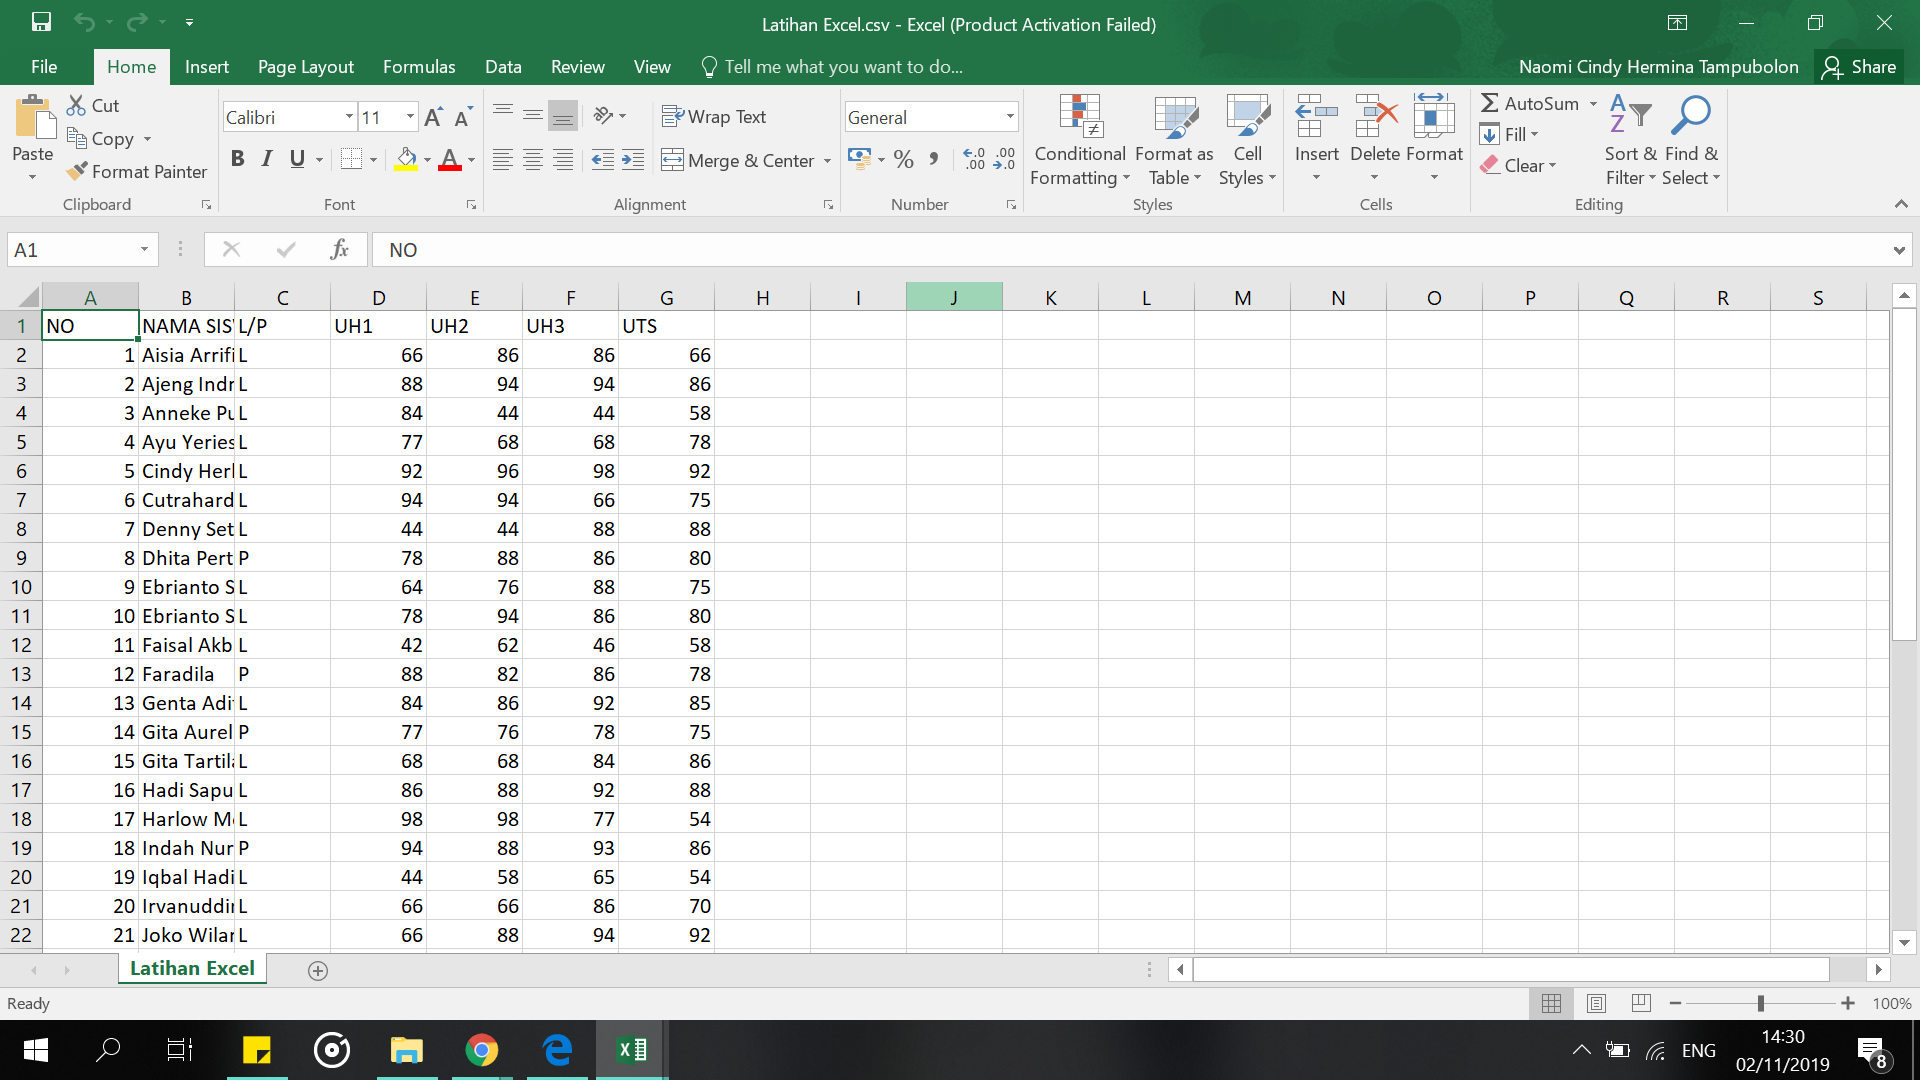
\includegraphics[width=9cm]{picture/01.png}
    \caption{Contoh Data}
    \end{figure}
    
\item Kemudian save data, Lalu Export dan ubah ekstensinya menjadi .csv, contoh sebagai berikut:
    \begin{figure}[!htbp]
    \centering
    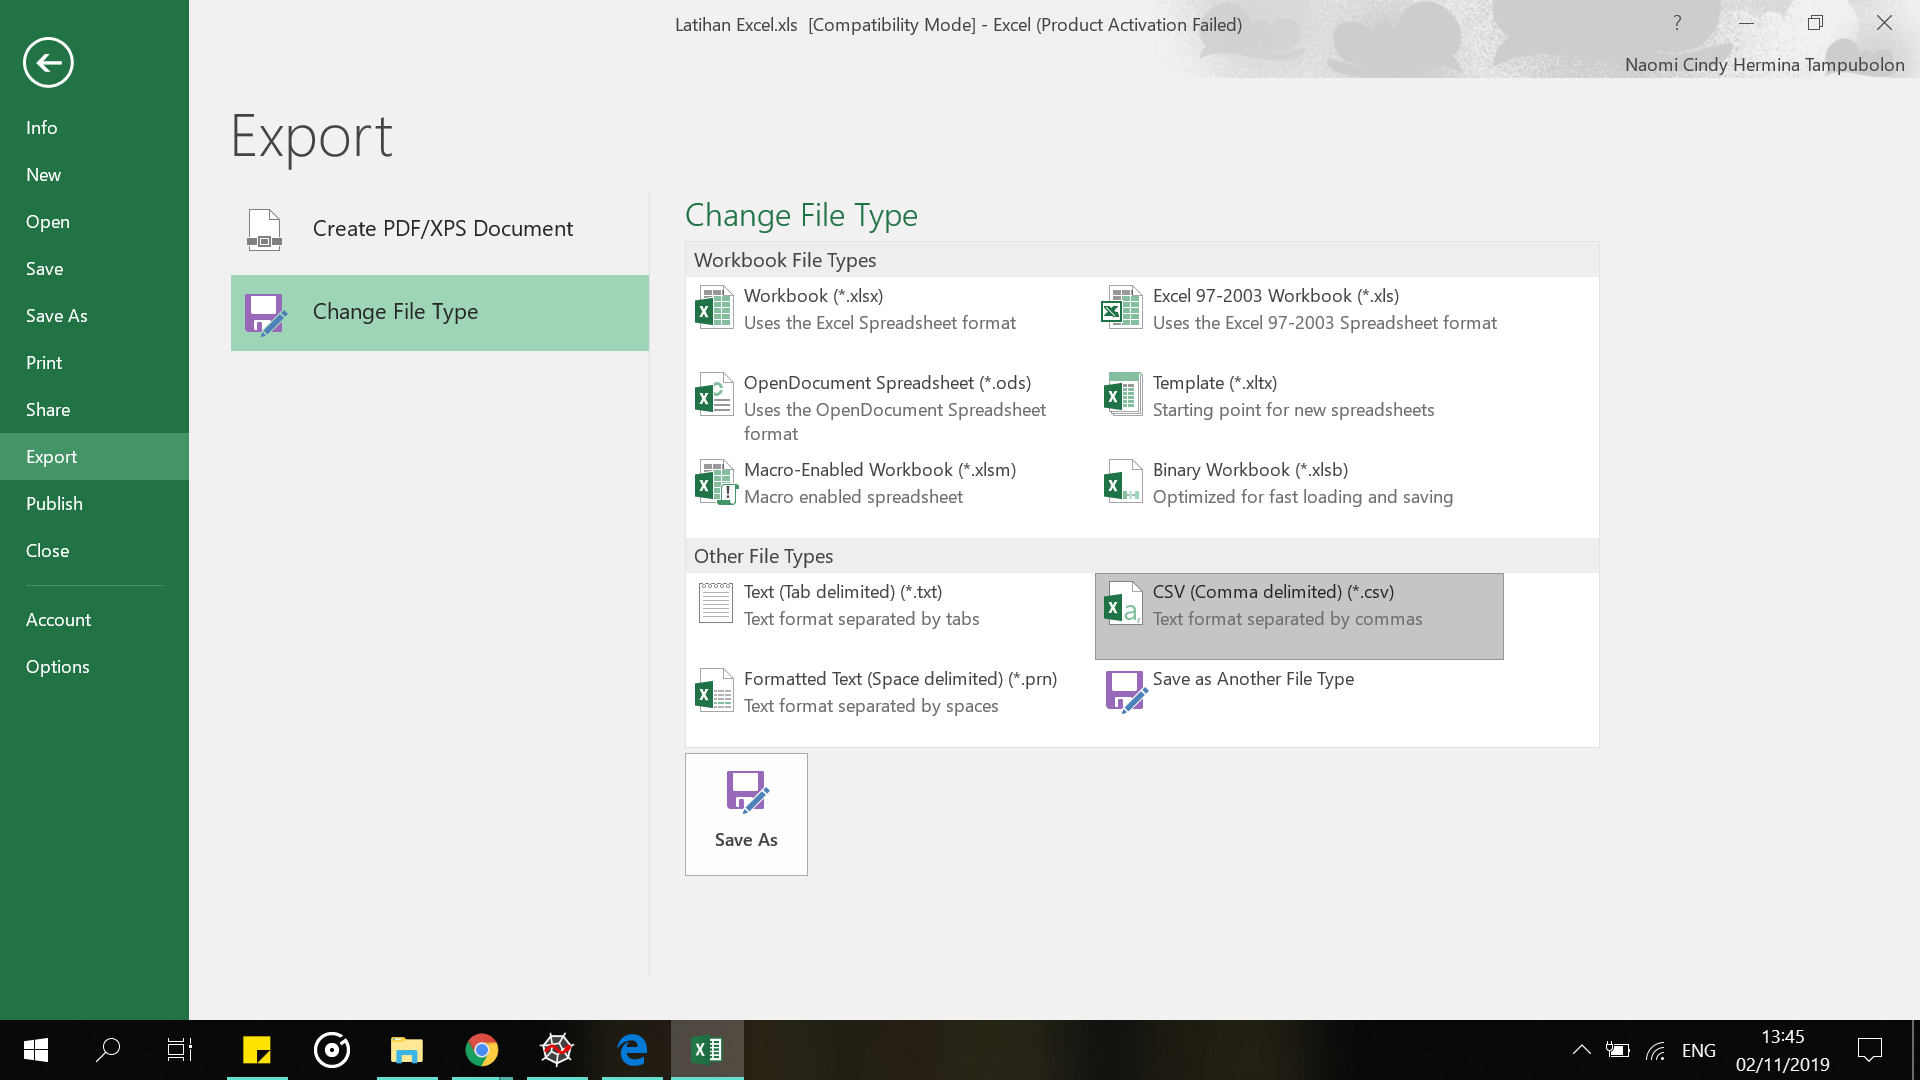
\includegraphics[width=9cm]{picture/02.png}
    \caption{Contoh Data}
    \end{figure}
    
\newpage
\item Buka link berikut: https://apex.oracle.com/en/ seperti gambar berikut:
    \begin{figure}[!htbp]
    \centering
    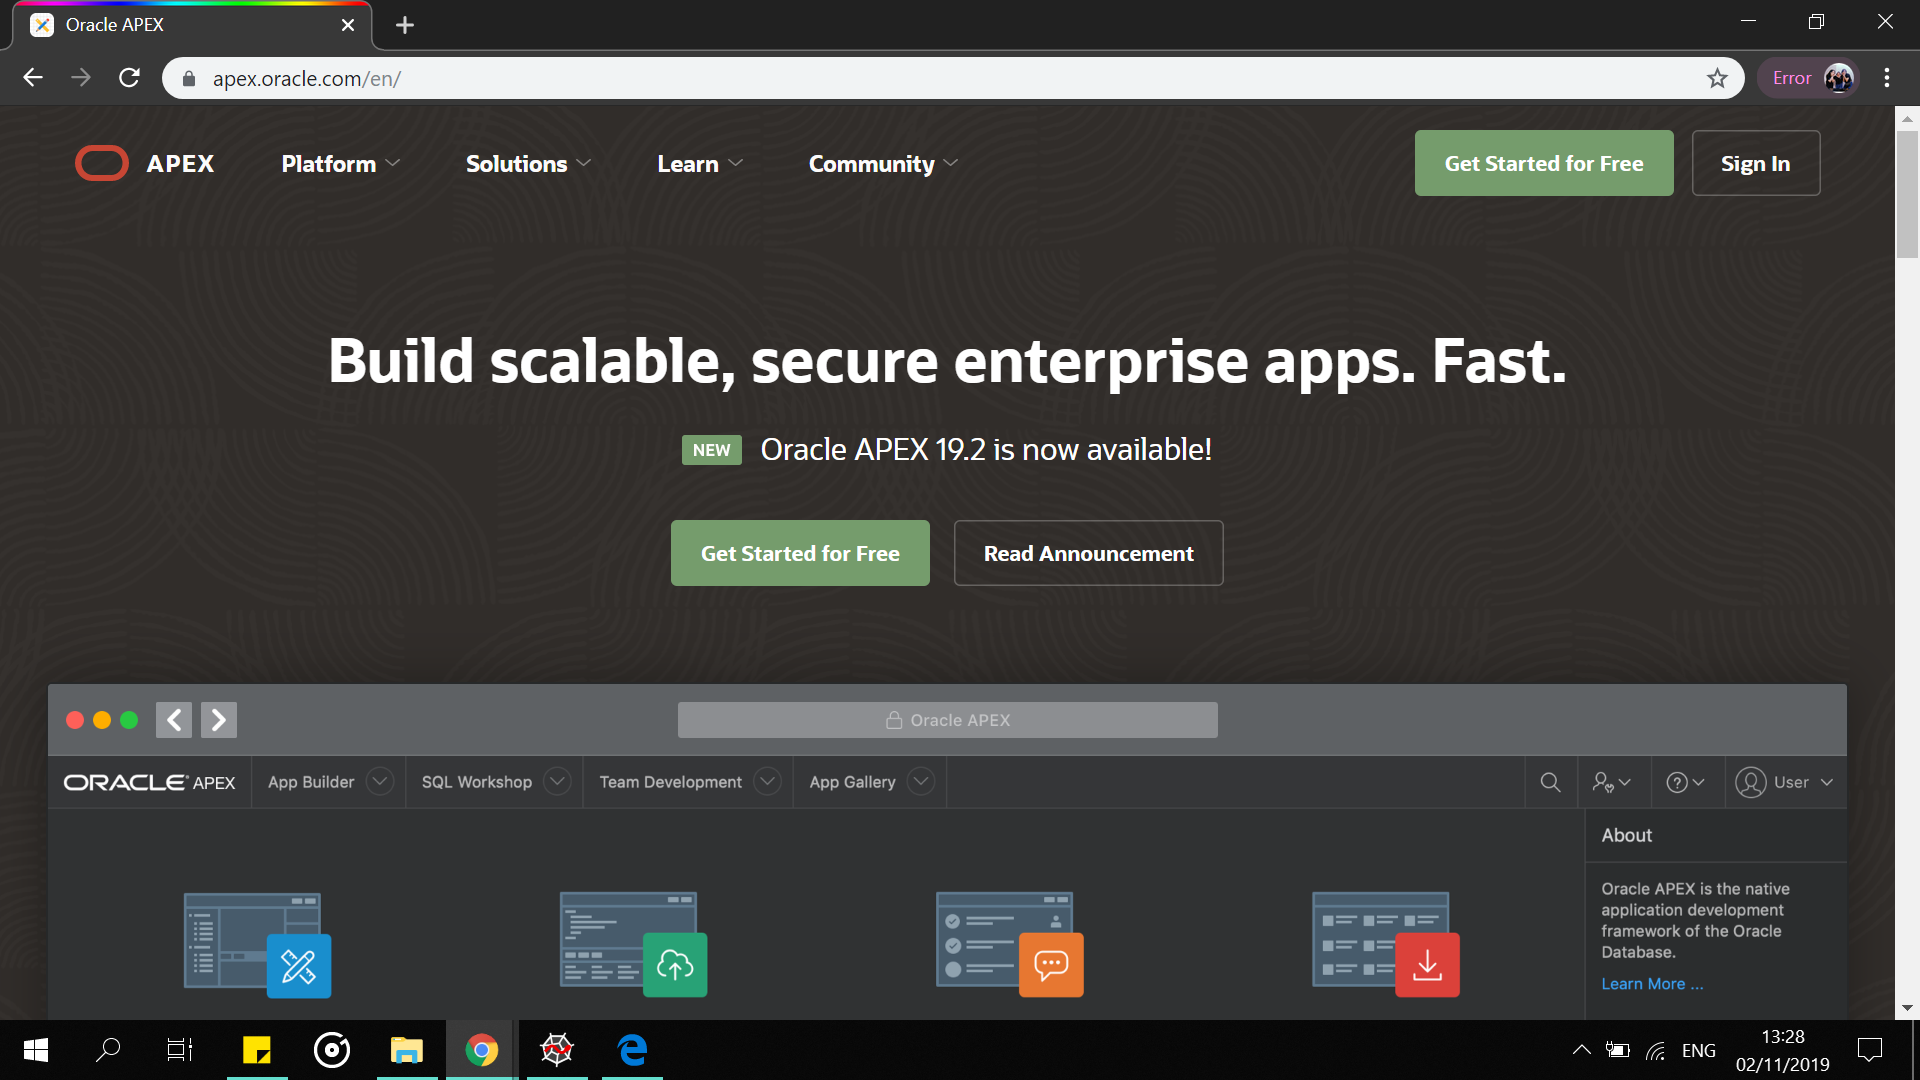
\includegraphics[width=8cm]{picture/03.png}
    \caption{Contoh Website yang dibuka}
    \end{figure}
    
\item Kemudian klik "Get Started for Free" lalu akan muncul seperti gambar berikut:
    \begin{figure}[!htbp]
    \centering
    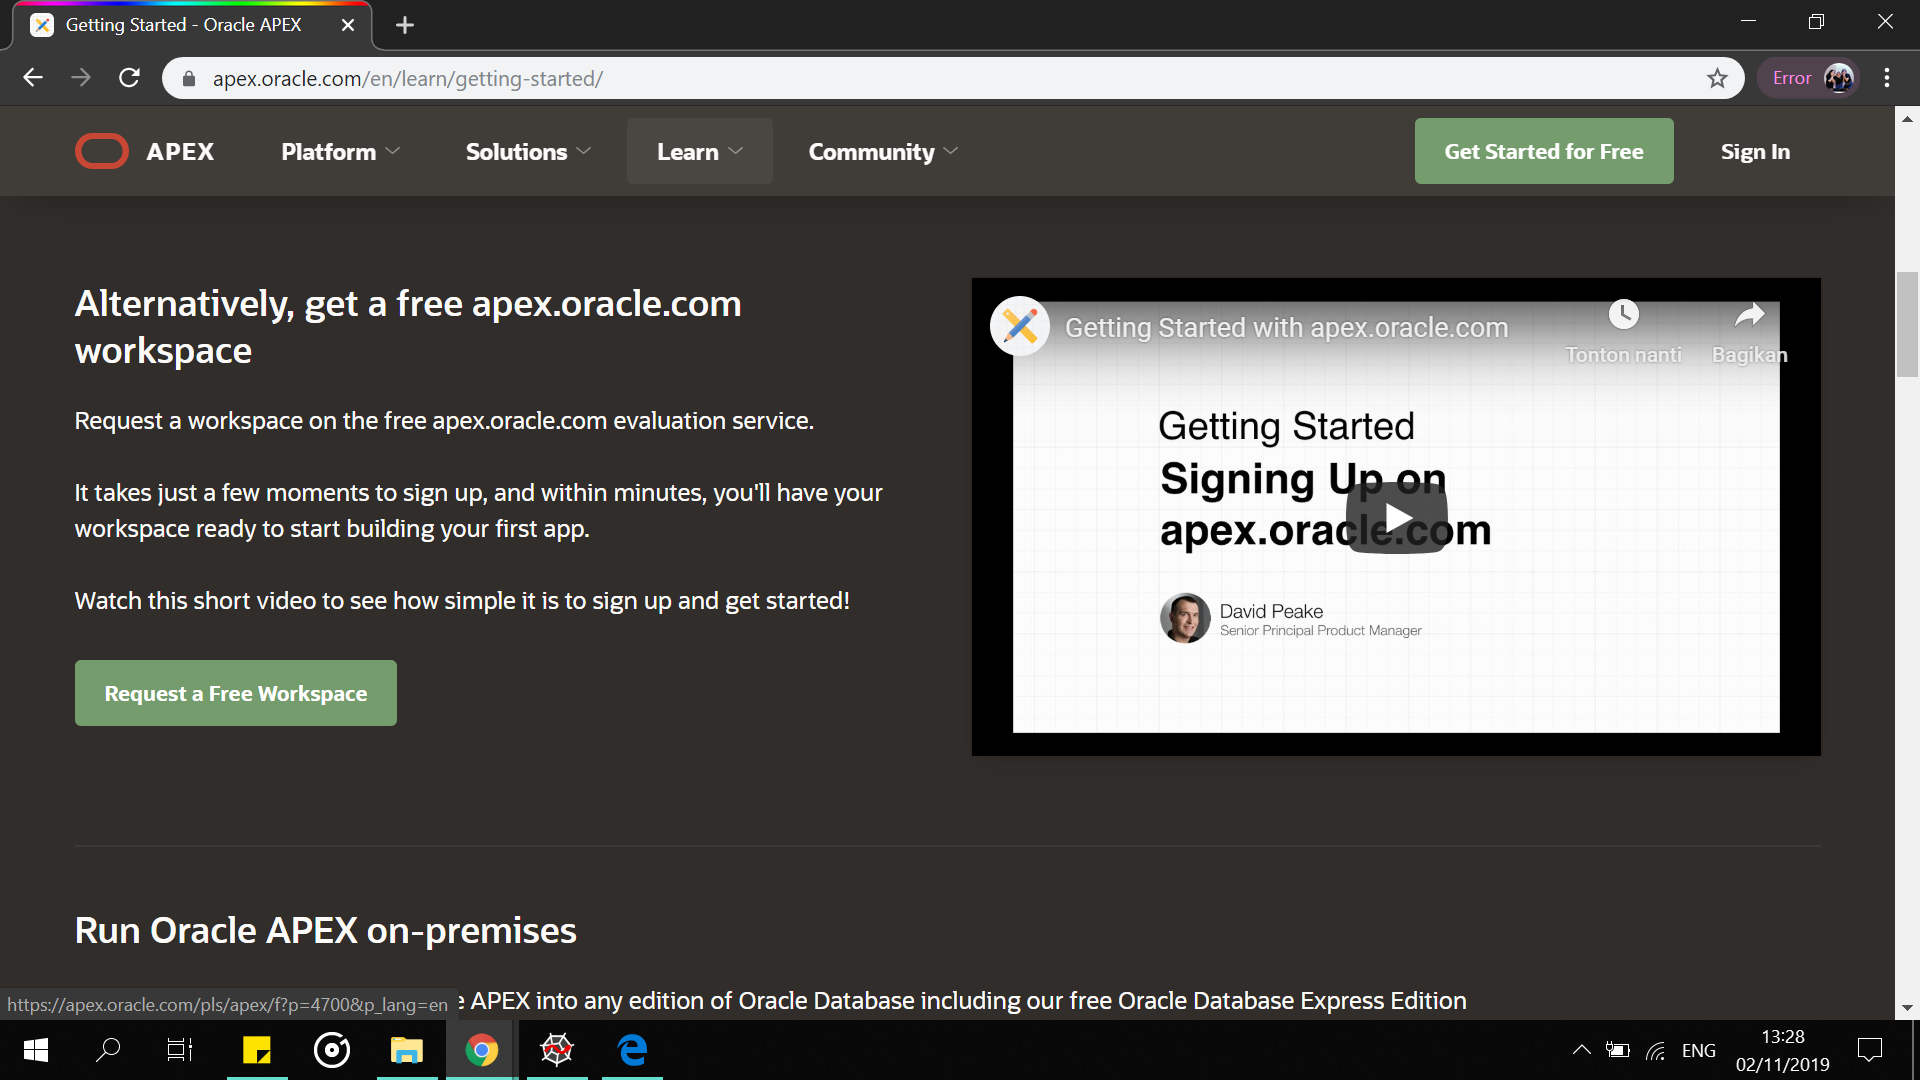
\includegraphics[width=8cm]{picture/04.png}
    \caption{Contoh Website yang dibuka}
    \end{figure}

\item Lalu akan muncul gambar sebagai berikut:
    \begin{figure}[!htbp]
    \centering
    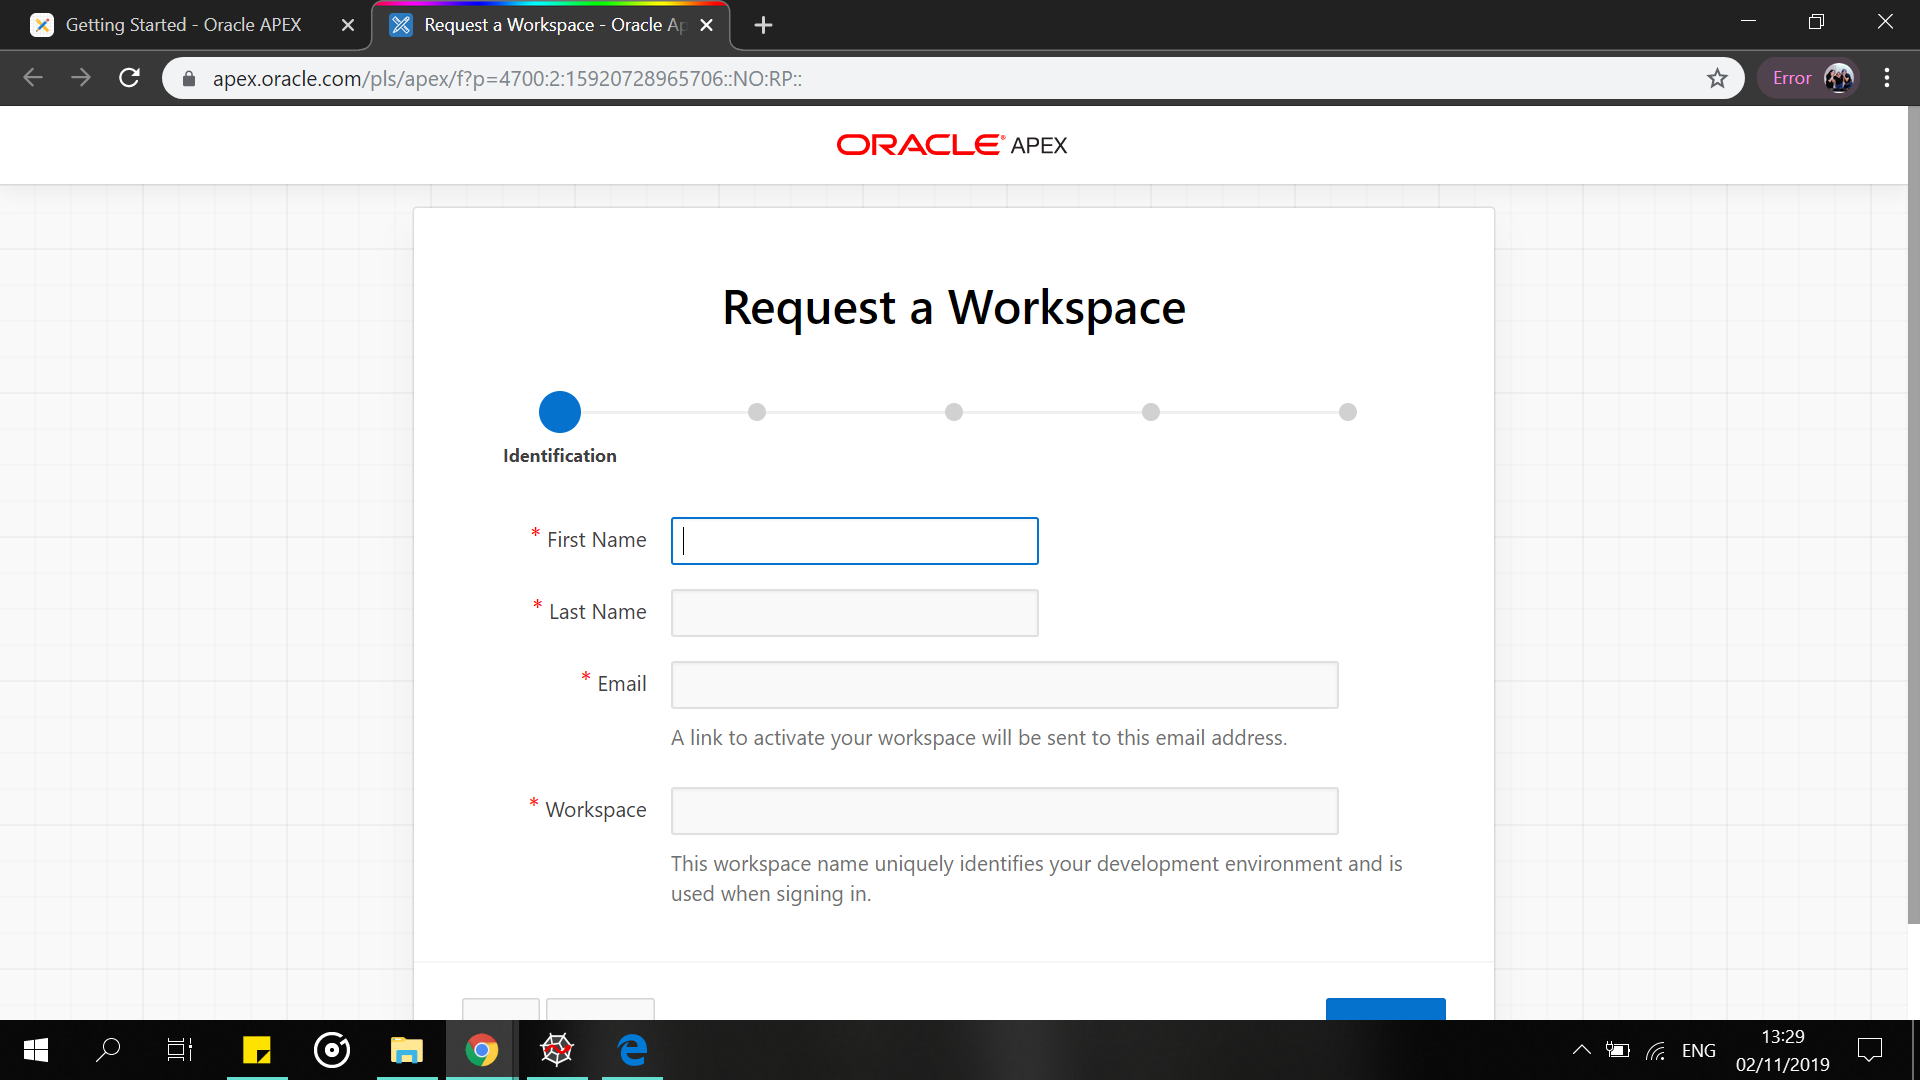
\includegraphics[width=8cm]{picture/05.png}
    \caption{Contoh Mengisi Form}
    \end{figure}
    
\newpage    
\item Lalu akan muncul isi form. Dan kemudian isi data datanya seperti berikut:
    \begin{figure}[!htbp]
    \centering
    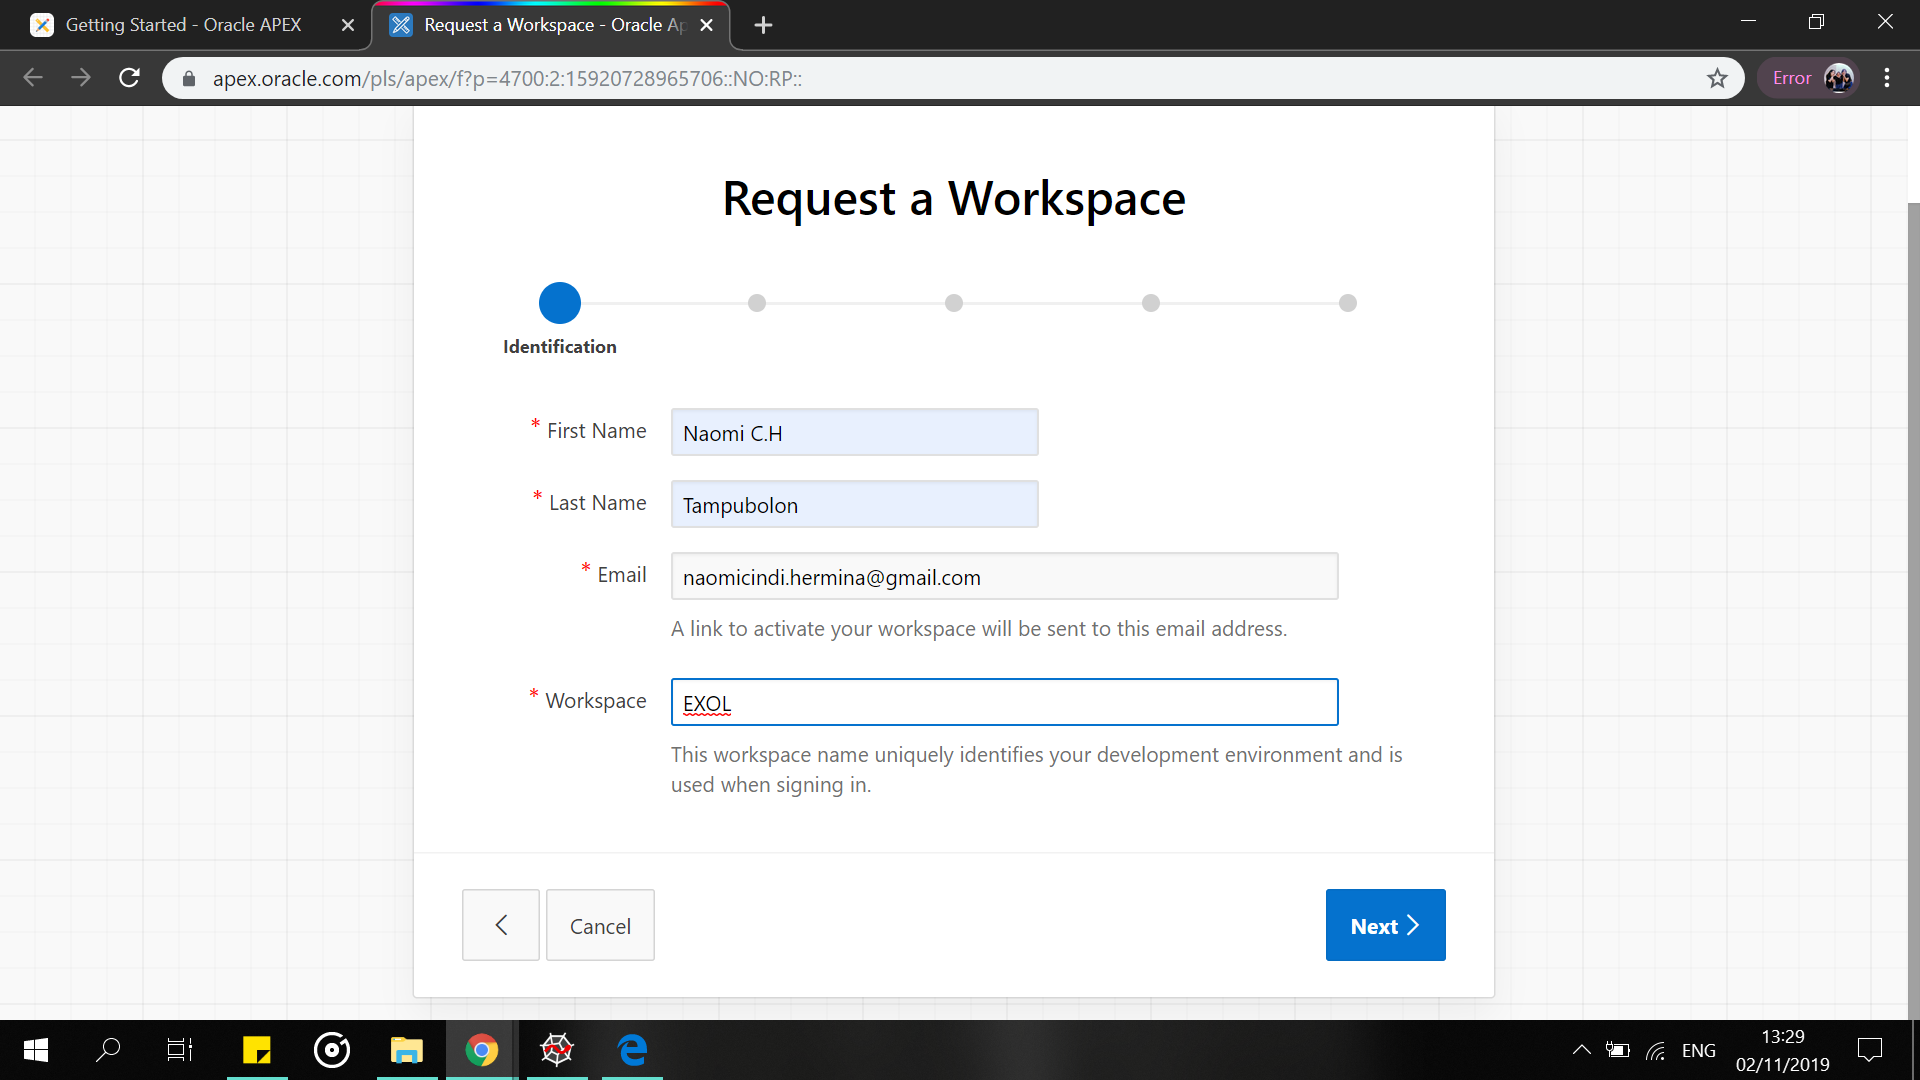
\includegraphics[width=9cm]{picture/06.png}
    \caption{Contoh Mengisi Form}
    \end{figure}
    
\item Ikuti langkah berikut. kemudian pilih "yes".
    \begin{figure}[!htbp]
    \centering
    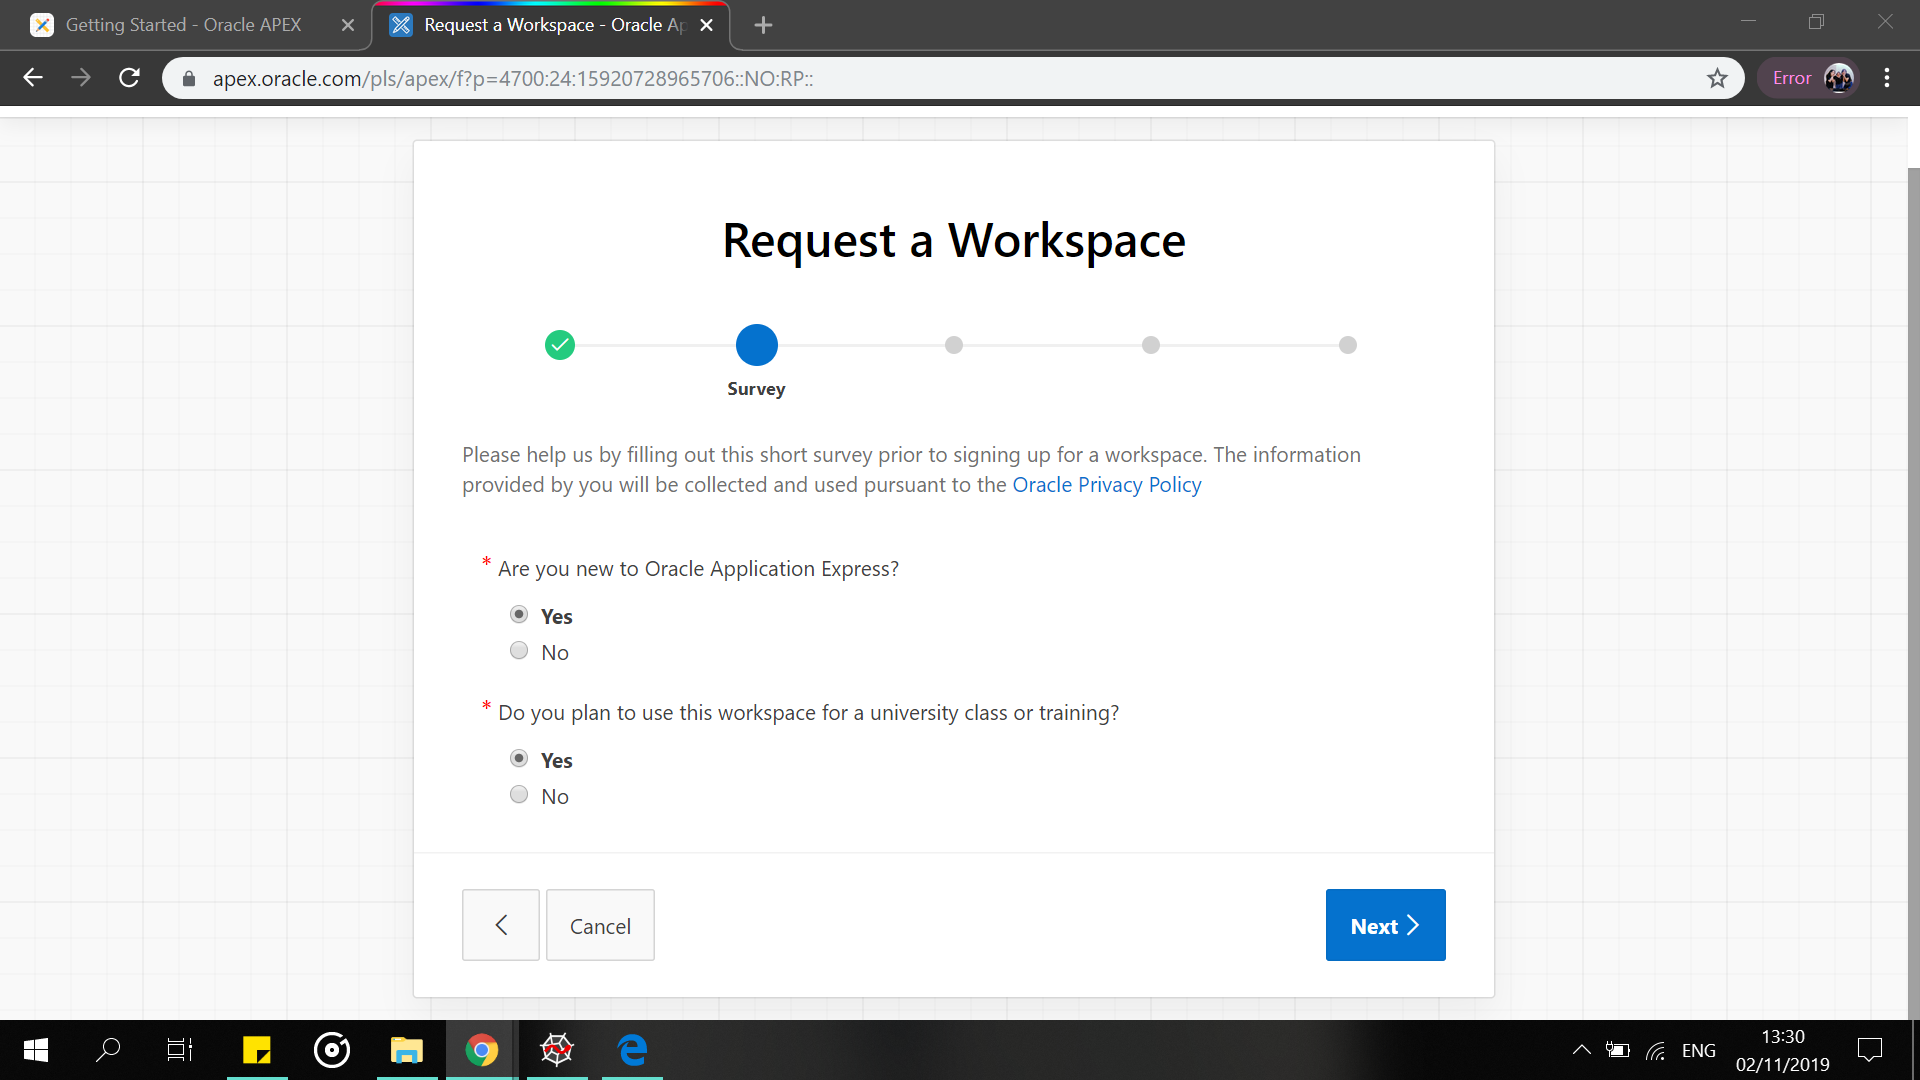
\includegraphics[width=9cm]{picture/07.png}
    \caption{Contoh Mengisi Form}
    \end{figure}
    
\item Kemudian isi alasan kita membuat sebuah Permintaan Workspace.
    \begin{figure}[!htbp]
    \centering
    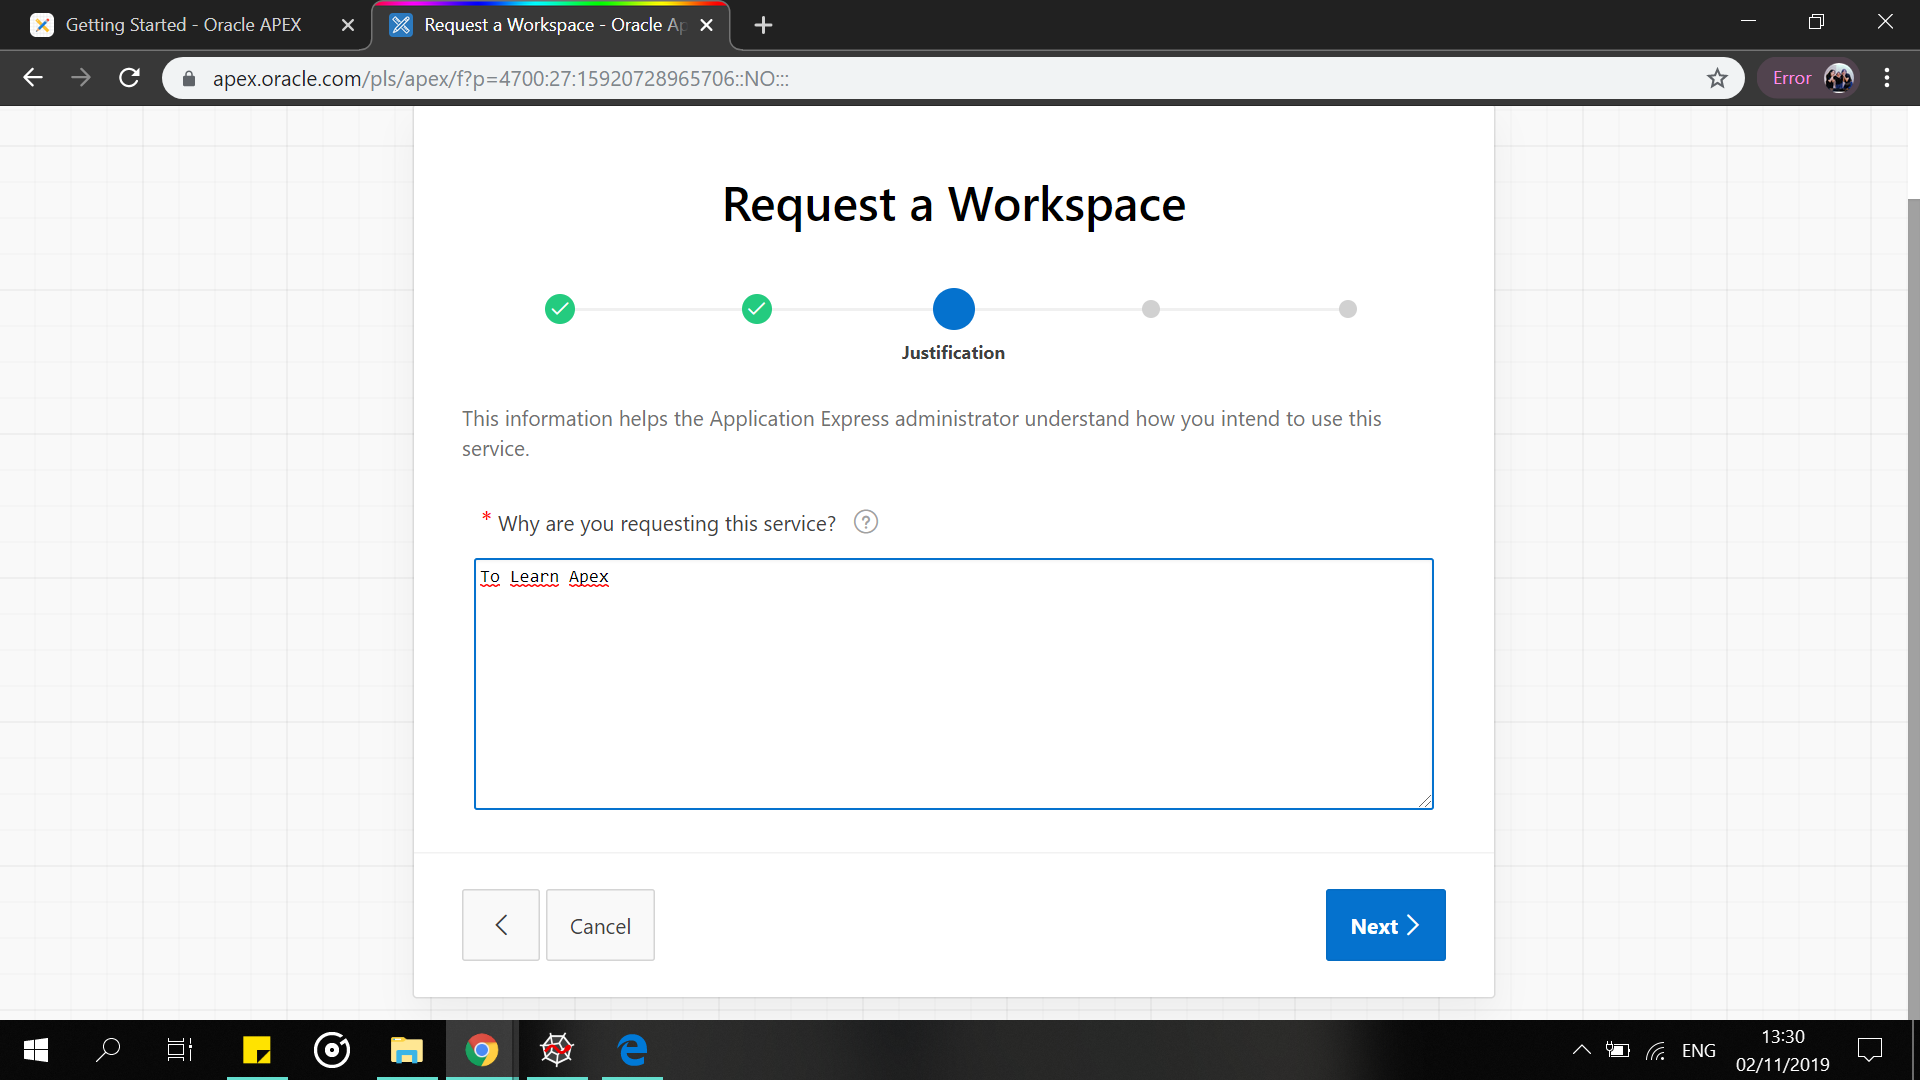
\includegraphics[width=9cm]{picture/08.png}
    \caption{Contoh Mengisi Form}
    \end{figure}
    
\newpage
\item Kemudian centang "I accept the terms".
    \begin{figure}[!htbp]
    \centering
    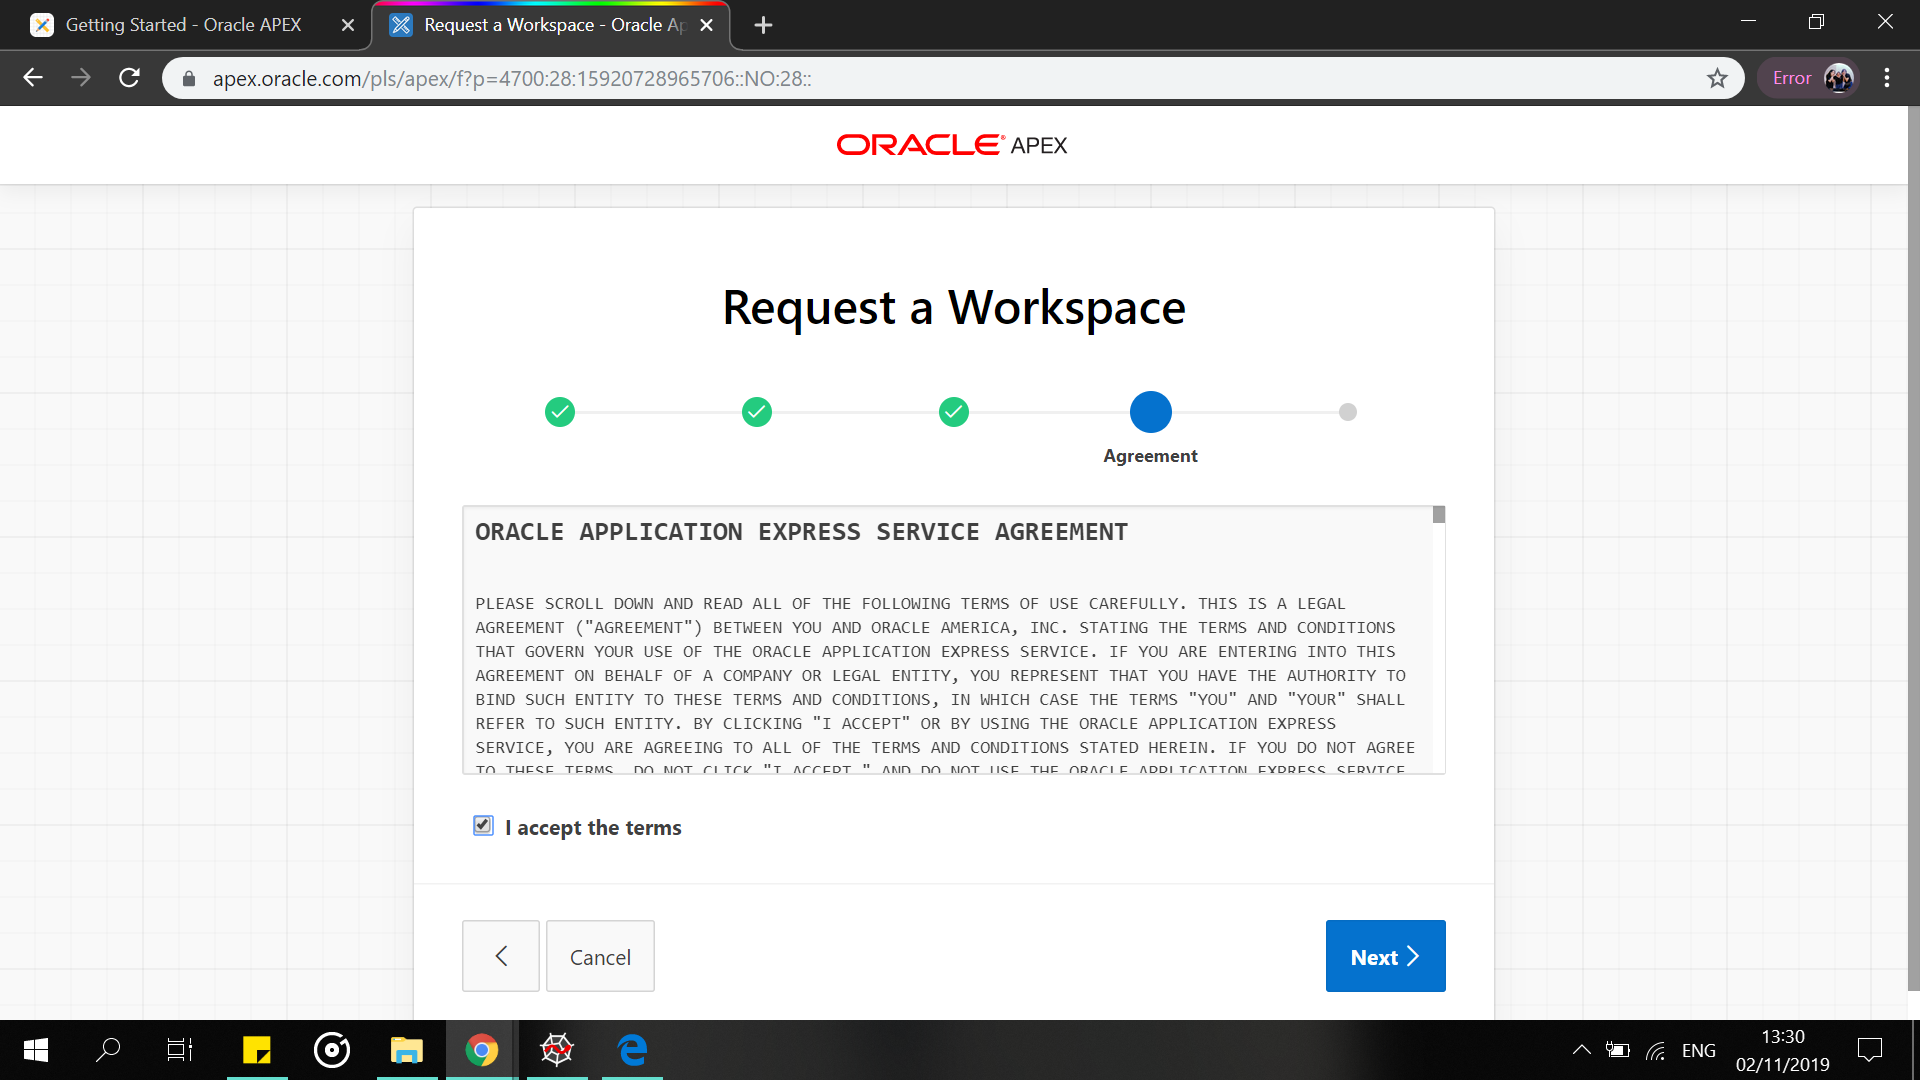
\includegraphics[width=9cm]{picture/09.png}
    \caption{Contoh Mengisi Form}
    \end{figure}
    
\item Kemudian klik "Submit Request".
    \begin{figure}[!htbp]
    \centering
    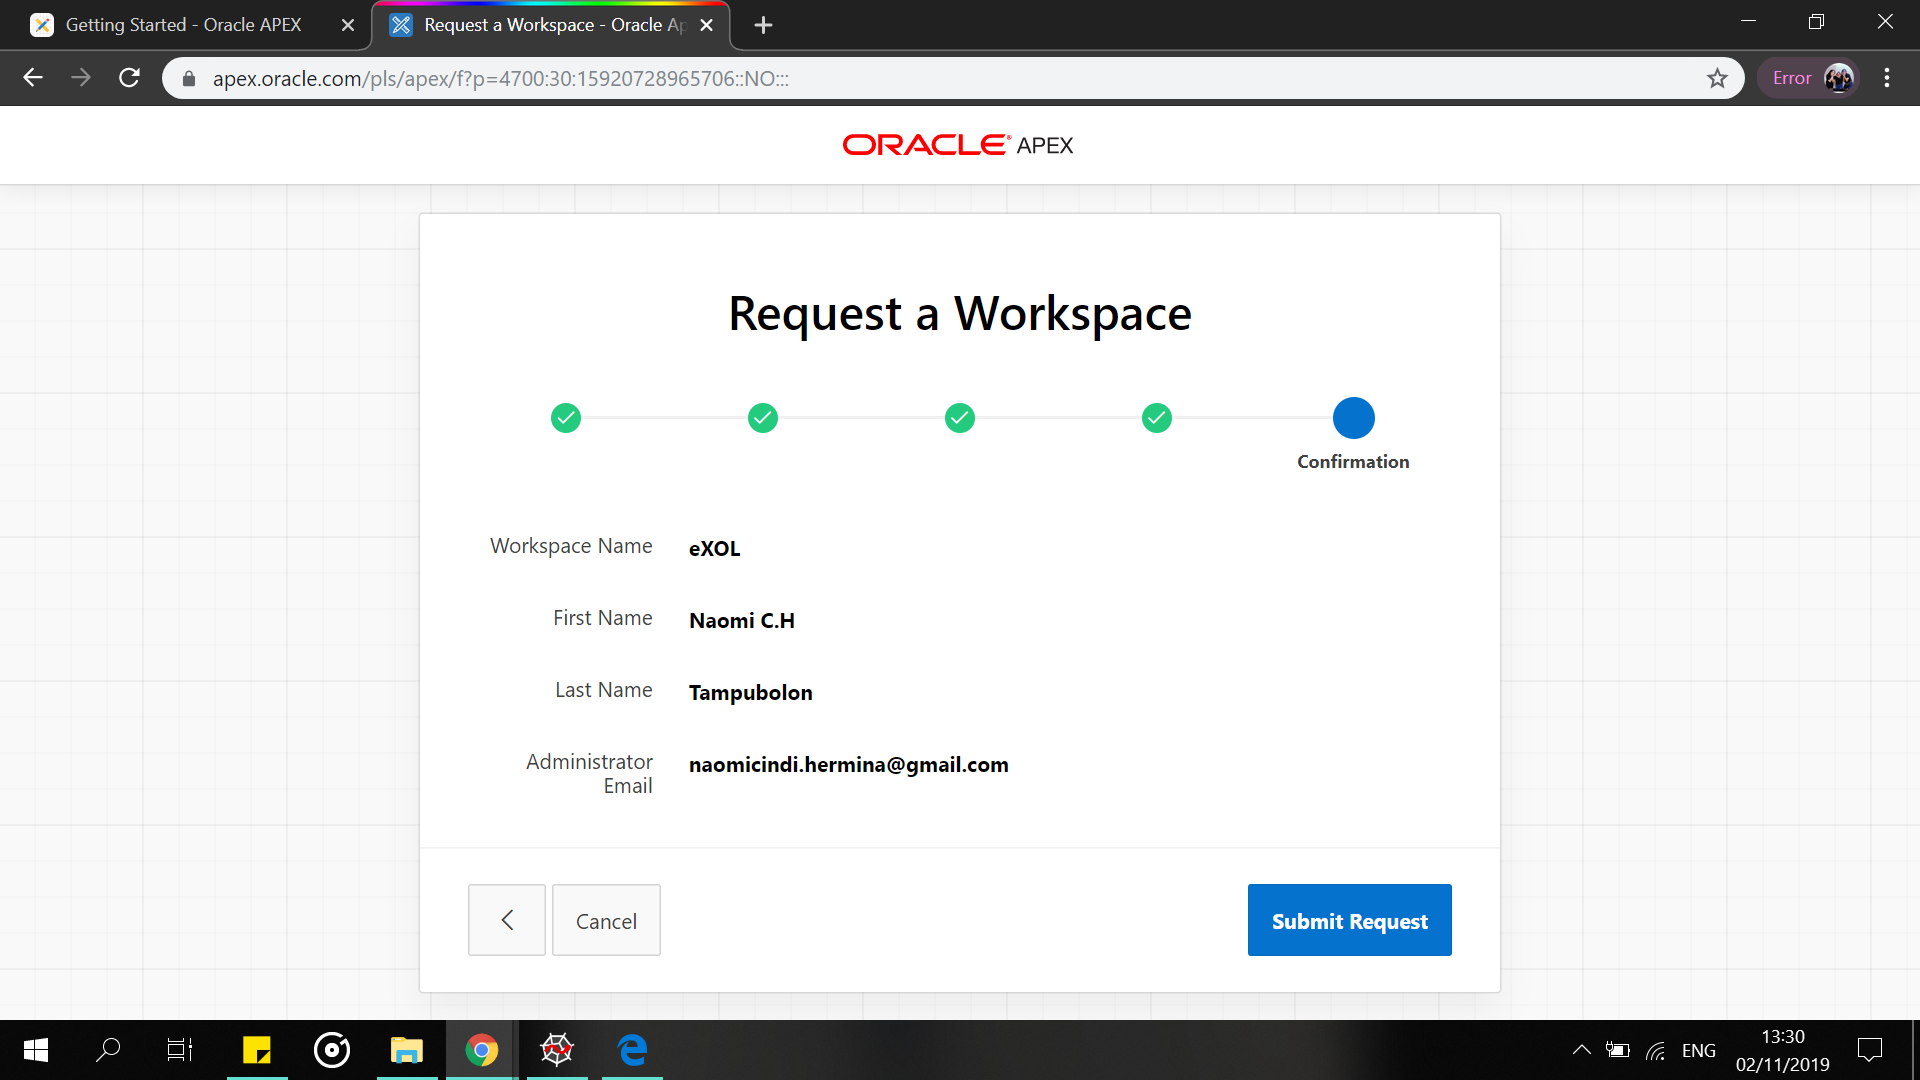
\includegraphics[width=9cm]{picture/10.png}
    \caption{Contoh Form Telah Terisi}
    \end{figure}
    
\item Permintaan Workspace baru telah berhasil.
    \begin{figure}[!htbp]
    \centering
    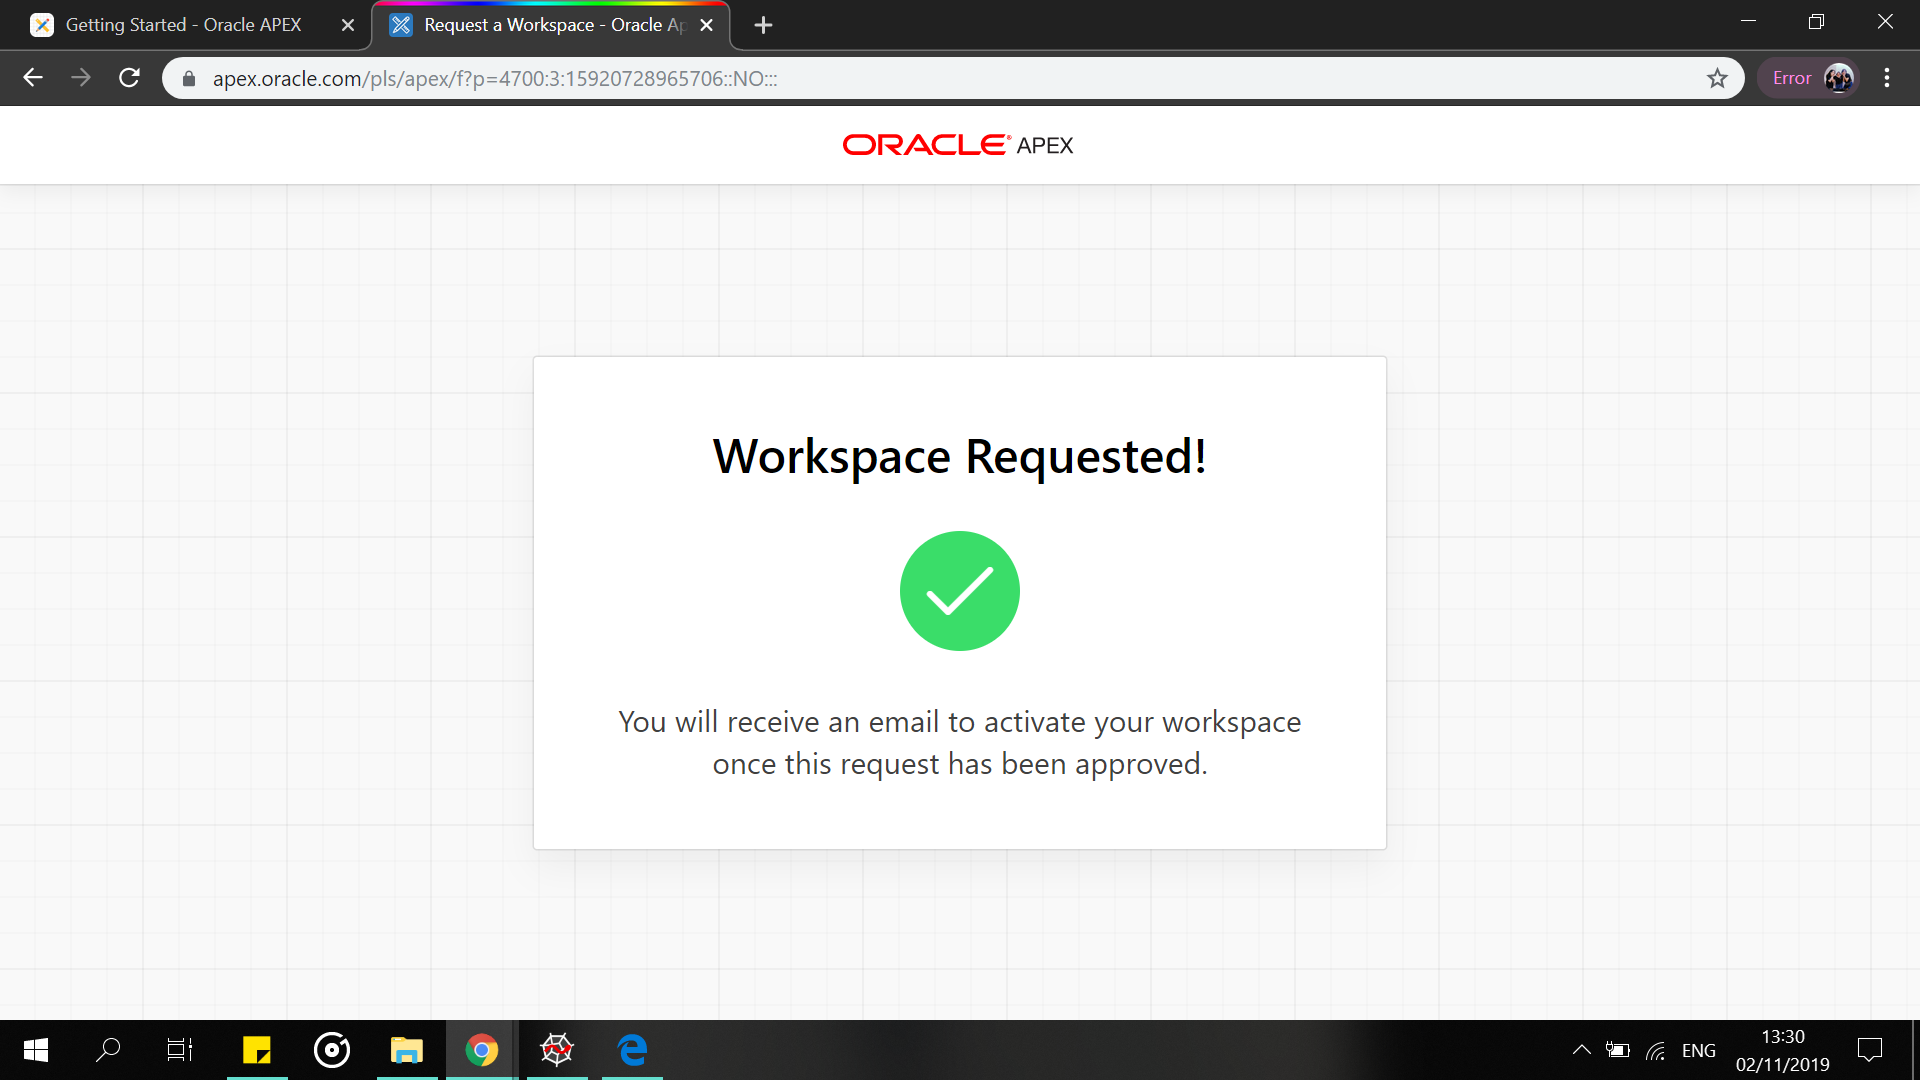
\includegraphics[width=9cm]{picture/11.png}
    \caption{Contoh Permintaan Workspace Baru}
    \end{figure}
        
\newpage
\item Buka email yang telah di daftarkan pada oracle apex.
    \begin{figure}[!htbp]
    \centering
    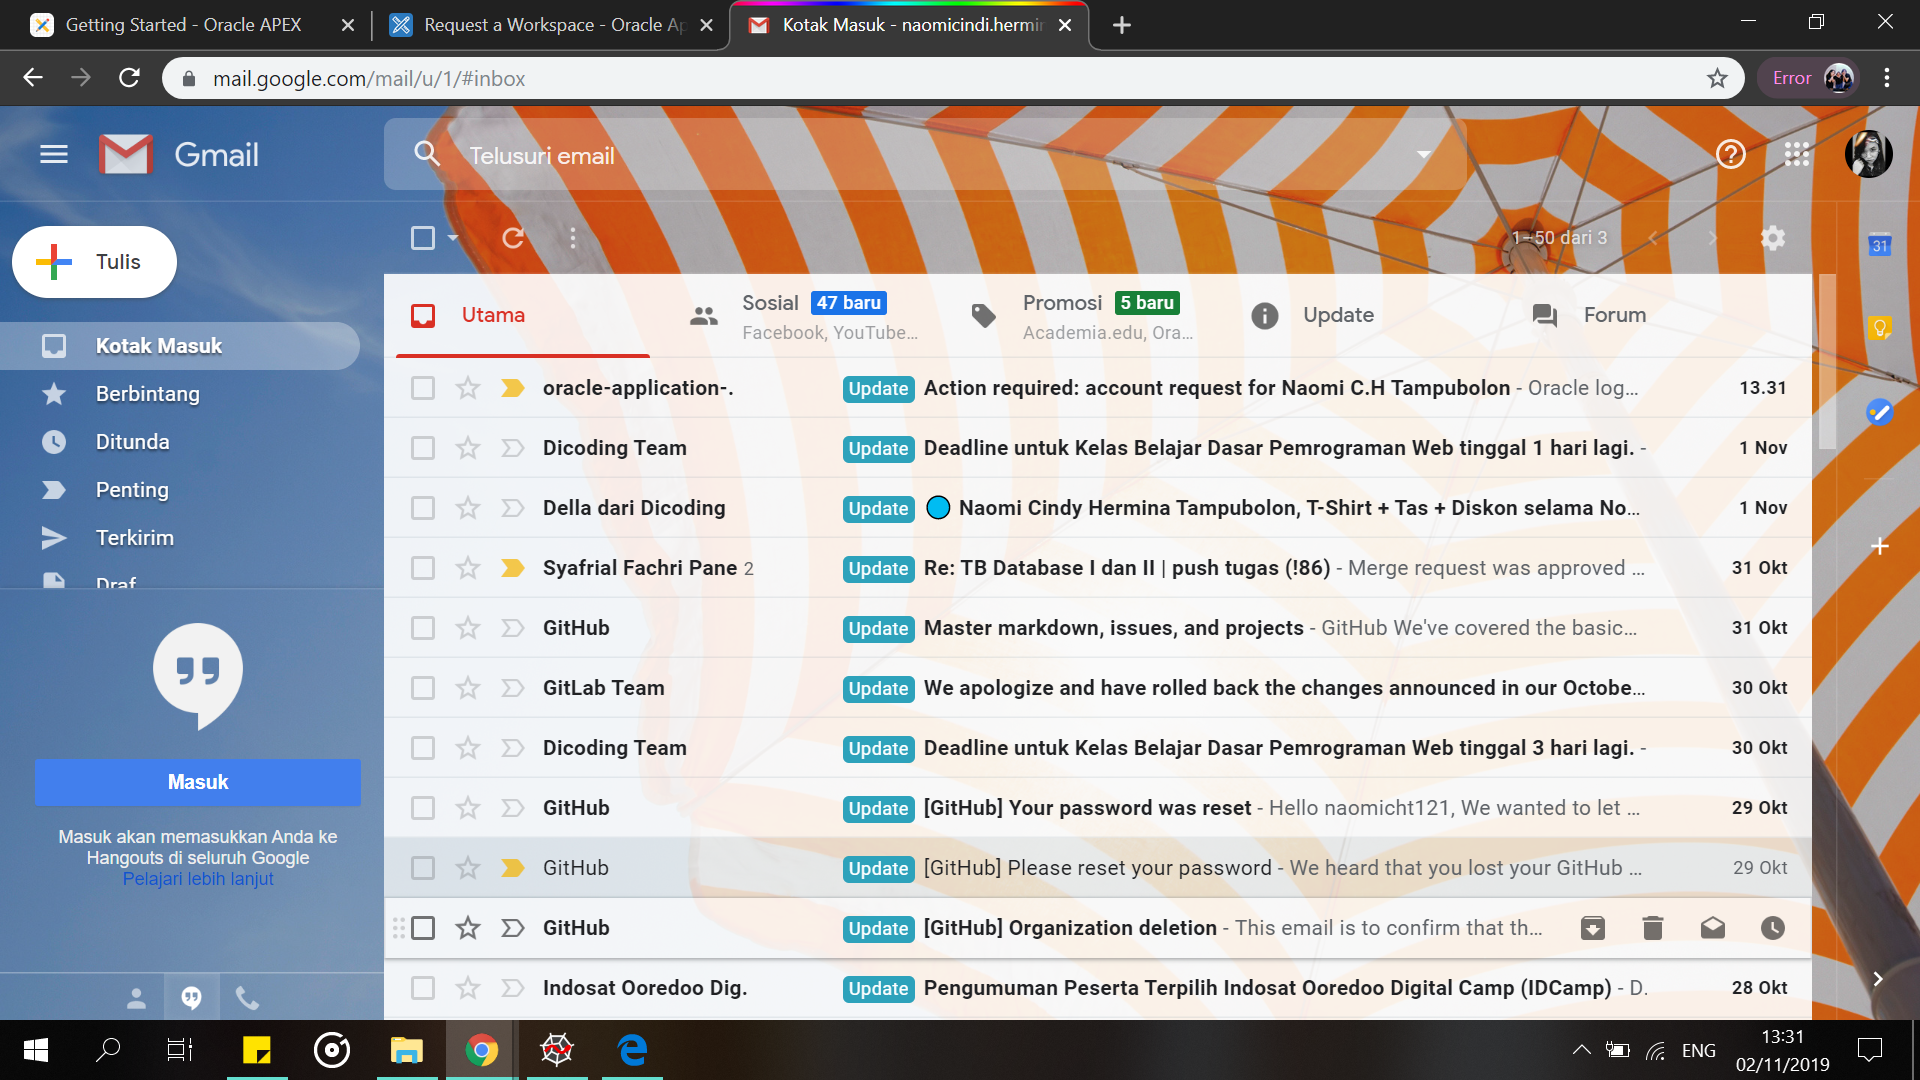
\includegraphics[width=9cm]{picture/12.png}
    \caption{Contoh Verifikasi Email}
    \end{figure}
    
\item Buka Pesan dari Oracle Apex.
    \begin{figure}[!htbp]
    \centering
    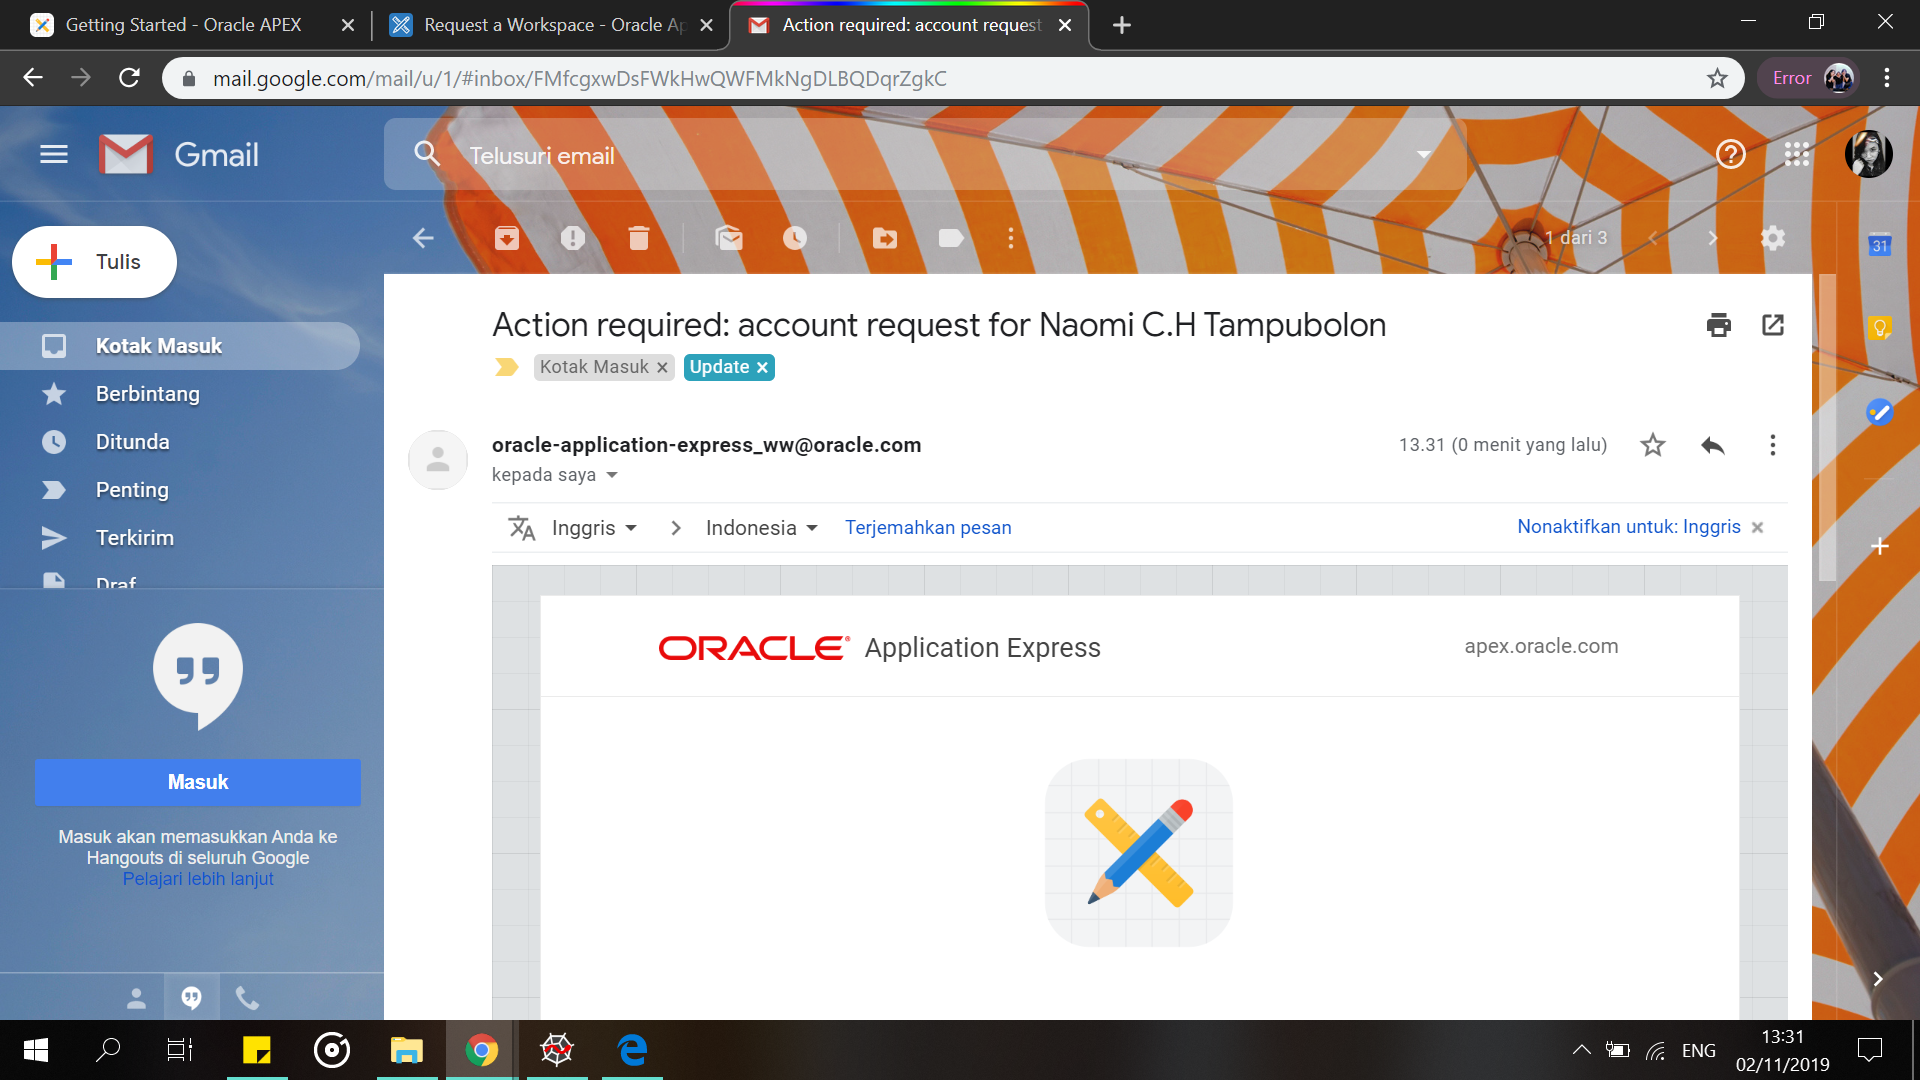
\includegraphics[width=9cm]{picture/13.png}
    \caption{Contoh Verifikasi Email}
    \end{figure}
    
\item Kemudian klik "Create Workspace" untuk membuat workspace yang baru.
    \begin{figure}[!htbp]
    \centering
    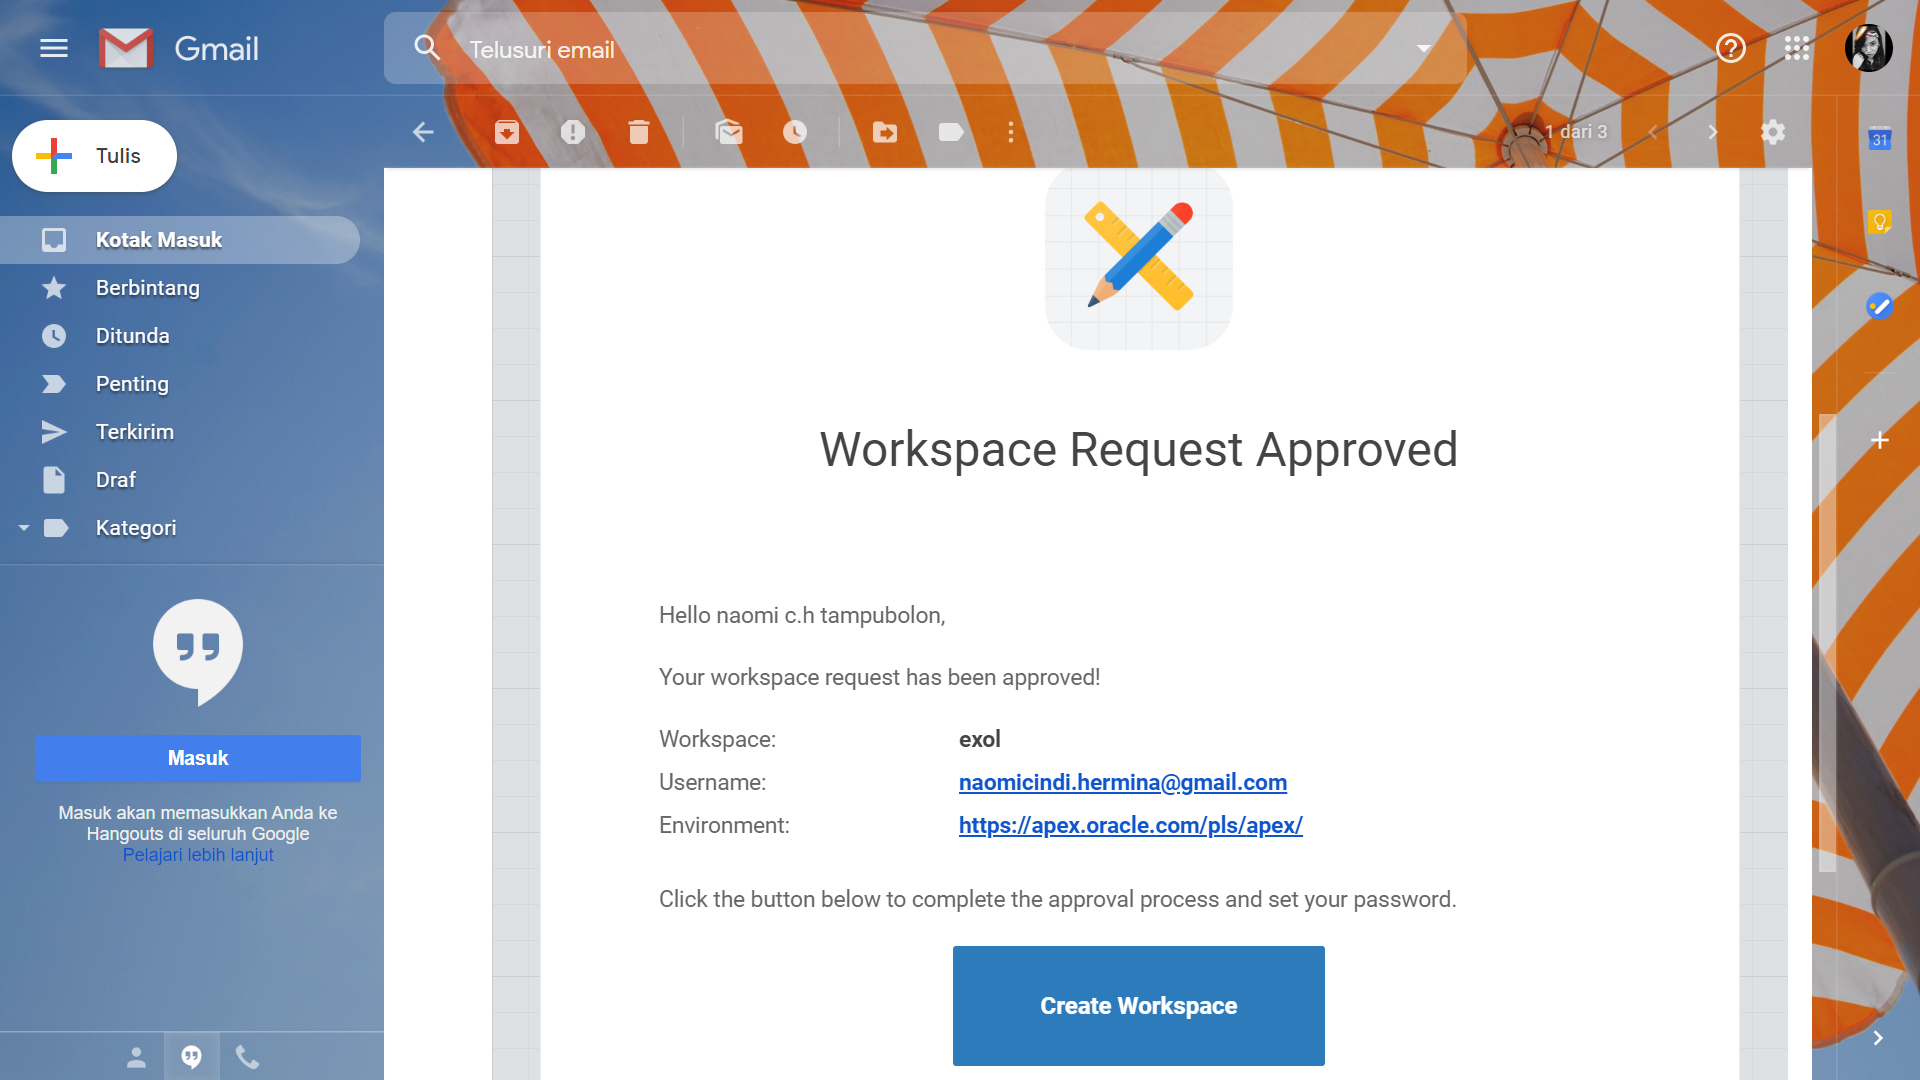
\includegraphics[width=9cm]{picture/14.png}
    \caption{Contoh Verifikasi Email}
    \end{figure}
    
\newpage
\item Akan muncul gambar sebagai berikut, lalu klik "Continue to Sign In Screen"
    \begin{figure}[!htbp]
    \centering
    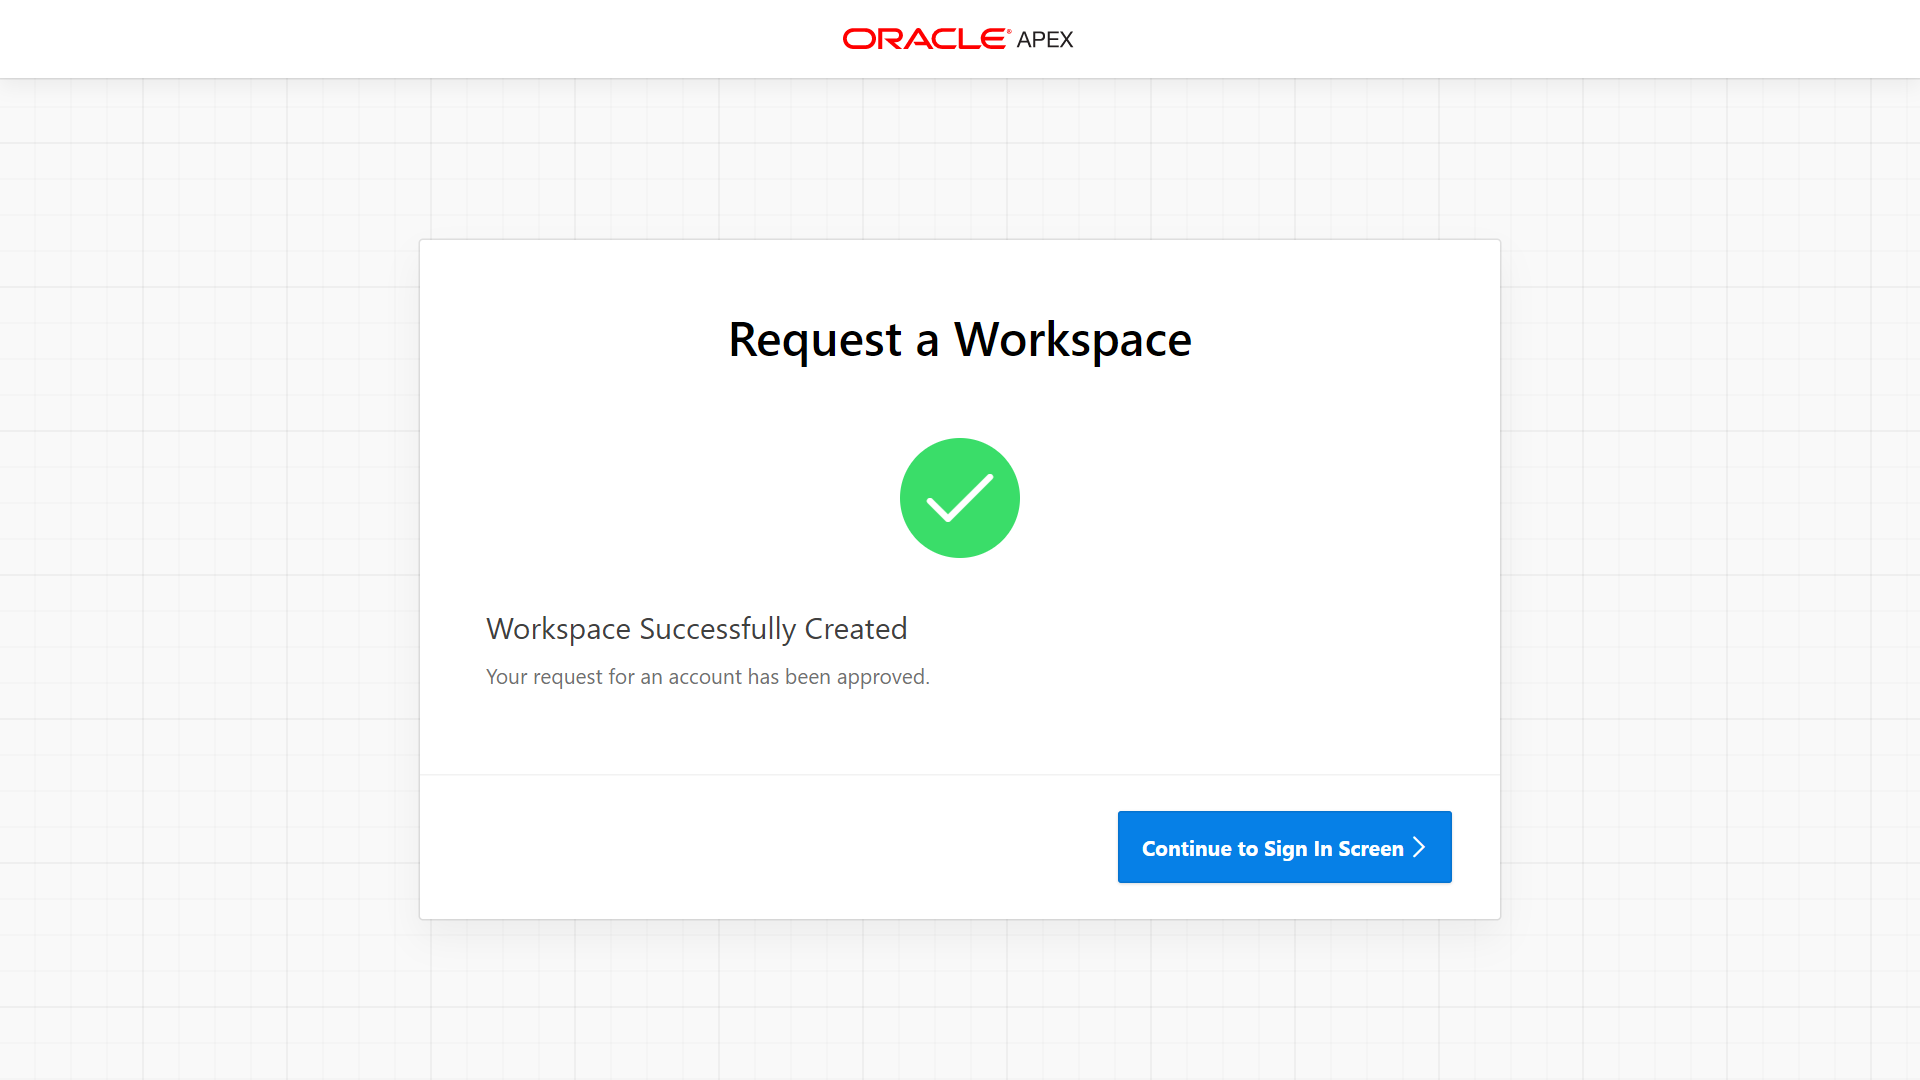
\includegraphics[width=8cm]{picture/15.png}
    \caption{Contoh Workspace telah terbentuk}
    \end{figure}
    
\item Kemudian isi email dan masukkan password.
    \begin{figure}[!htbp]
    \centering
    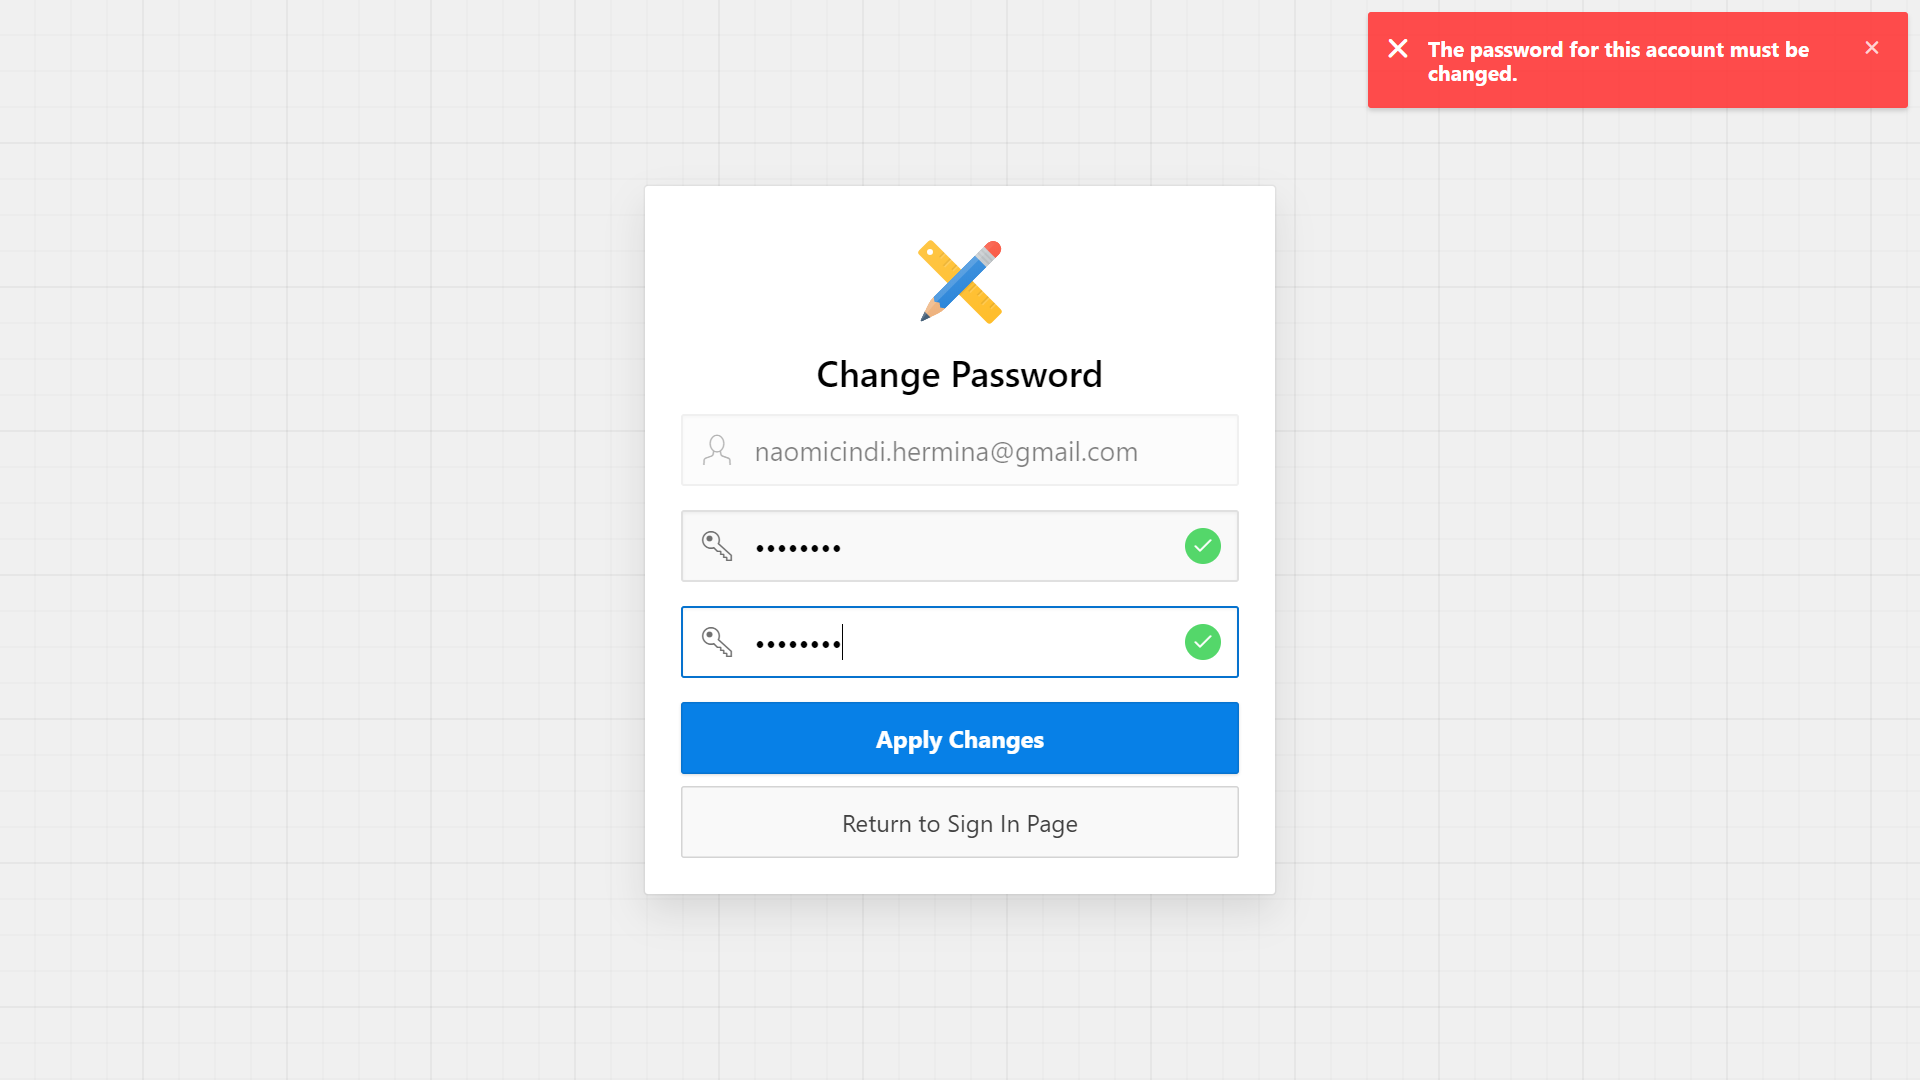
\includegraphics[width=8cm]{picture/16.png}
    \caption{Contoh Memasukkan Password}
    \end{figure}
    
\item Tampilan Workspace Oracle Apex. Langkah selanjutnya klik "App Builder" seperti gambar berikut:
    \begin{figure}[!htbp]
    \centering
    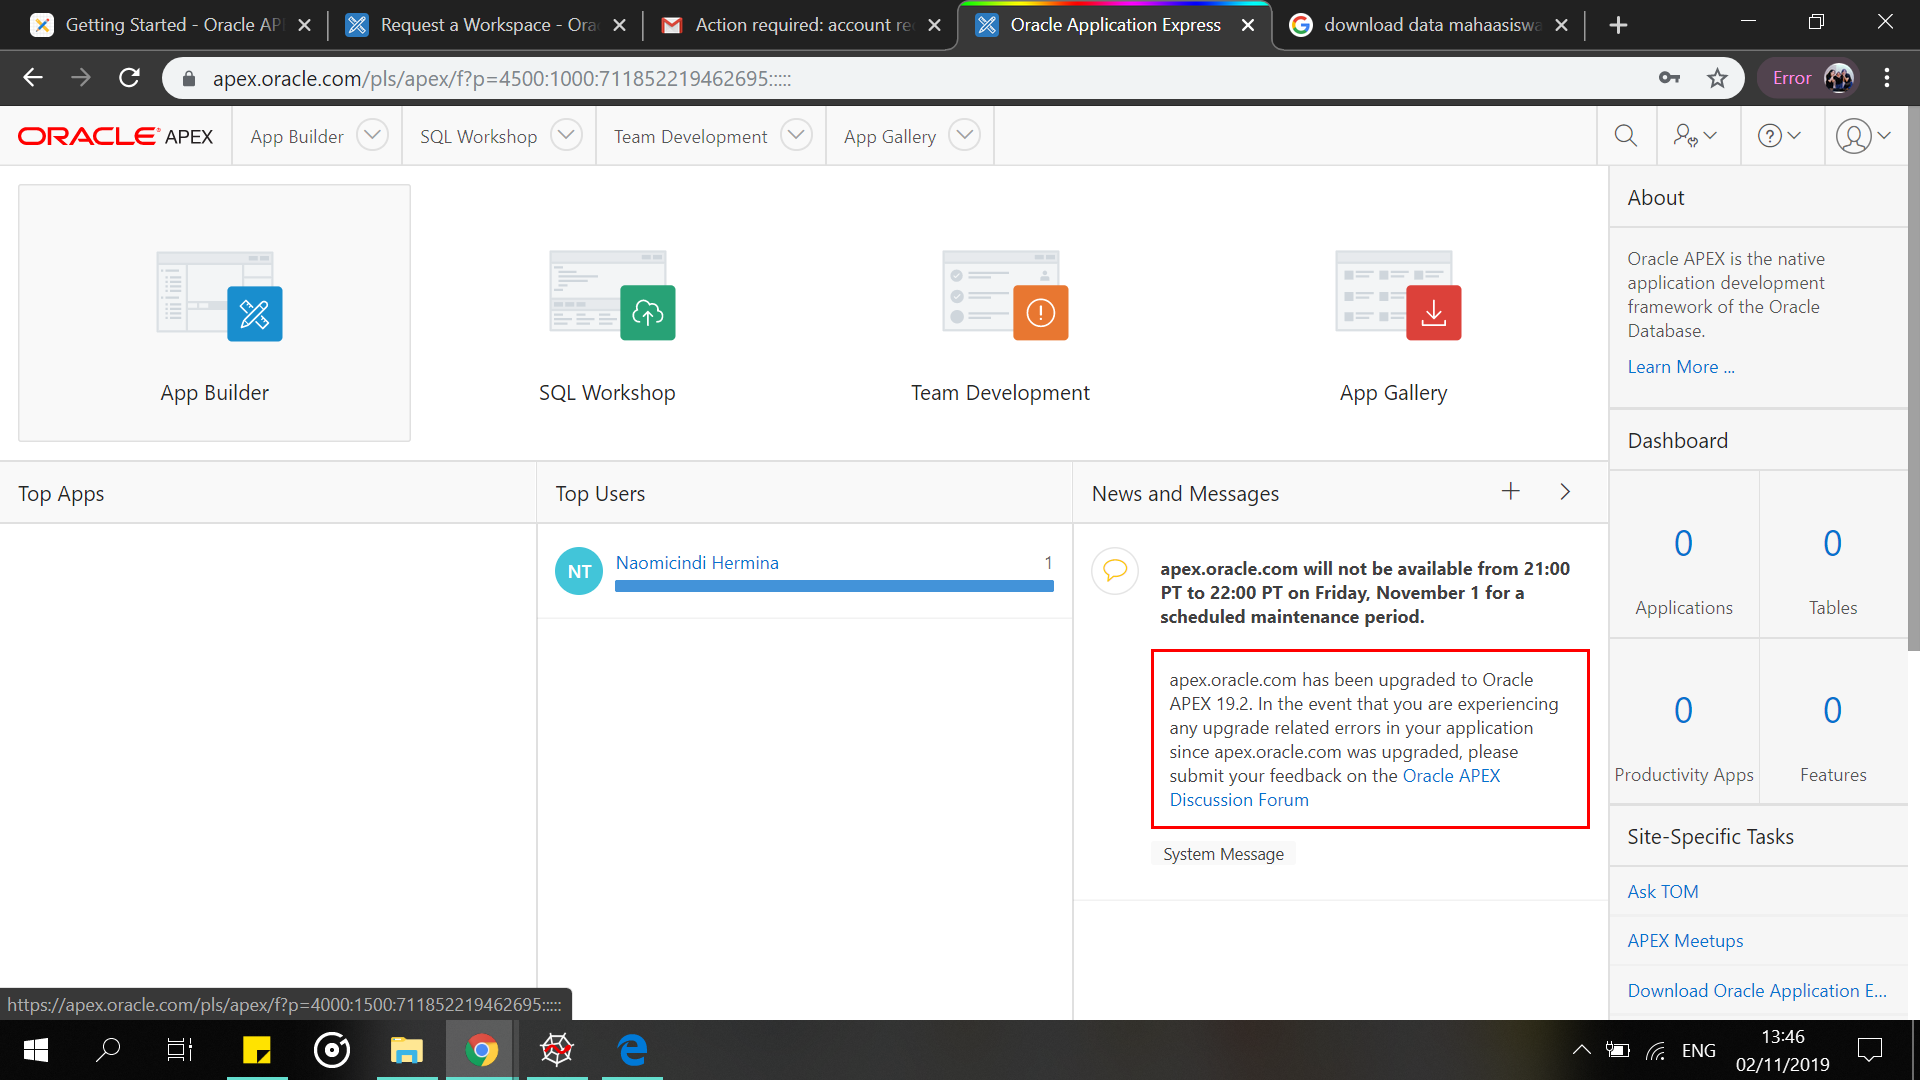
\includegraphics[width=8cm]{picture/17.png}
    \caption{Contoh Verifikasi Email}
    \end{figure}
    
\newpage
\item Kemudian klik "Create a new App" untuk membuat aplikasi di Application Express.
    \begin{figure}[!htbp]
    \centering
    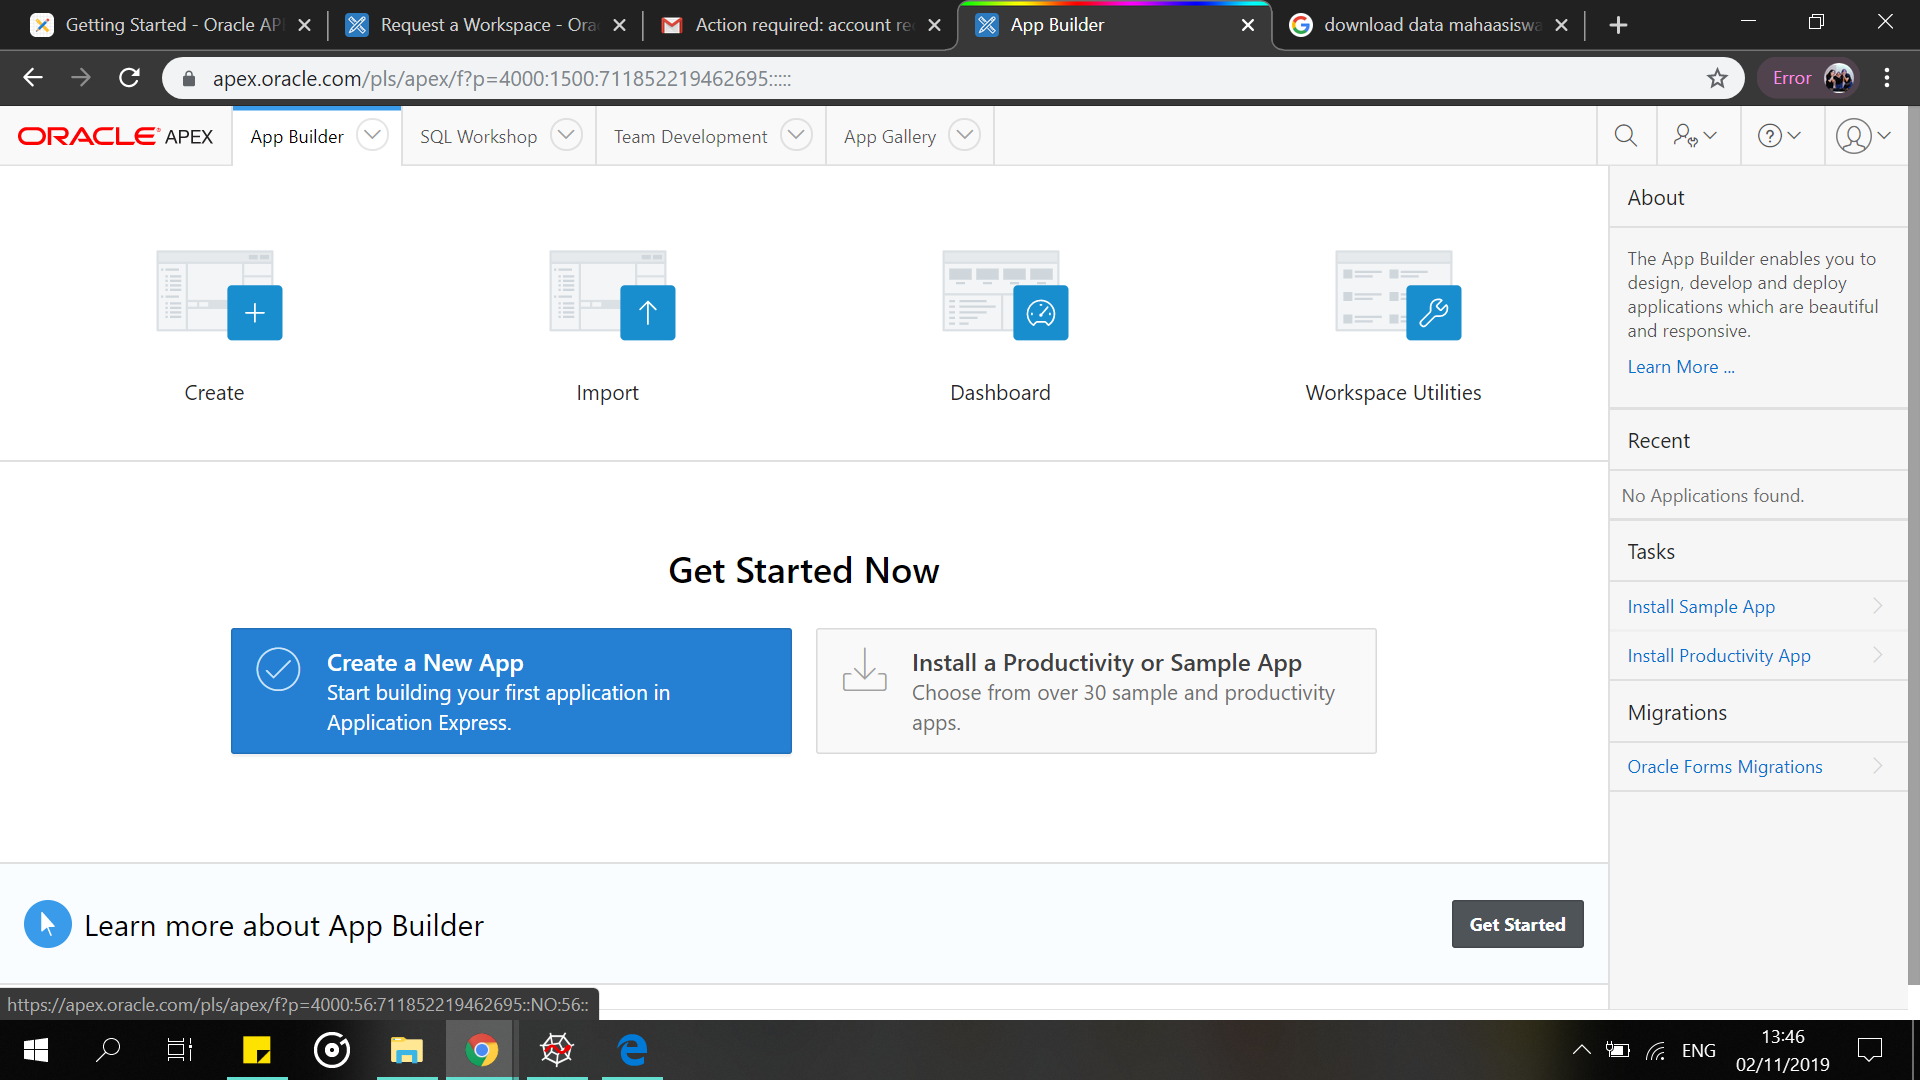
\includegraphics[width=8cm]{picture/18.png}
    \caption{Contoh Membuat Aplikasi}
    \end{figure}
    
\item Kemudian klik "From a File" untuk mengupload file.
    \begin{figure}[!htbp]
    \centering
    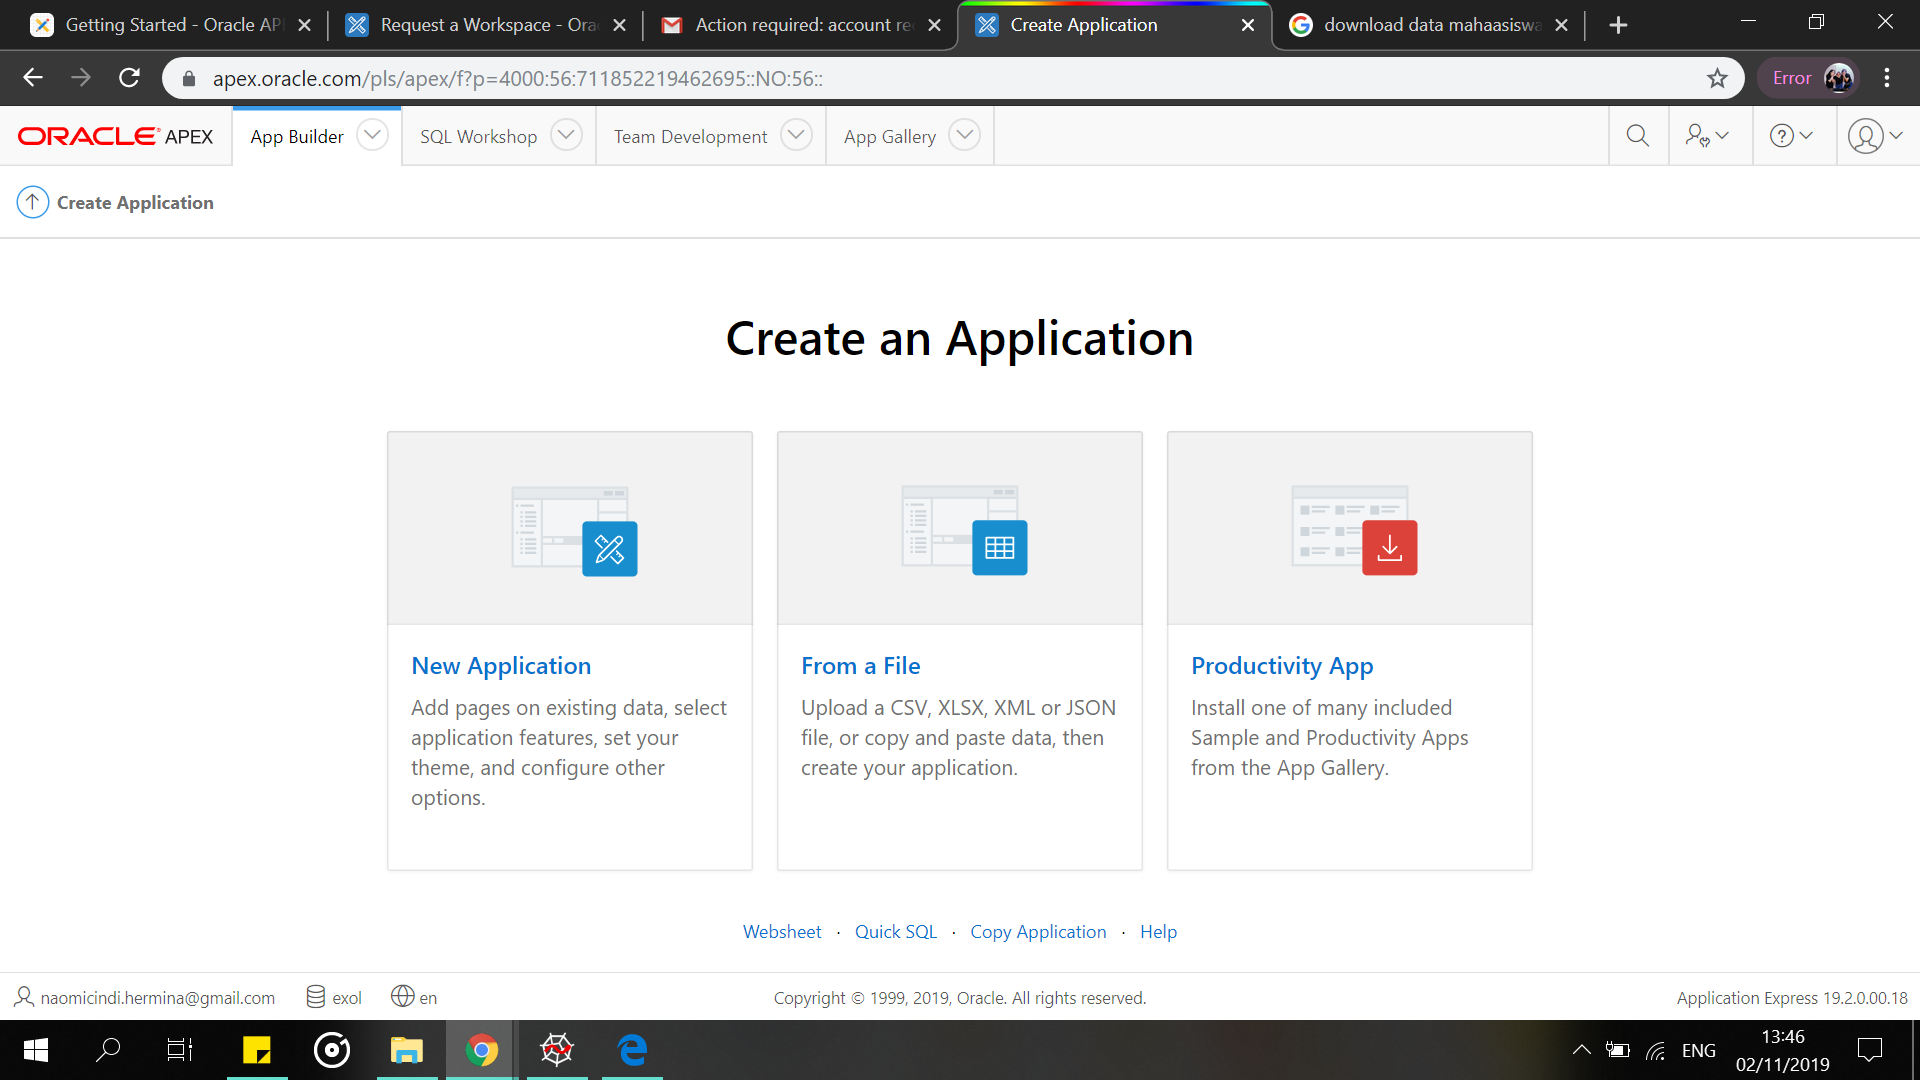
\includegraphics[width=8cm]{picture/19.png}
    \caption{Contoh Upoad file}
    \end{figure}
    
\item Kemudian klik "Drag and Drop file" untuk mengupload file data yang sudah ada.
    \begin{figure}[!htbp]
    \centering
    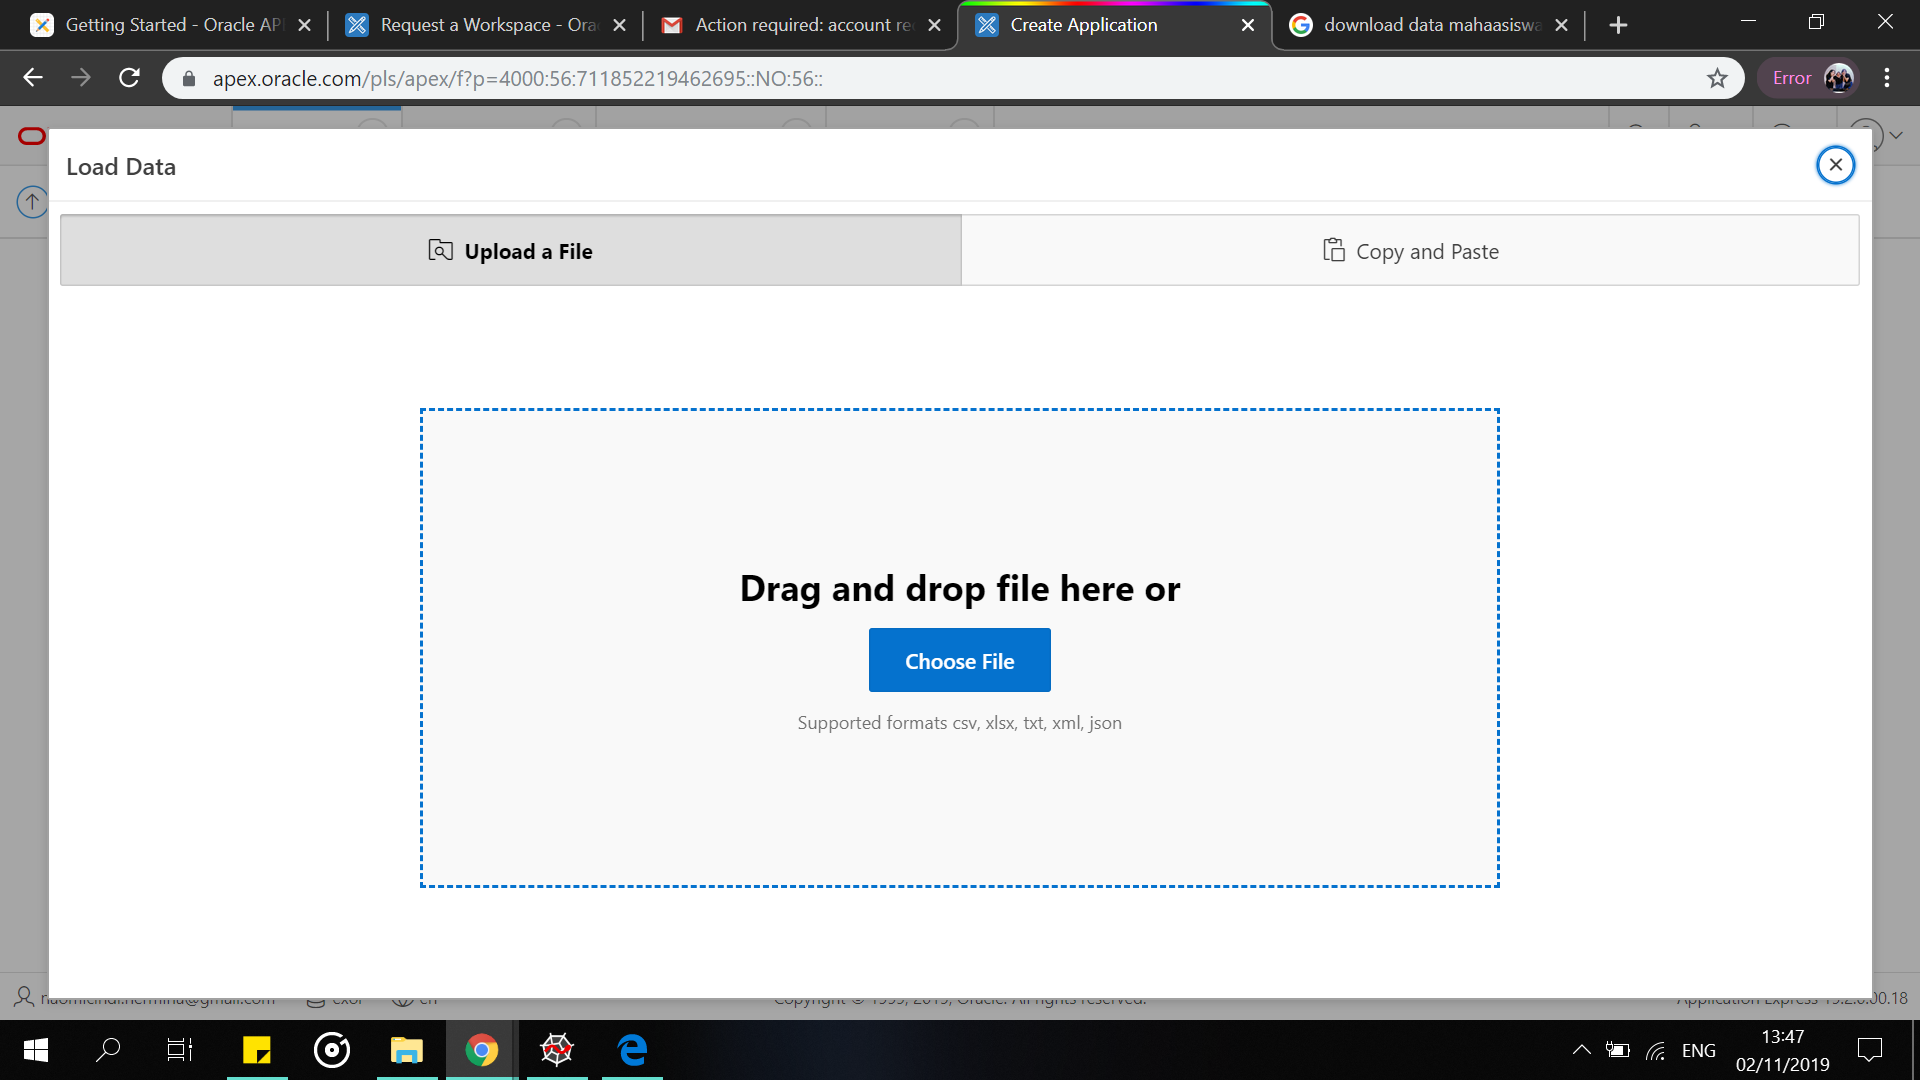
\includegraphics[width=8cm]{picture/20.png}
    \caption{Contoh Upload File}
    \end{figure}
    
\newpage
\item Pilih data yang akan di Upload. Contoh data yang sudah kita buat sebelumnya.
    \begin{figure}[!htbp]
    \centering
    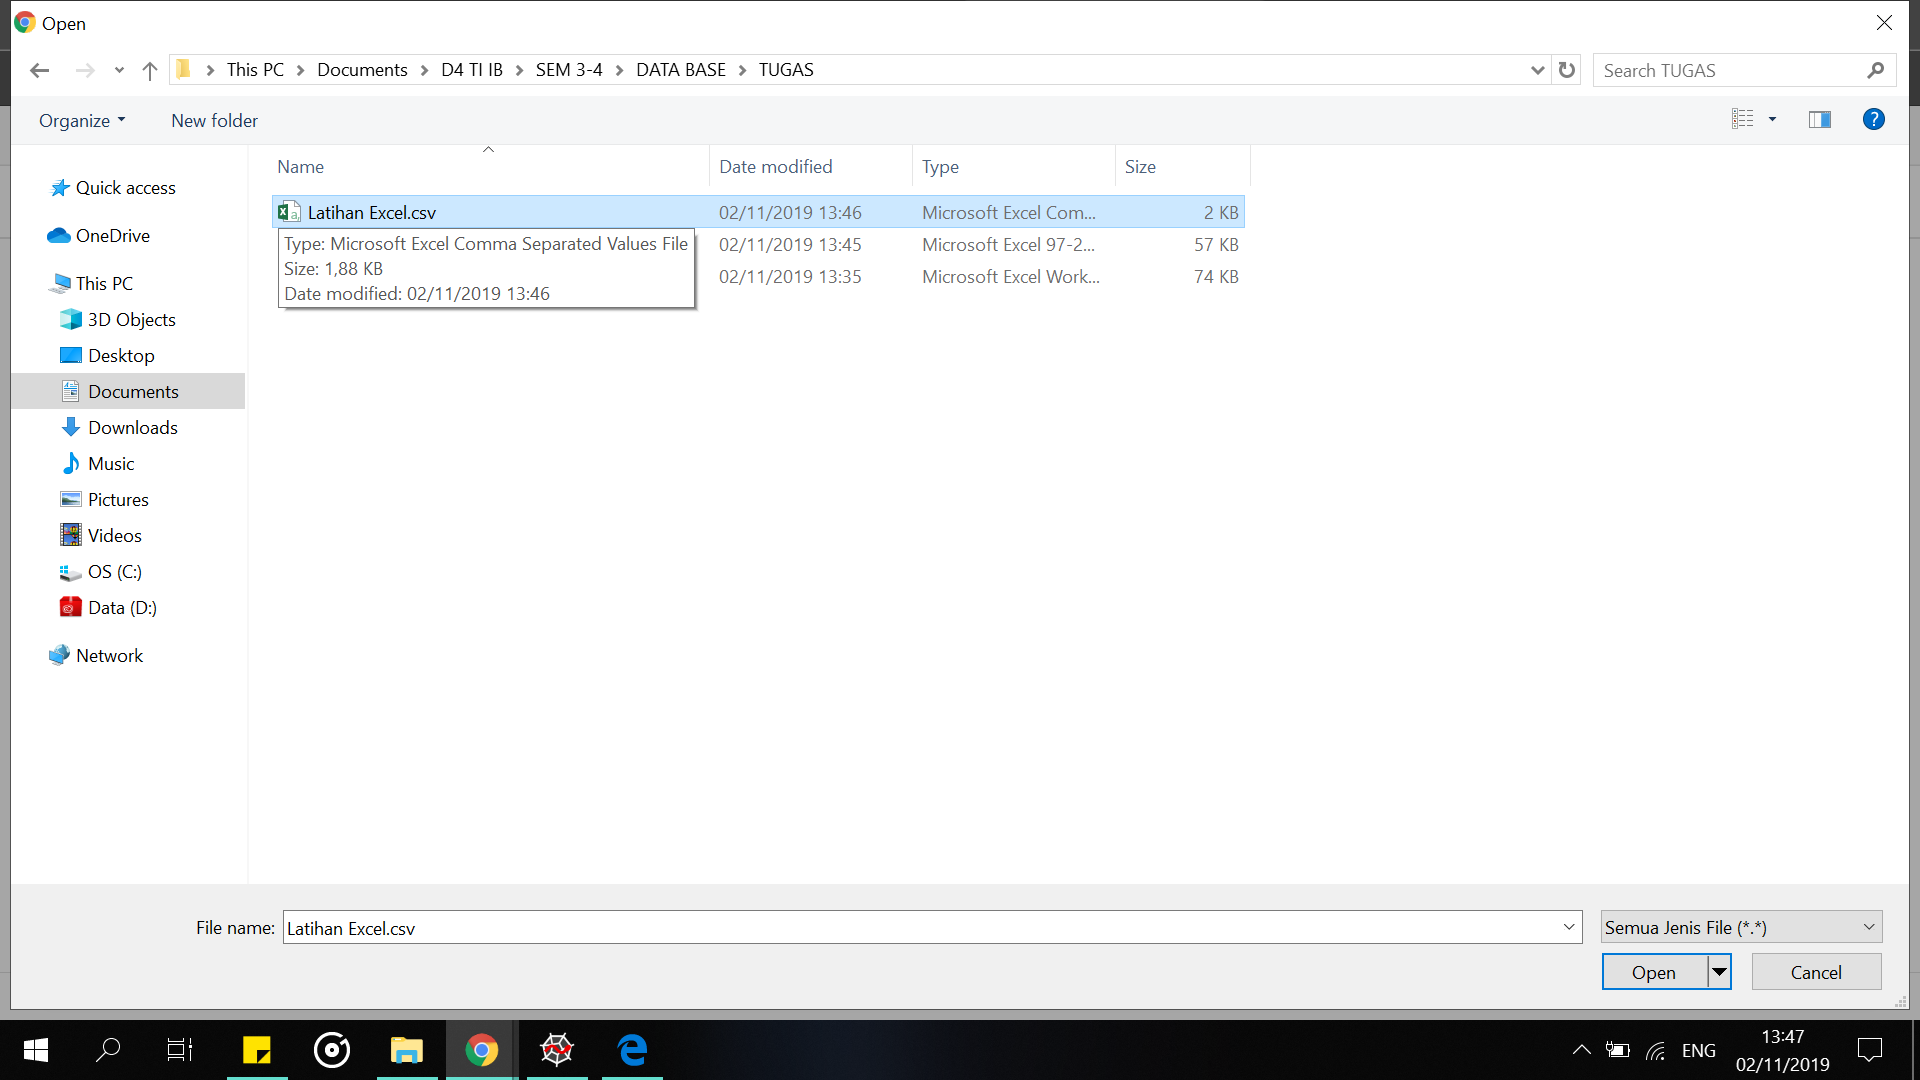
\includegraphics[width=8cm]{picture/21.png}
    \caption{Contoh Pilih data yang akan di Upload}
    \end{figure}
    
\item Isi nama tabel Owner seperti contoh berikut dan pada tabel Name hanya mengklik saja, nanti namanya akan otomatis tampil.
    \begin{figure}[!htbp]
    \centering
    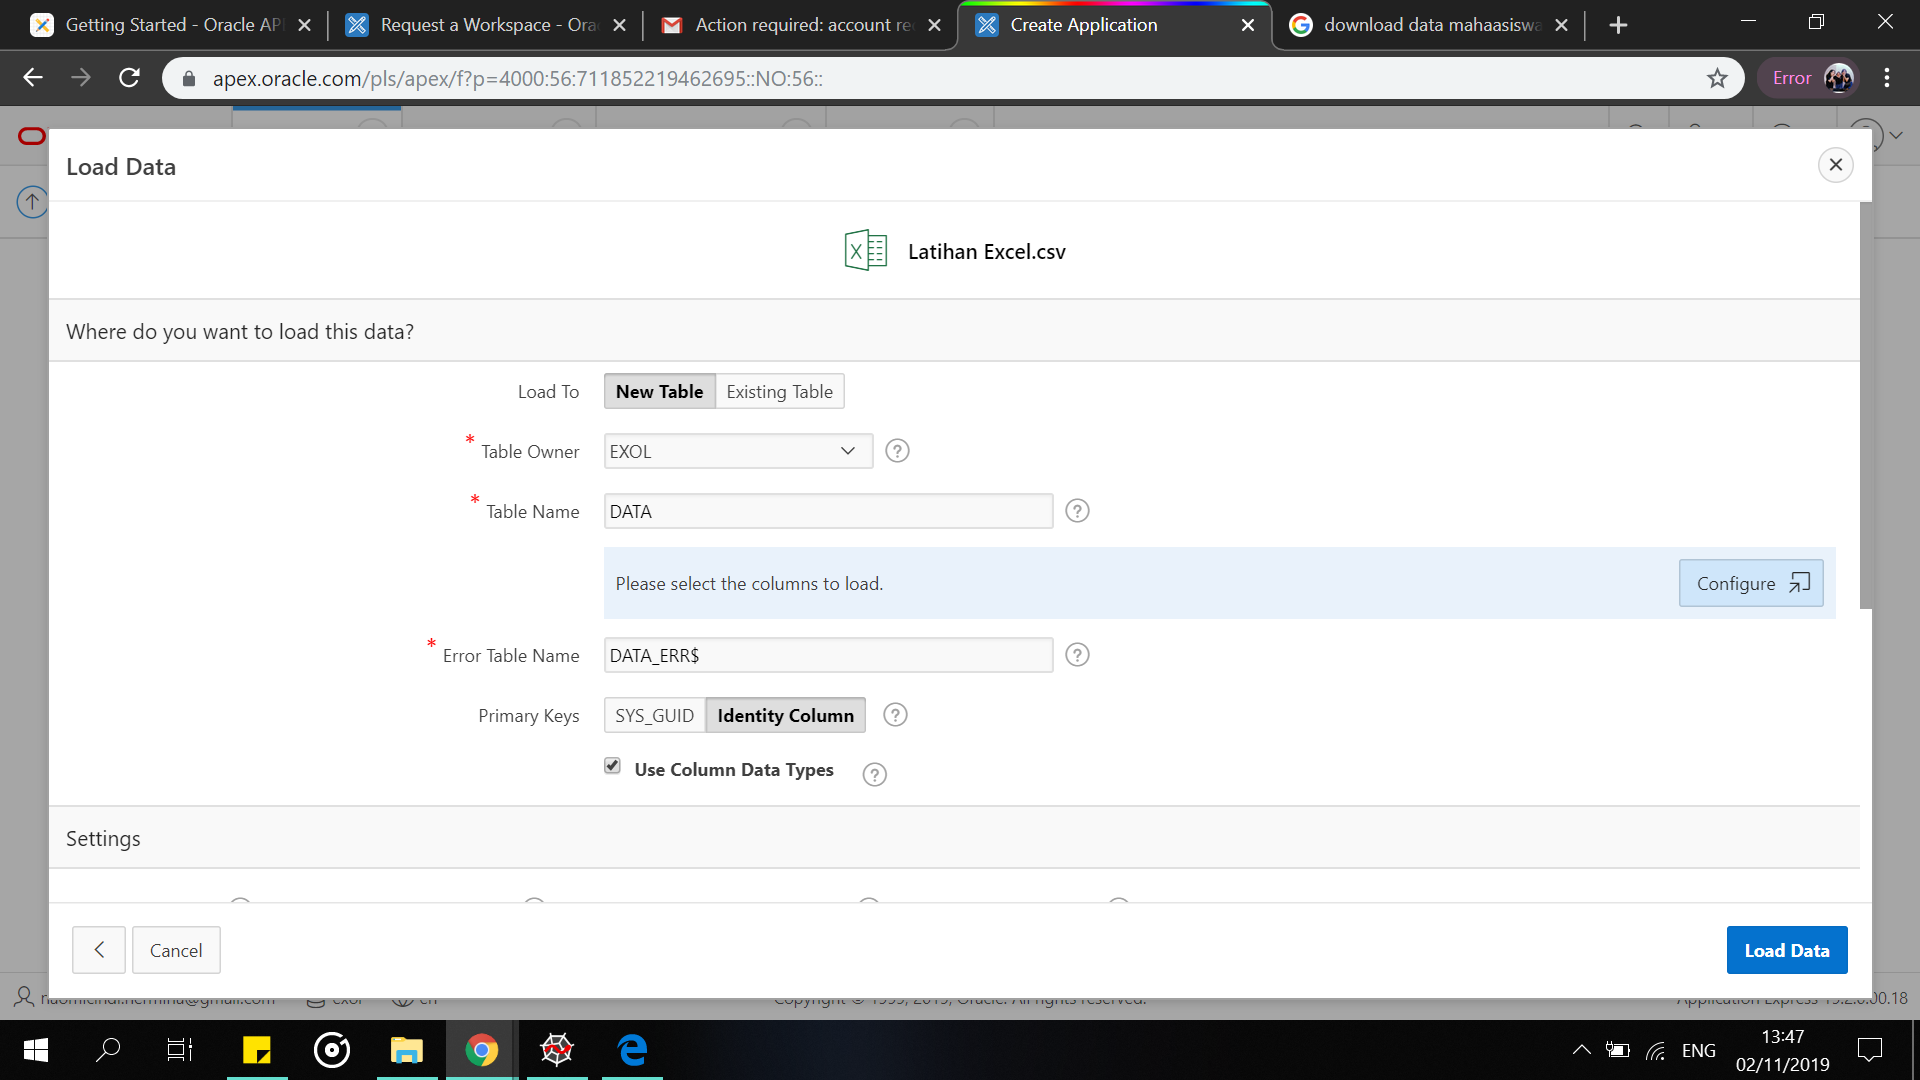
\includegraphics[width=8cm]{picture/22.png}
    \caption{Contoh Nama Tabel}
    \end{figure}

    
\item Ketik configure untuk tabel yang sudah di Upload..
    \begin{figure}[!htbp]
    \centering
    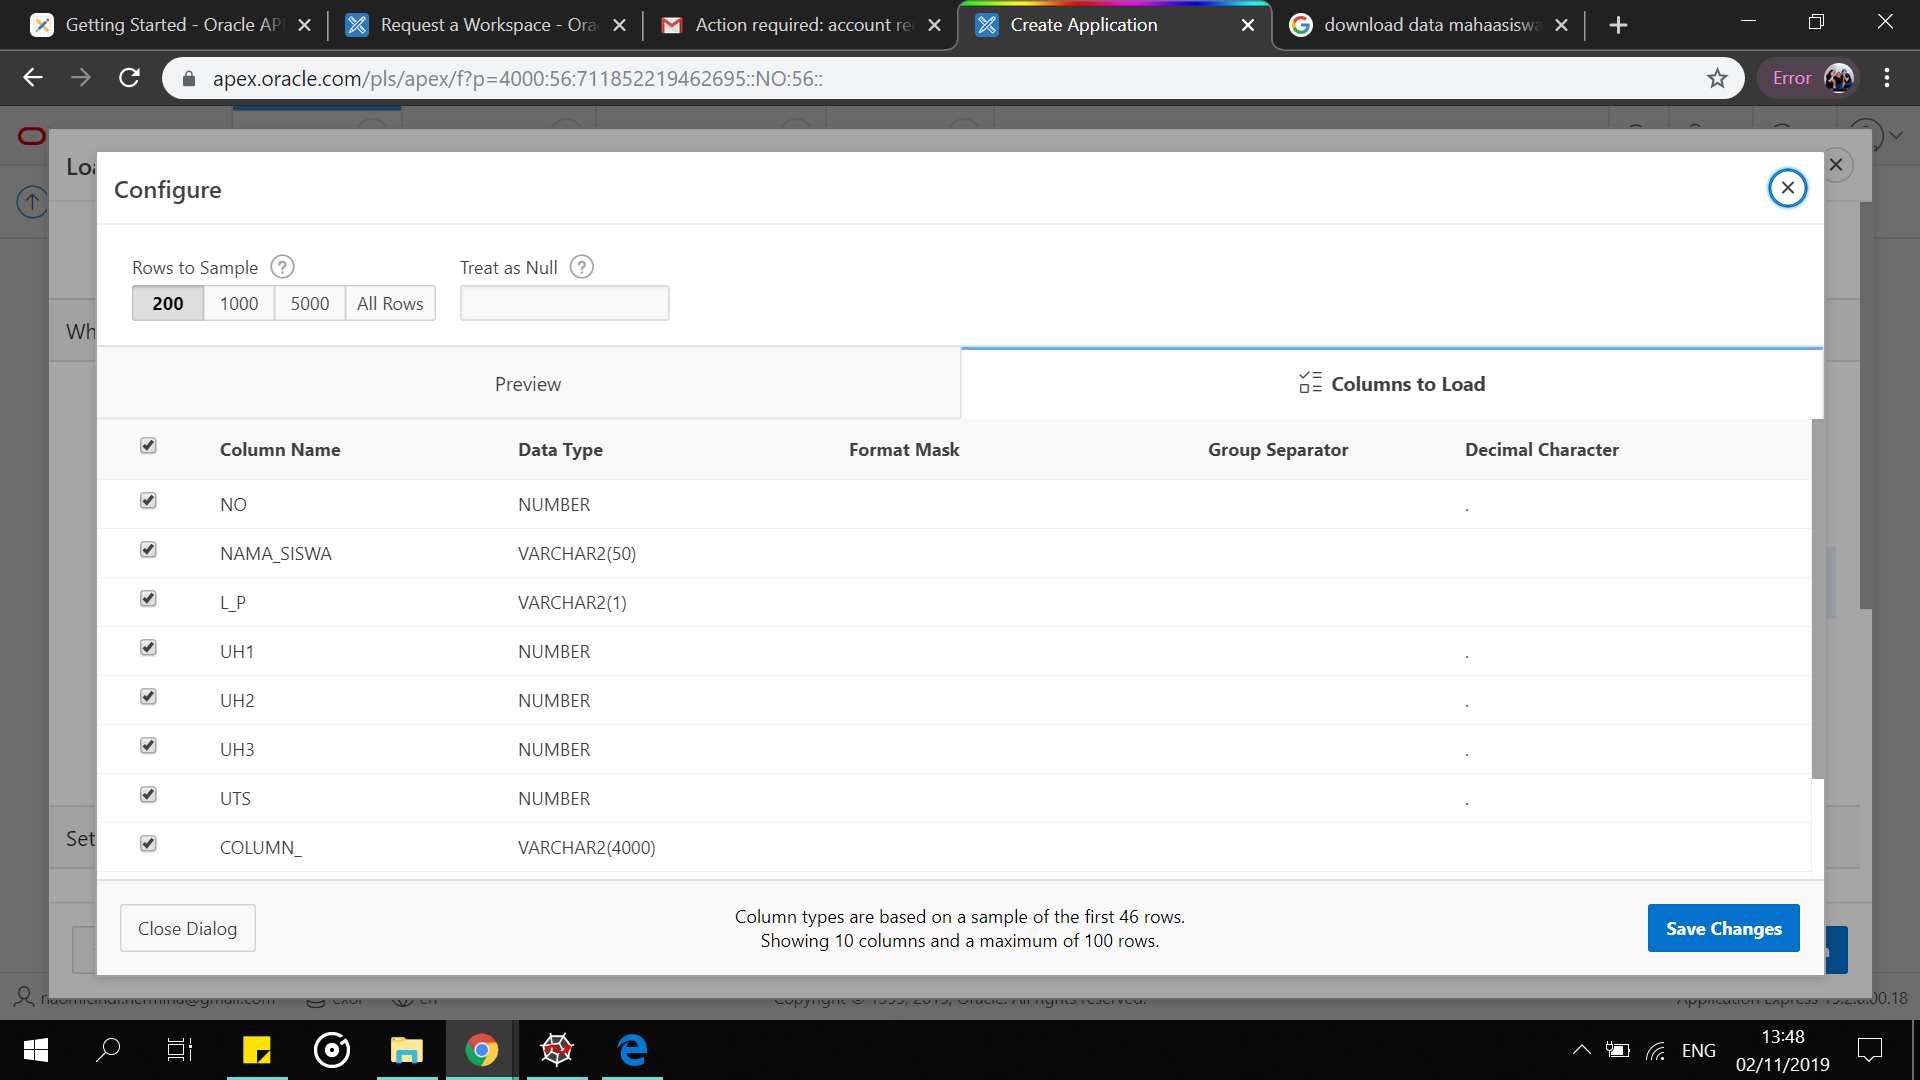
\includegraphics[width=8cm]{picture/23.png}
    \caption{Contoh Column pada Configure}
    \end{figure}
    
\newpage    
\item Tampilan tabel yang sudah di Upload.
\begin{figure}[!htbp]
    \centering
    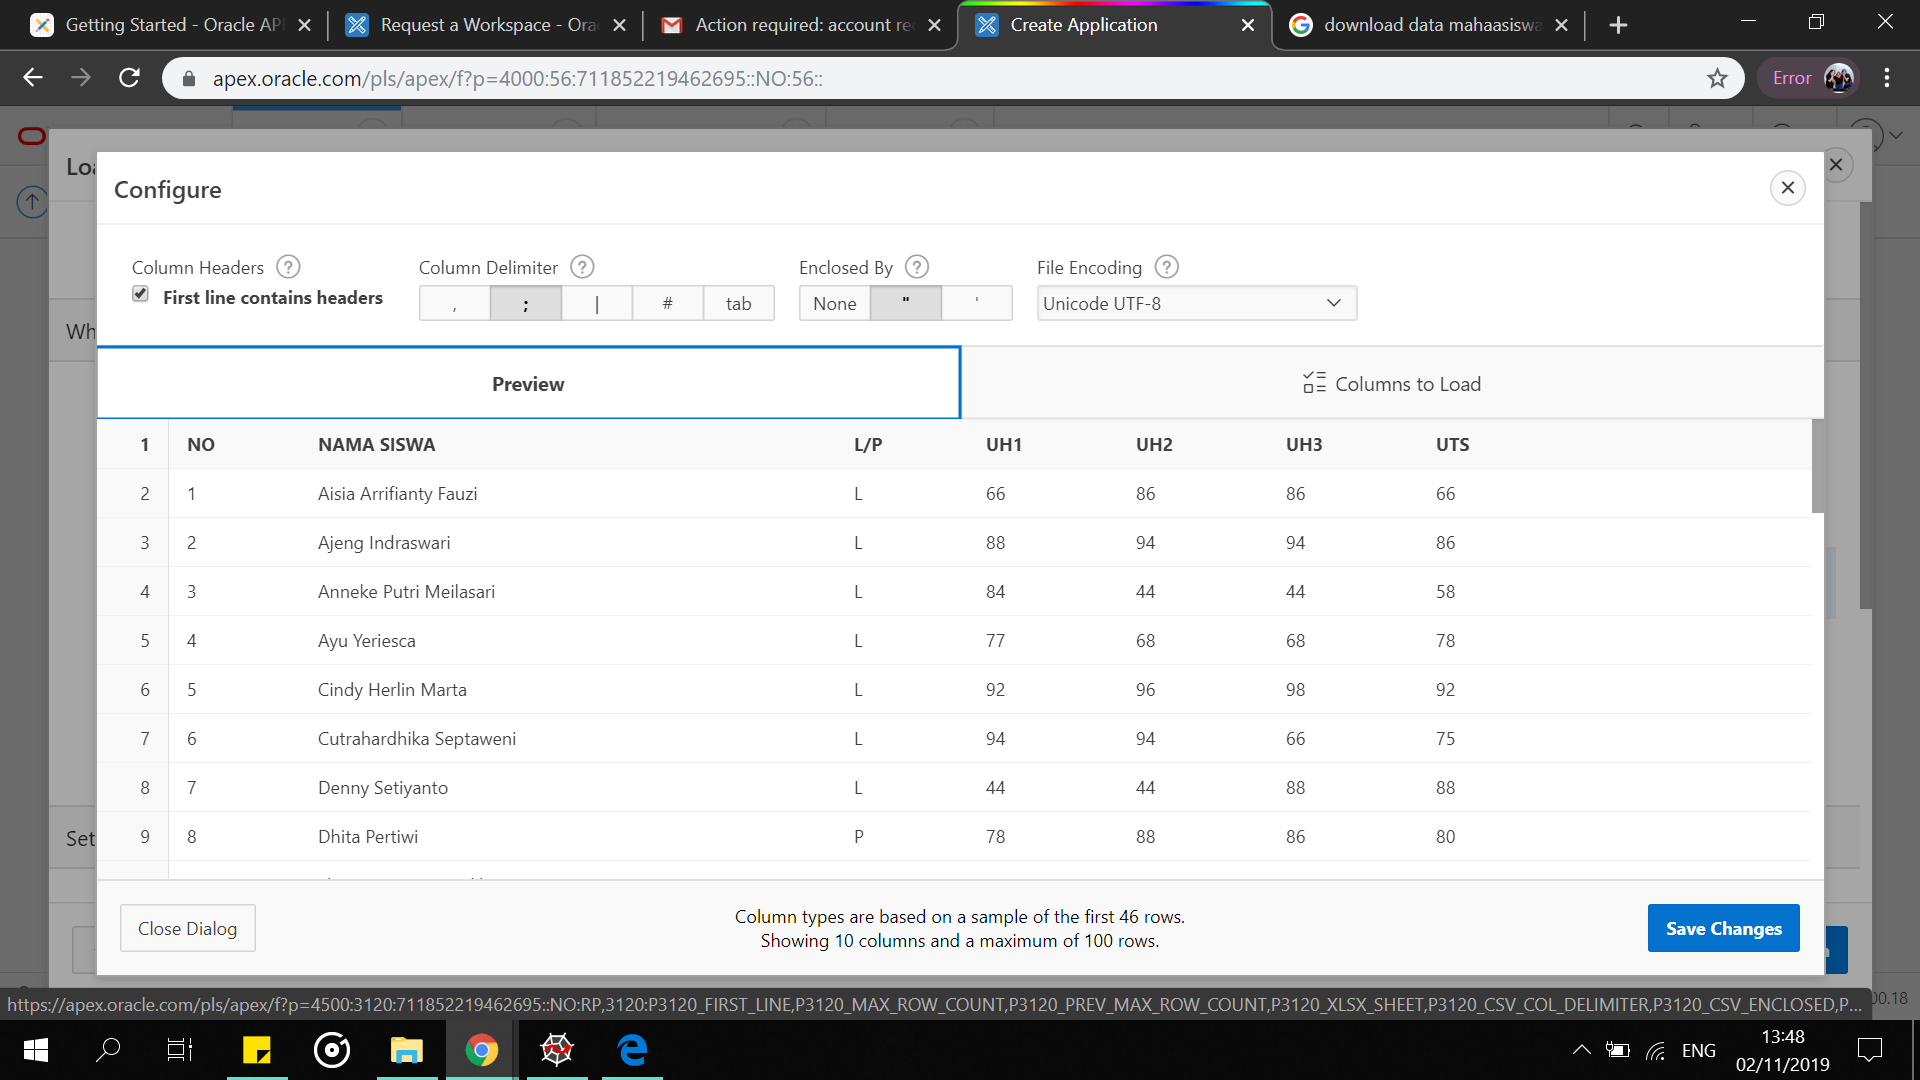
\includegraphics[width=9cm]{picture/24.png}
    \caption{Contoh Priview pada Configure}
    \end{figure}
    
\item Kemudian klik "Save Changes" untuk menyimpan data.
    \begin{figure}[!htbp]
    \centering
    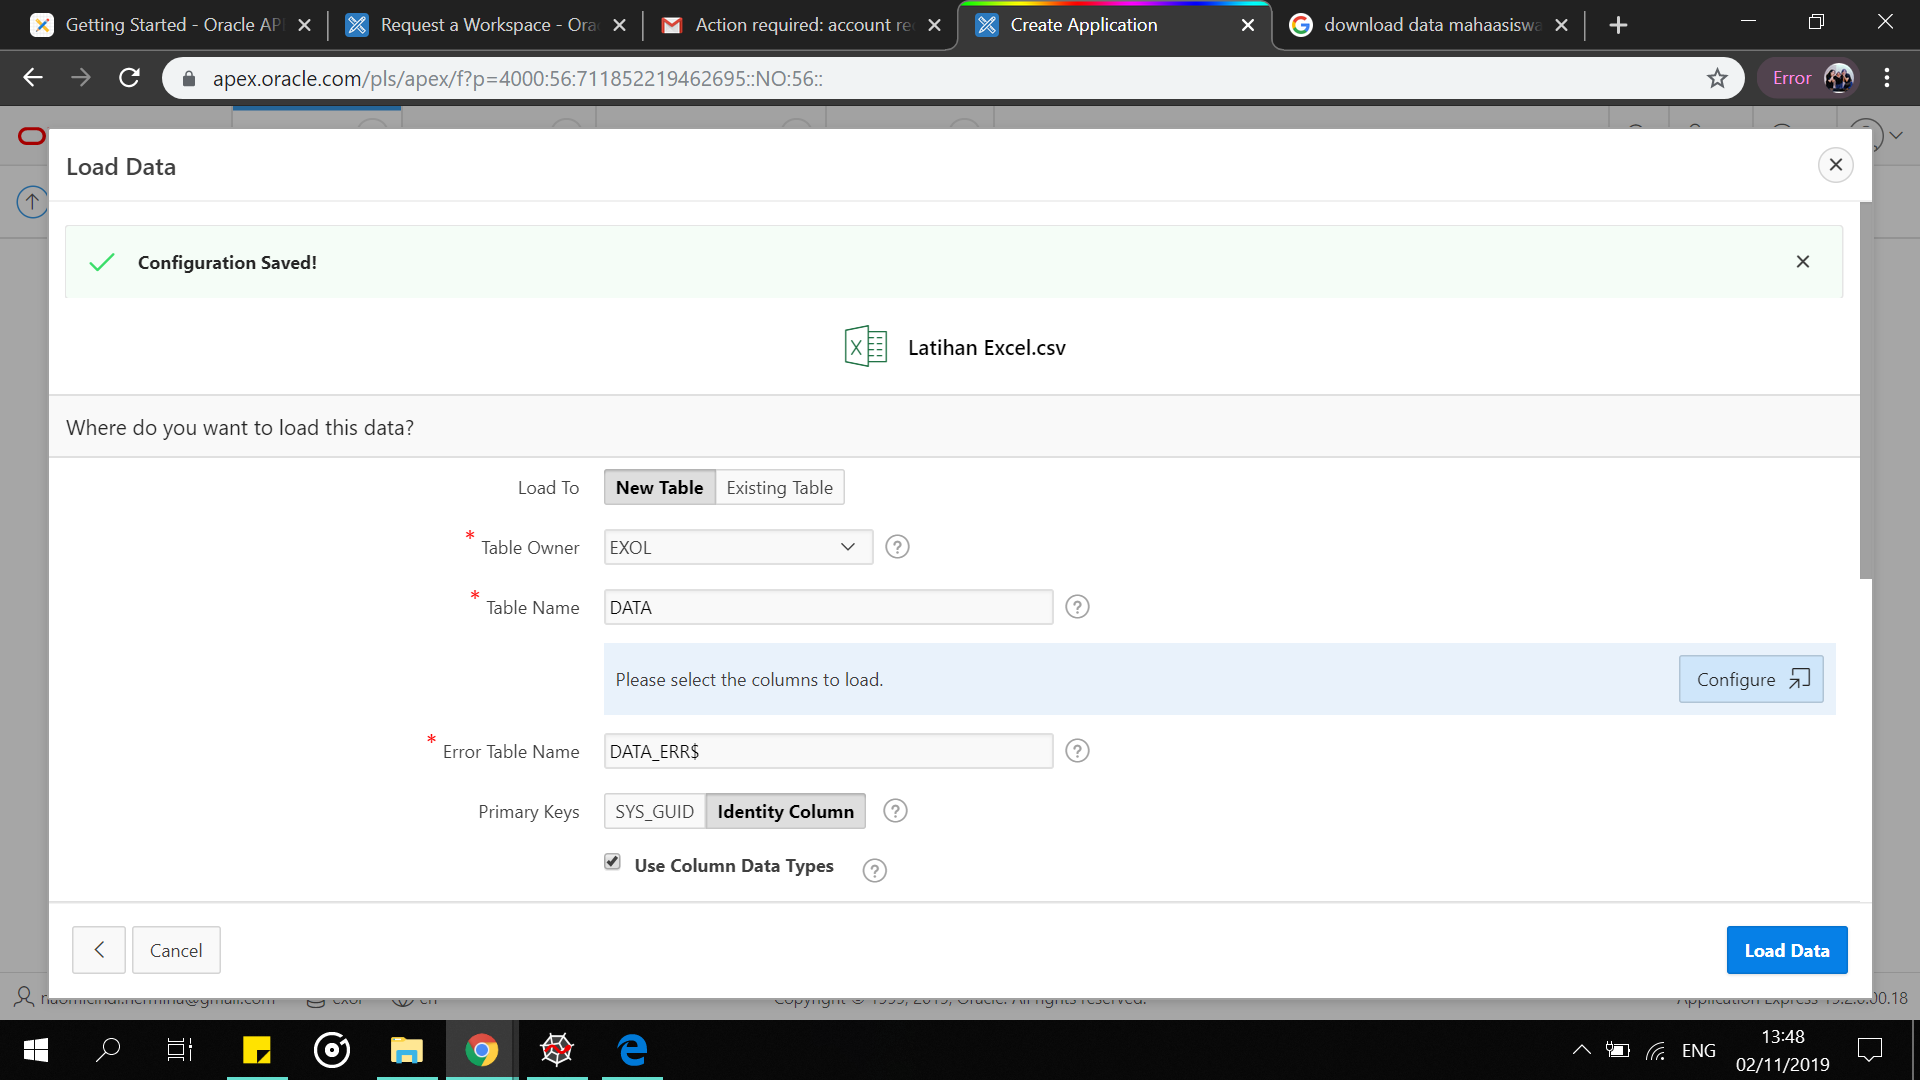
\includegraphics[width=9cm]{picture/25.png}
    \caption{Contoh Menyimpan data}
    \end{figure}
    
\item Tampilan jika tabel berhasil di upload. Kemudian klik "Create Application".
    \begin{figure}[!htbp]
    \centering
    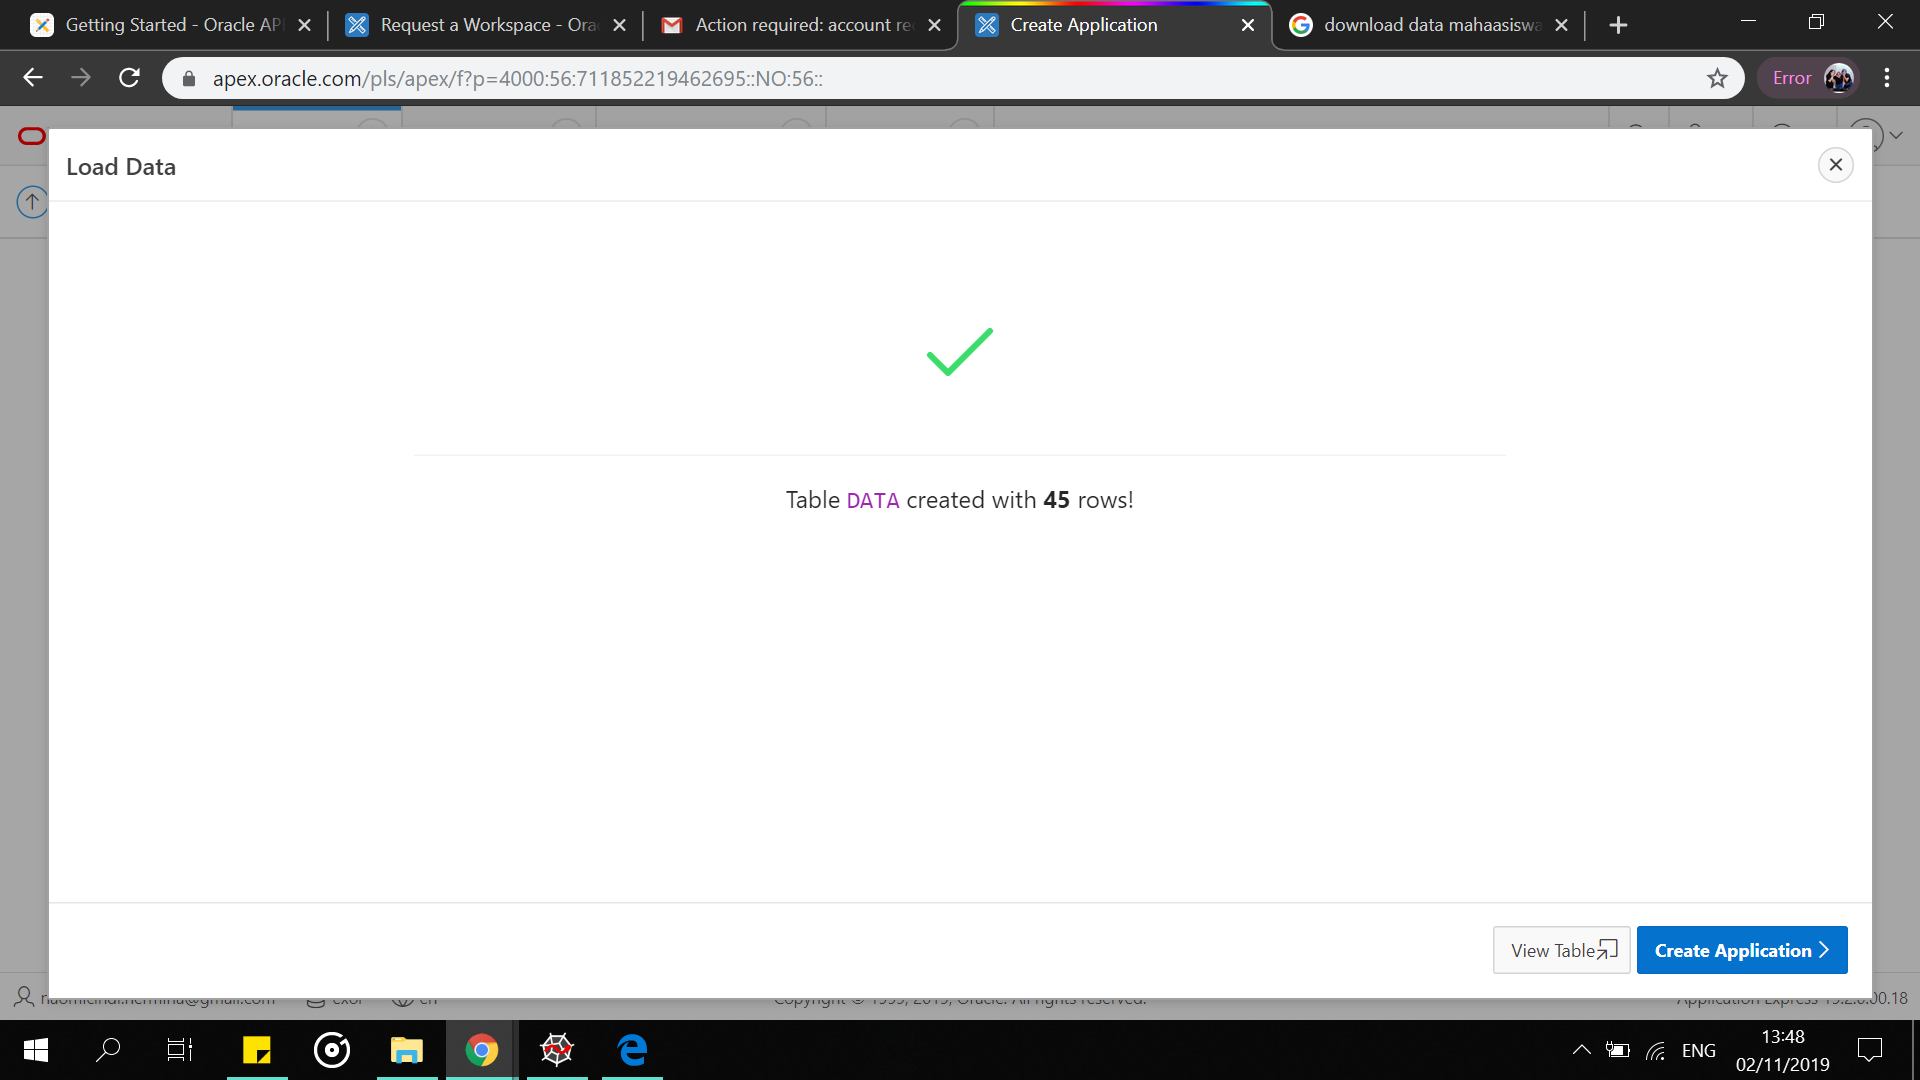
\includegraphics[width=9cm]{picture/26.png}
    \caption{Contoh Tampilan membuat Application}
    \end{figure}
    
\newpage
\item Kemudian samakan nama Tabel yang sebelumnya dengan tabel yang akan dibuat.
    \begin{figure}[!htbp]
    \centering
    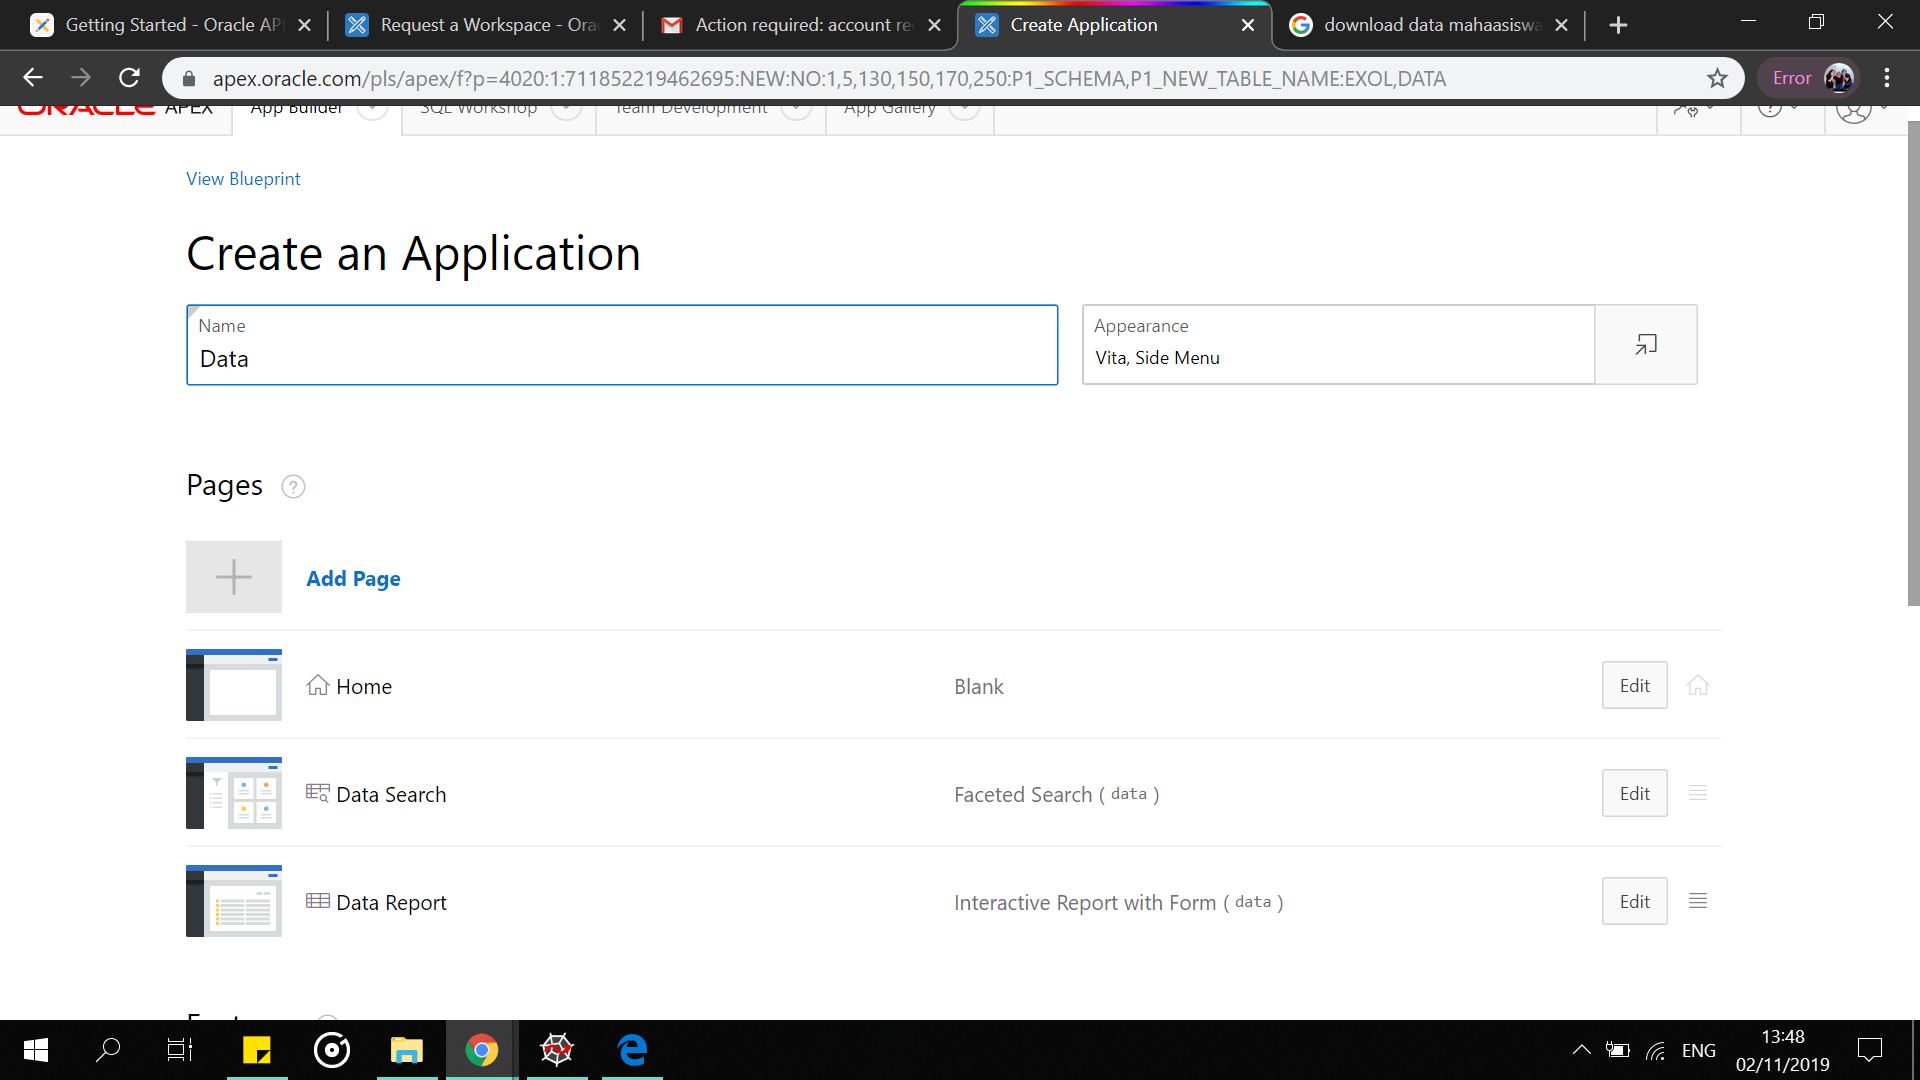
\includegraphics[width=8cm]{picture/27.png}
    \caption{Contoh Membuat nama tabel}
    \end{figure}
    
\item Klik "Create Application" untuk membuat aplikasi apex.
    \begin{figure}[!htbp]
    \centering
    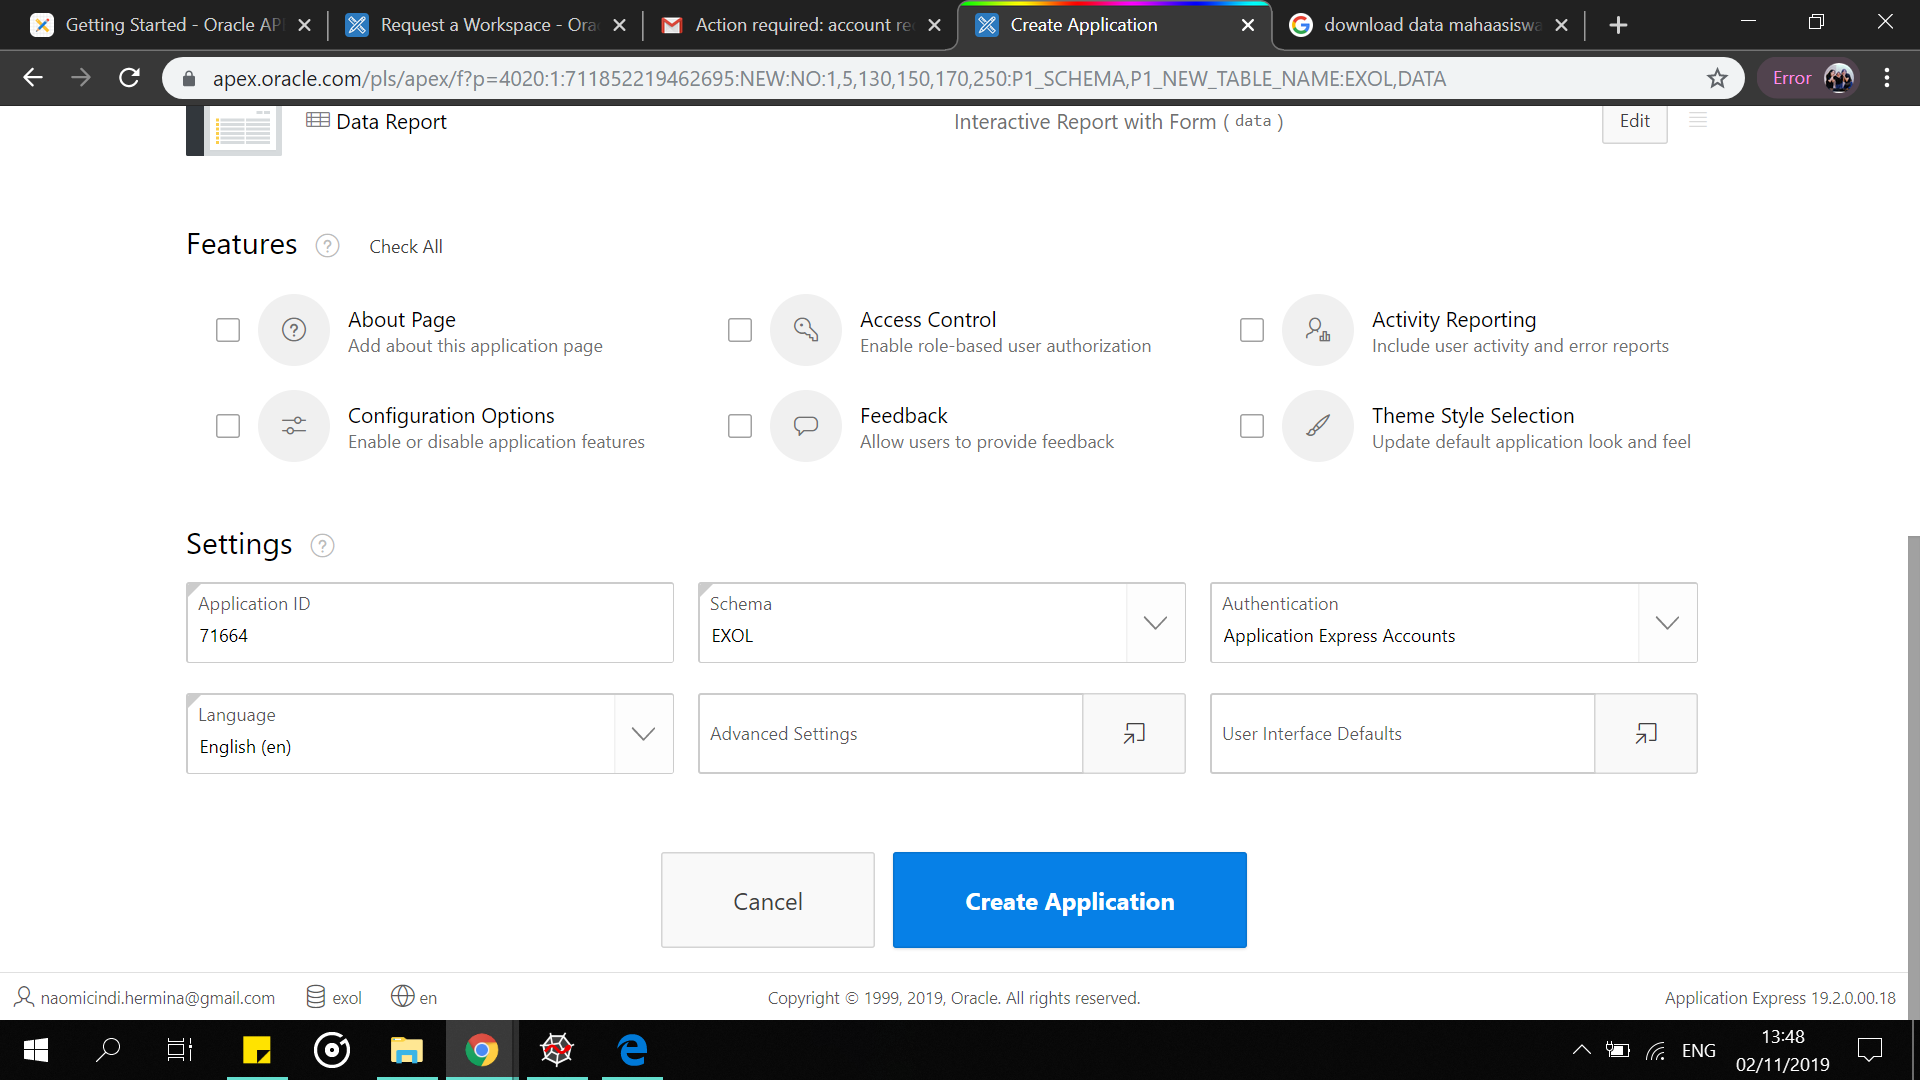
\includegraphics[width=8cm]{picture/28.png}
    \caption{Contoh Membuat Application}
    \end{figure}
    
\item Tunggu sampai aplikasi muncul.
    \begin{figure}[!htbp]
    \centering
    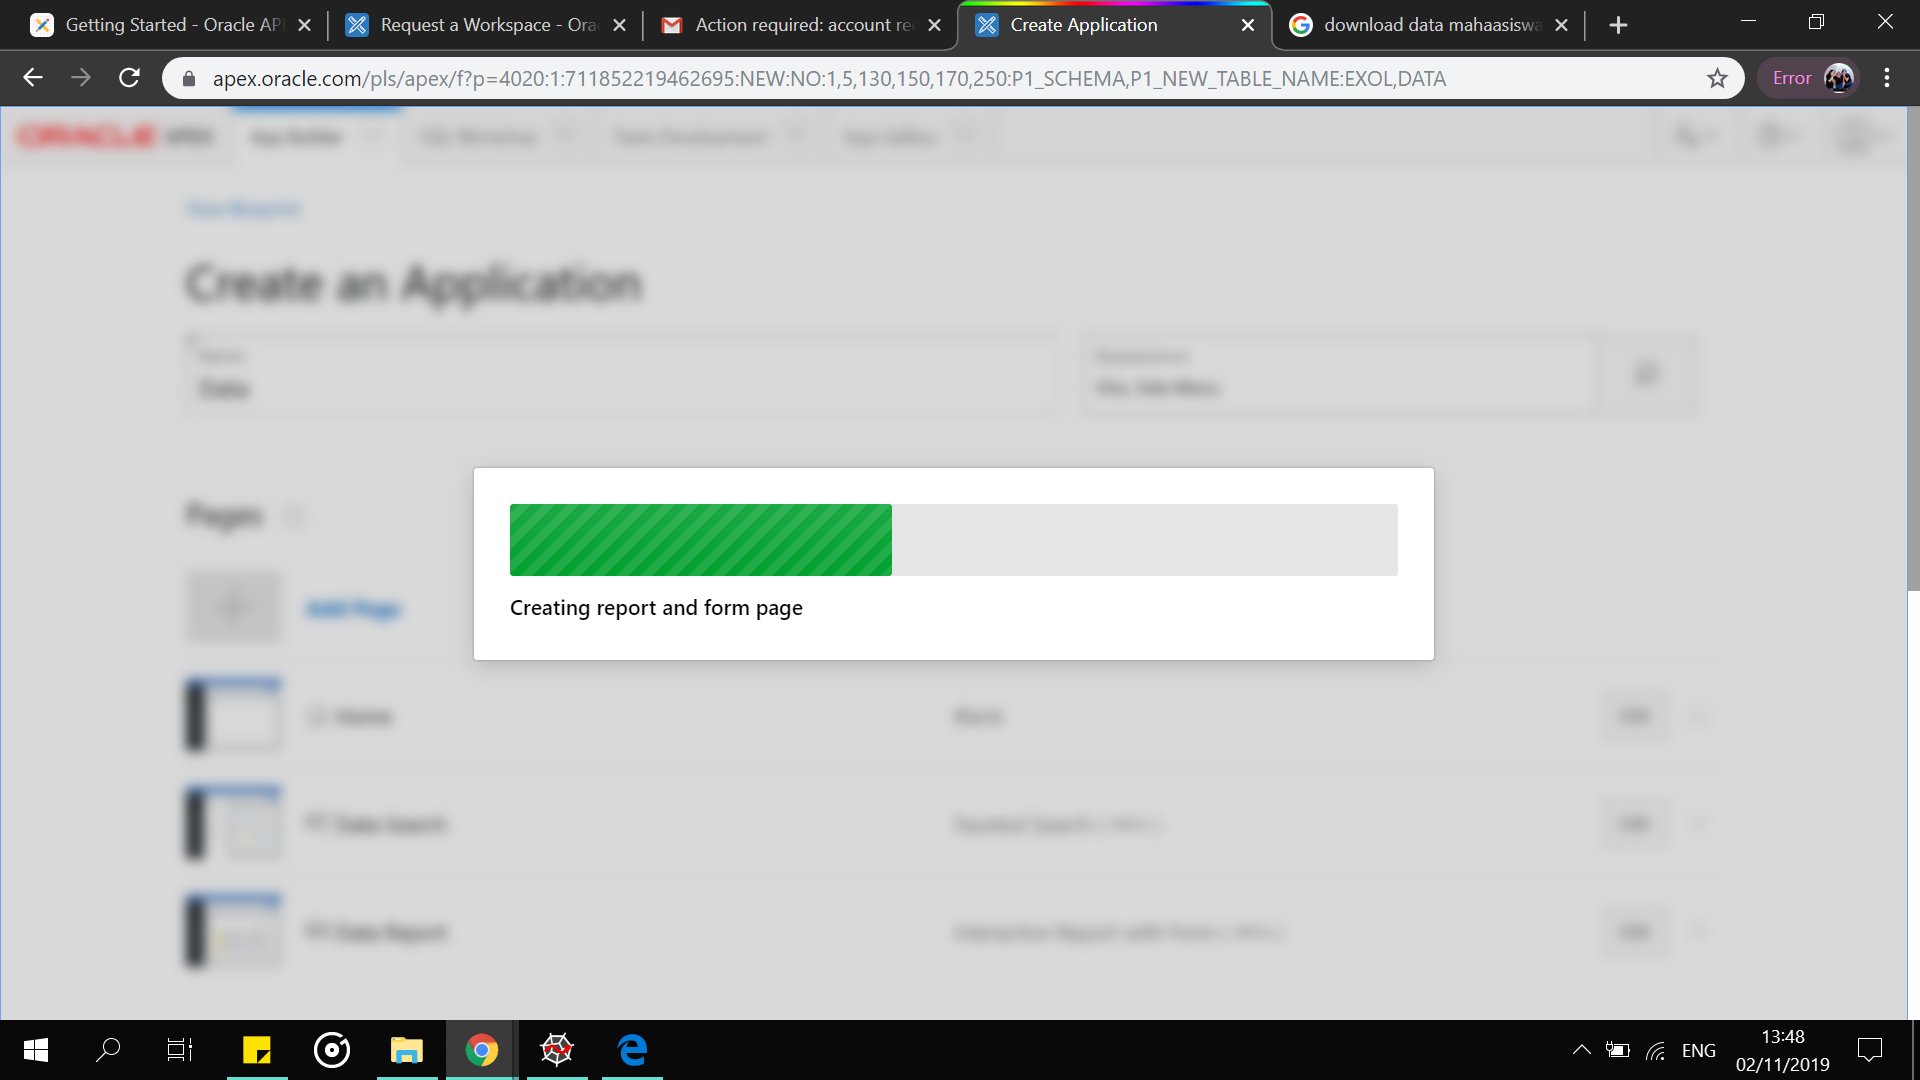
\includegraphics[width=8cm]{picture/29.png}
    \caption{Contoh Proses pembuatan Aplikasi}
    \end{figure}
    
\newpage
\item Kemudian jalankan aplikasinya, caranya klik "Run Application" 
    \begin{figure}[!htbp]
    \centering
    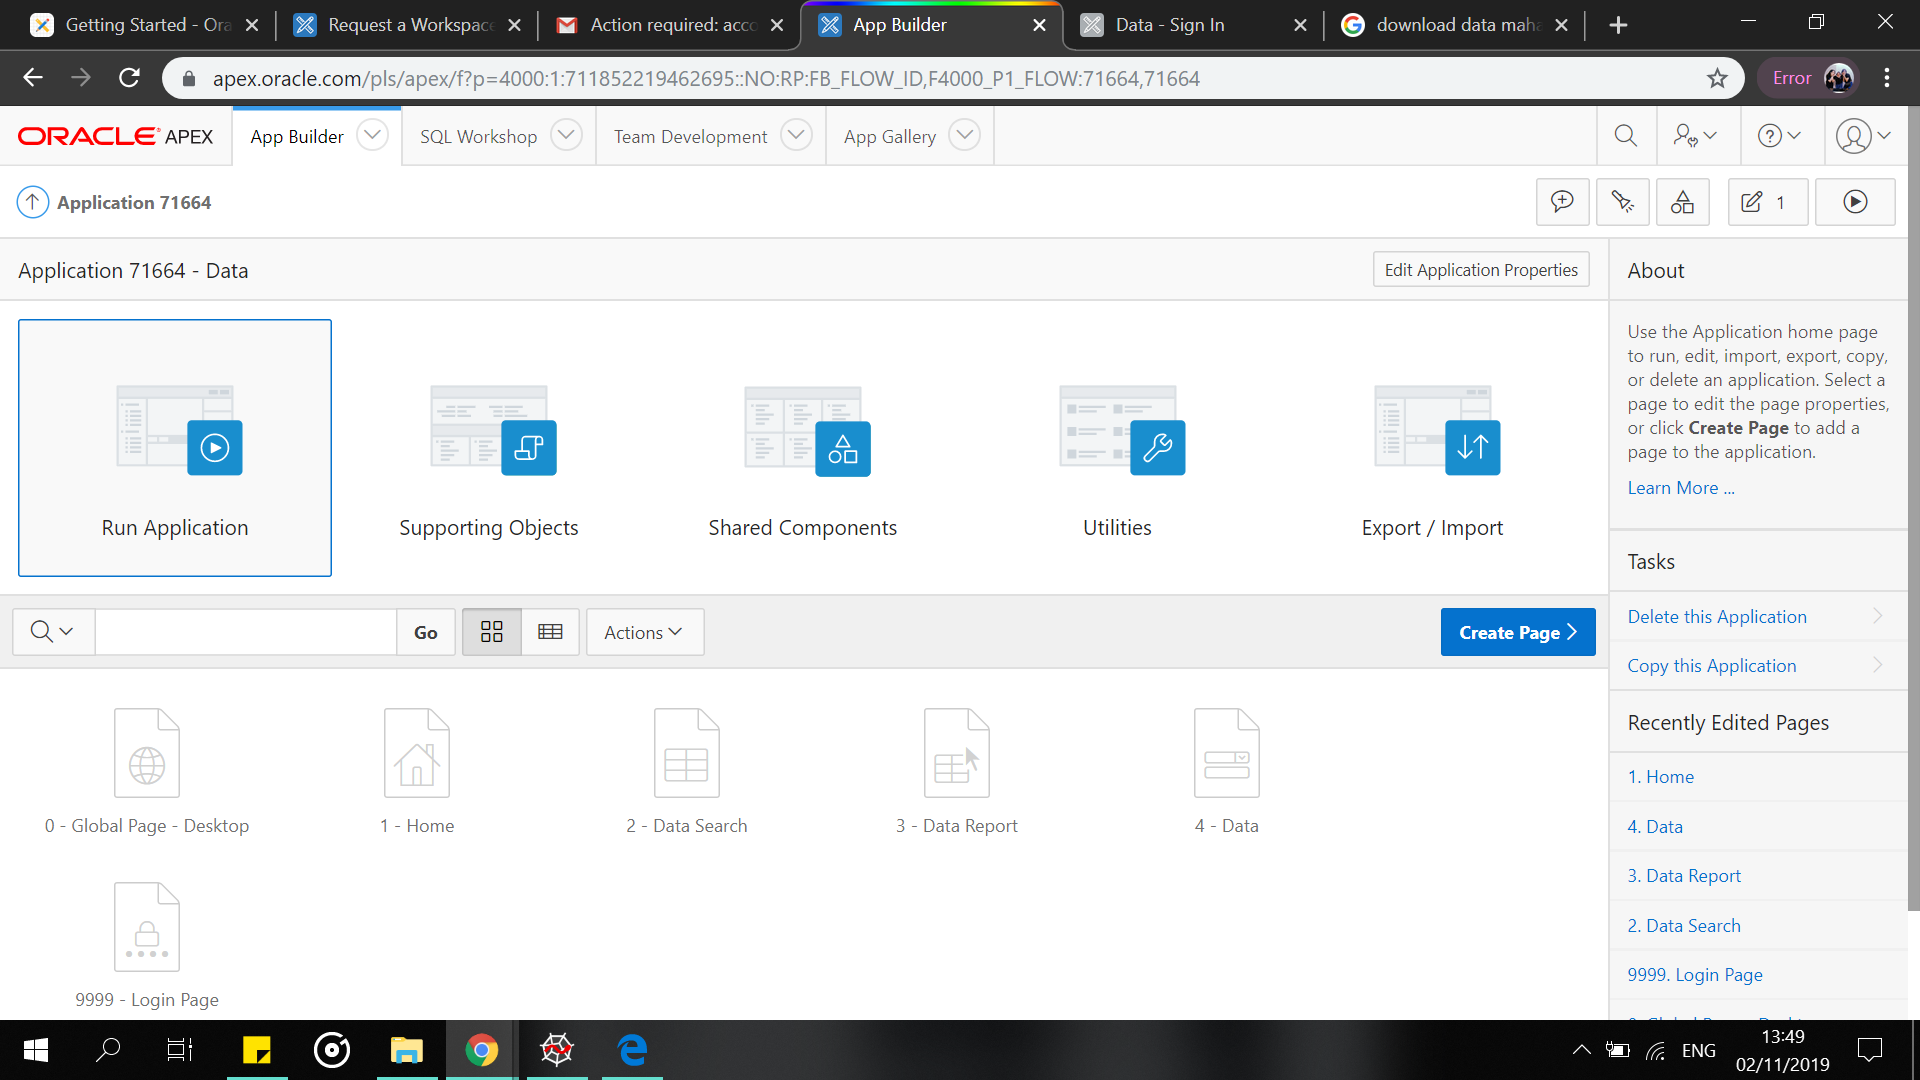
\includegraphics[width=8cm]{picture/30.png}
    \caption{Contoh Menjalankan Aplikasi}
    \end{figure}

\item Masukkan email dan password yang kita daftarkan untuk oracle apex.
    \begin{figure}[!htbp]
    \centering
    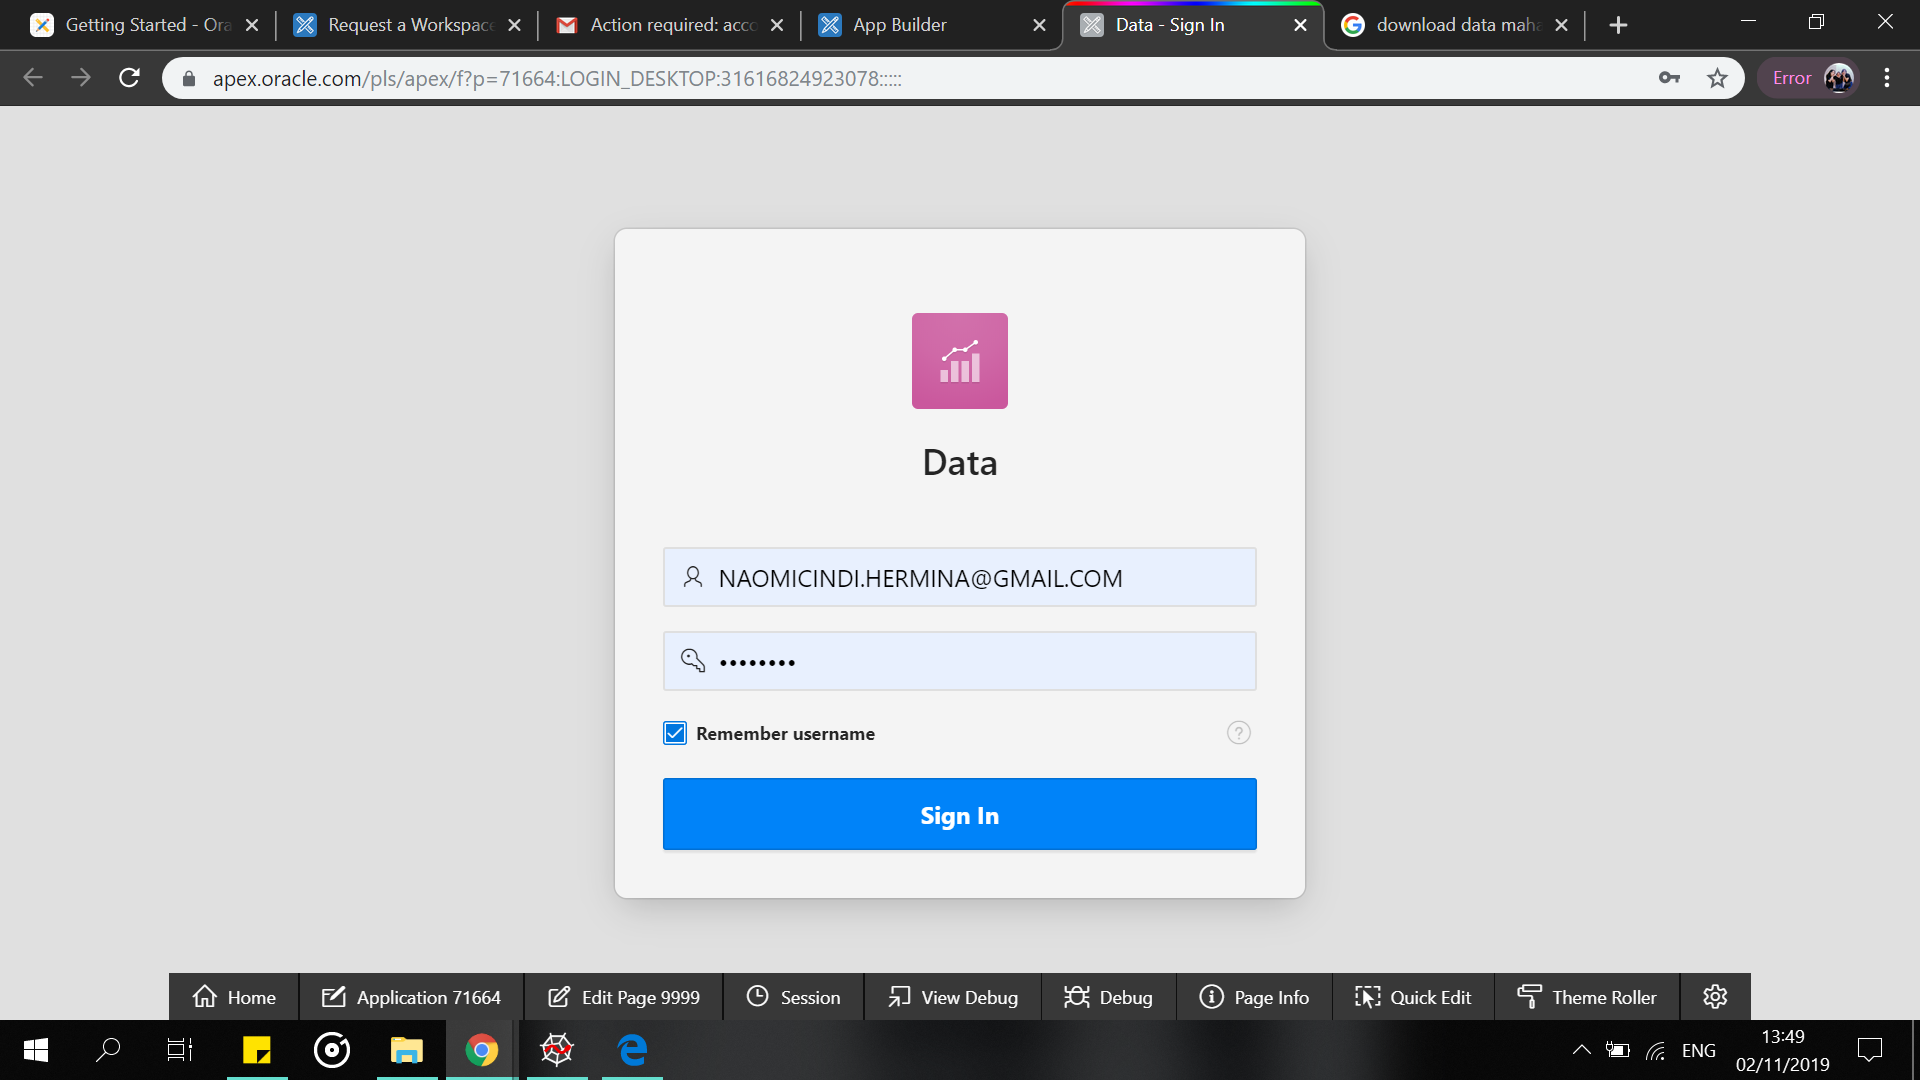
\includegraphics[width=8cm]{picture/31.png}
    \caption{Contoh Sign In pada Application}
    \end{figure}
    
\item Tampilan Application yang digunakan untuk melihat data yang telah di buat, Data Search untuk mensortir data yang ingin kita cari.
    \begin{figure}[!htbp]
    \centering
    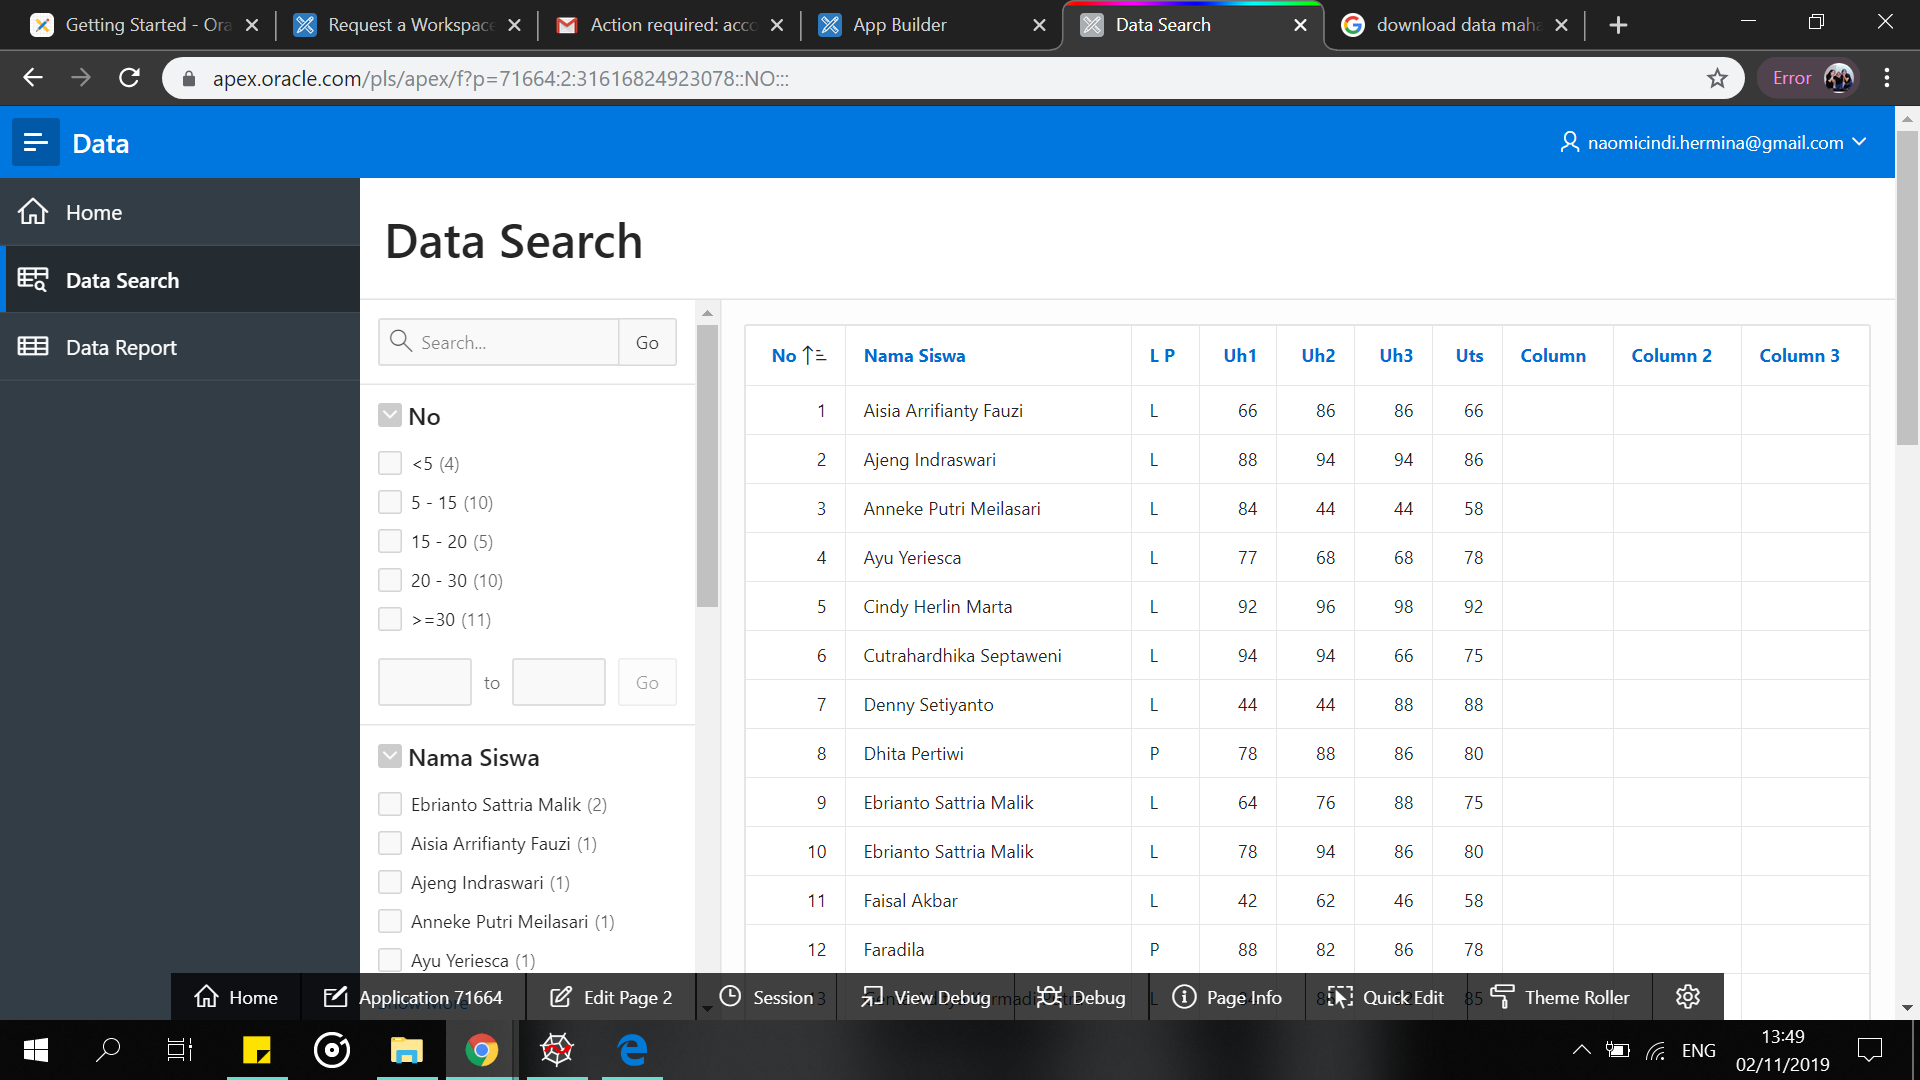
\includegraphics[width=8cm]{picture/32.png}
    \caption{Contoh Tampilan Data pada Applicatio}
    \end{figure}
    
\newpage
\item Tampilan Application yang digunakan untuk melihat data yang telah di buat, Data Report untuk melihat semua Tampilan data.
\begin{figure}[!htbp]
    \centering
    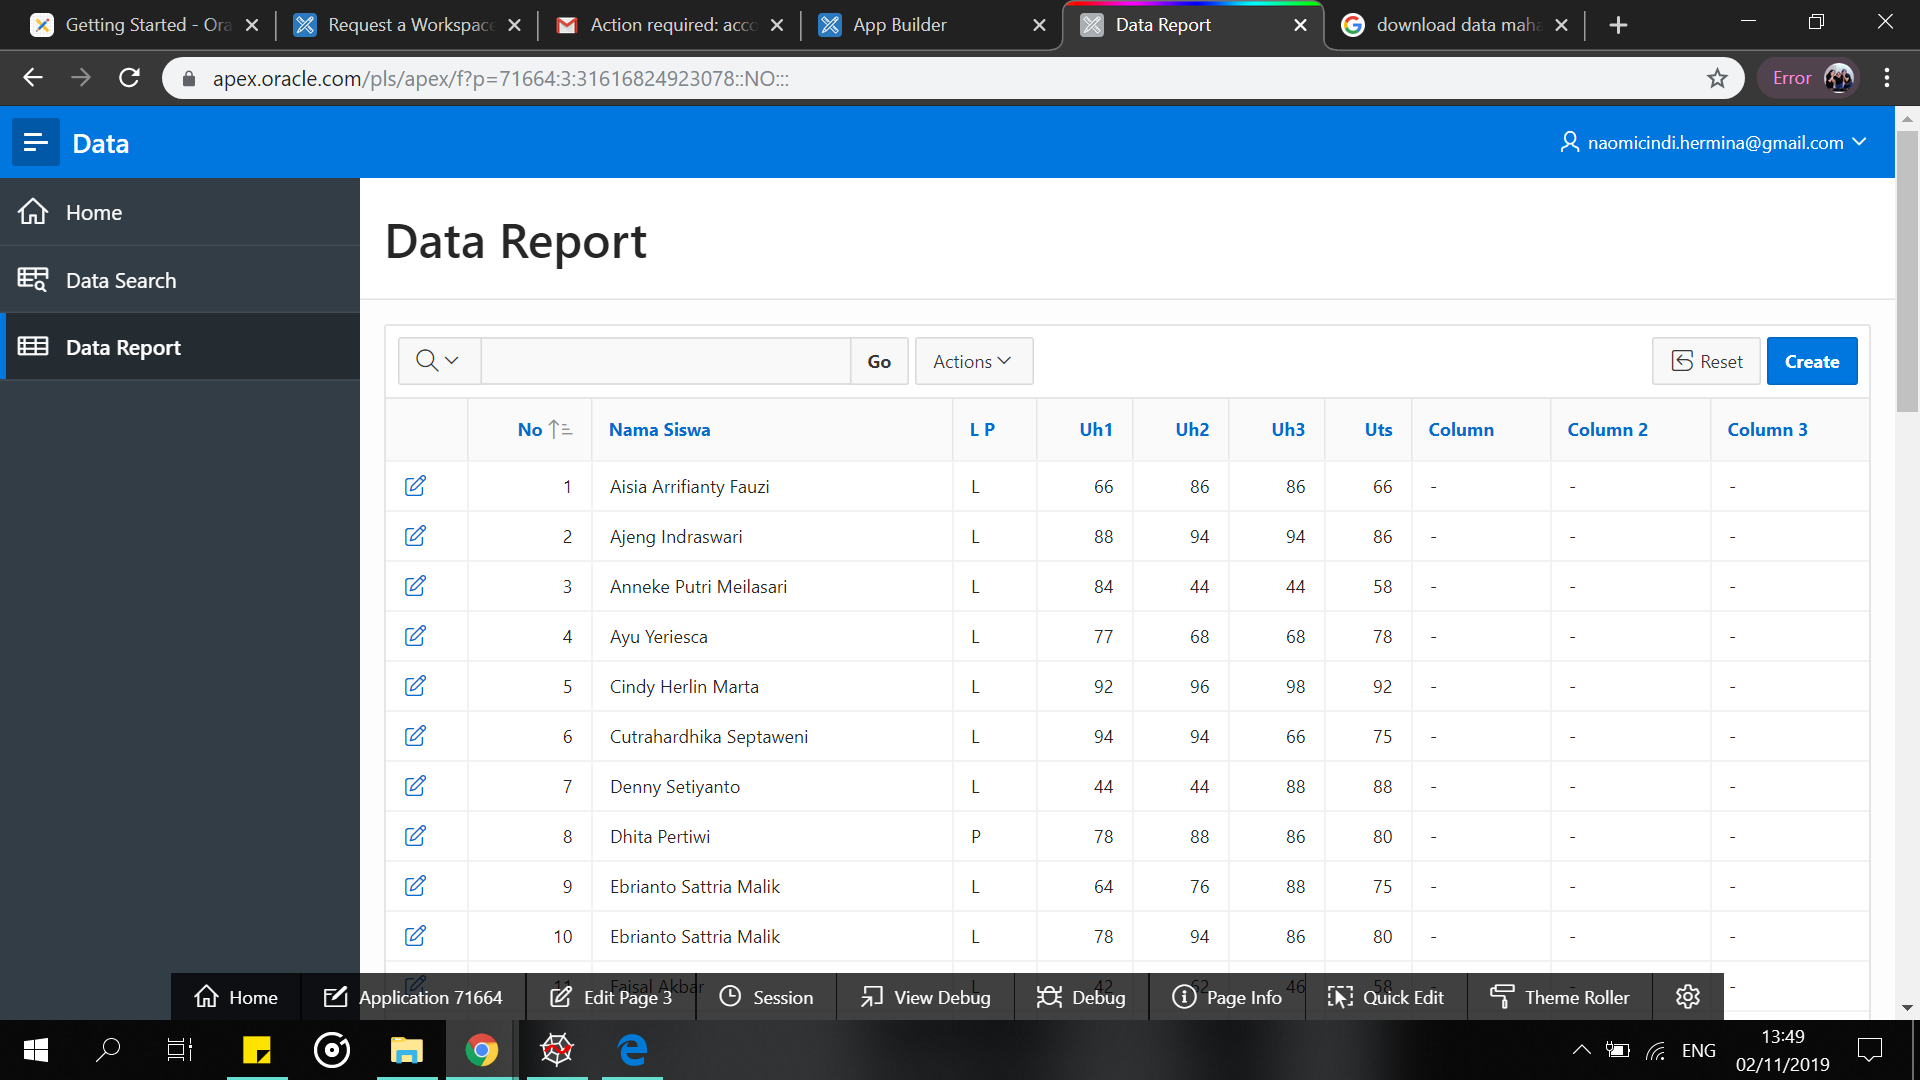
\includegraphics[width=8cm]{picture/33.png}
    \caption{Contoh Tampilan Data pada Application}
    \end{figure}
    
\item Tampilan tabel Data pada Oracle Apex.
    \begin{figure}[!htbp]
    \centering
    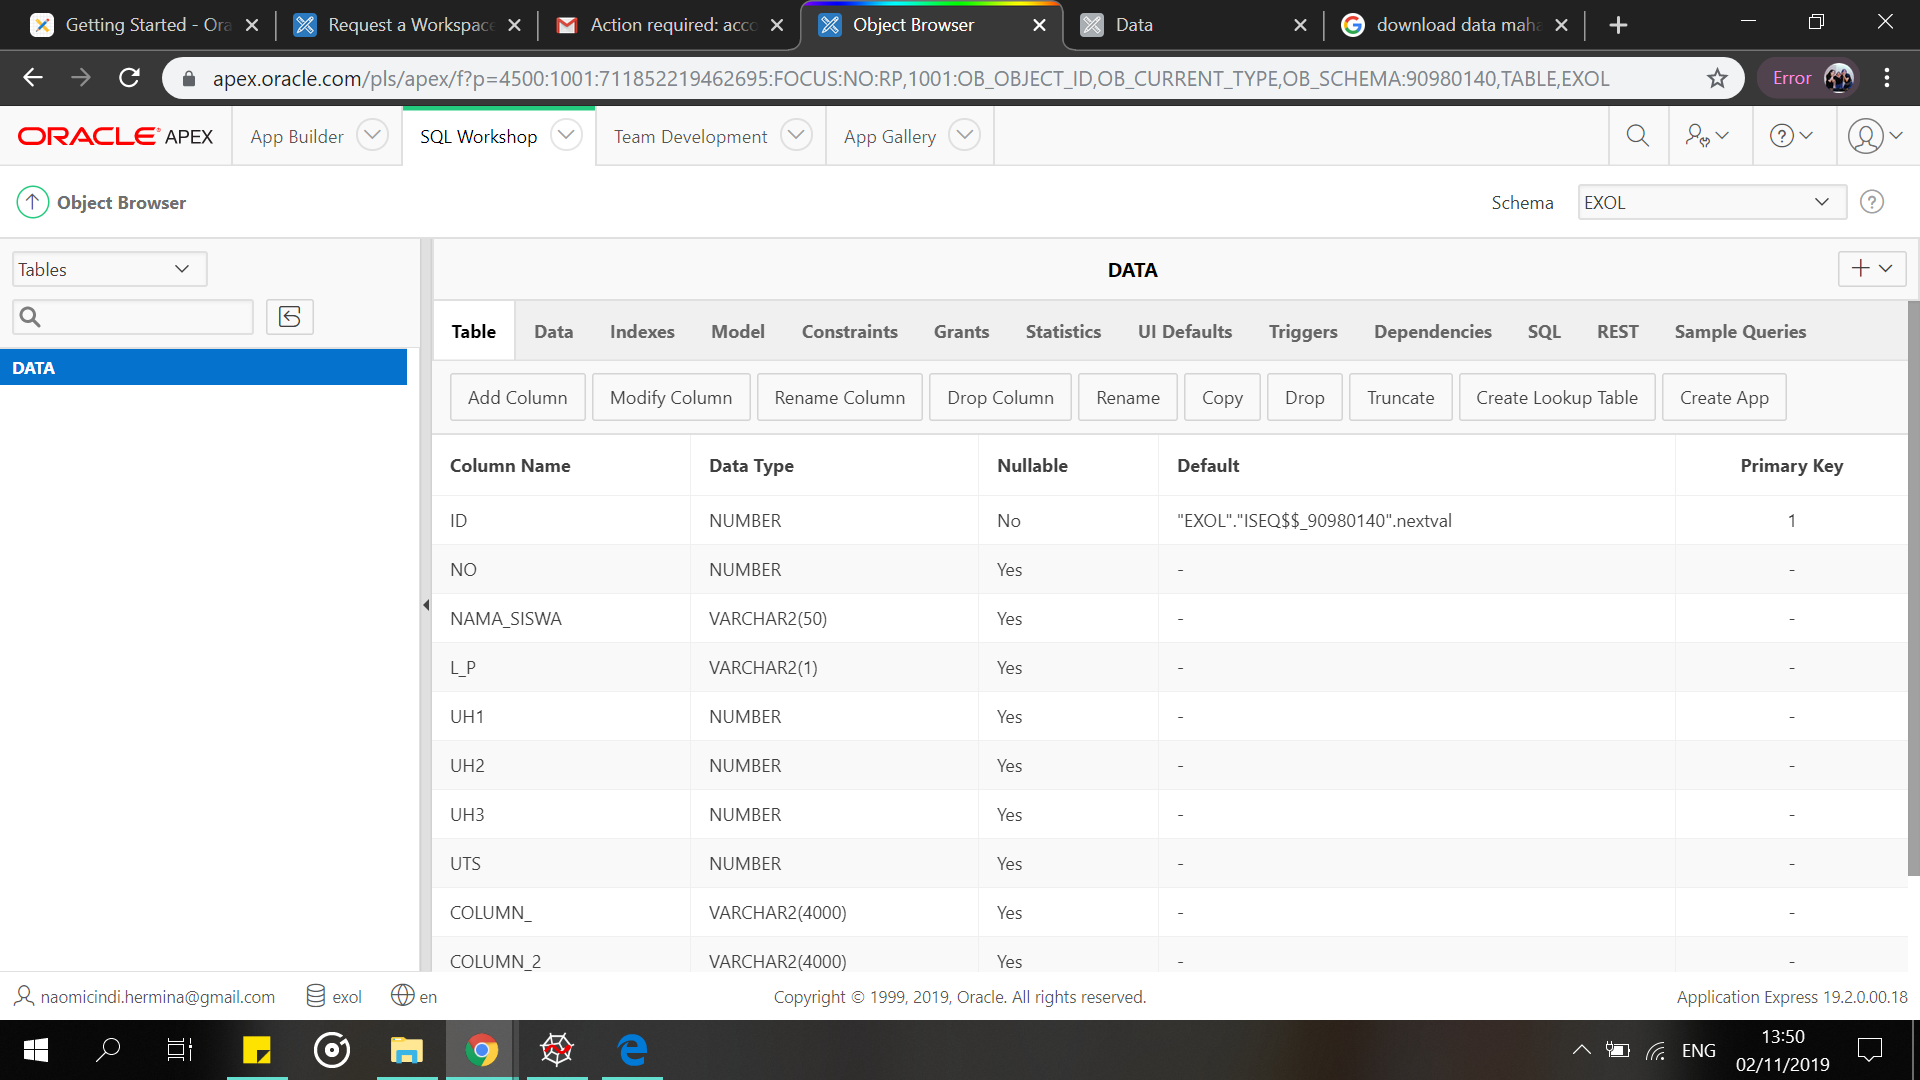
\includegraphics[width=8cm]{picture/34.png}
    \caption{Contoh Tampilan data pada Oracle Apex}
    \end{figure}
    
\item Tampilan tabel Data pada Oracle Apex melalui SQL Workshop lalu pilih SQL Command.
    \begin{figure}[!htbp]
    \centering
    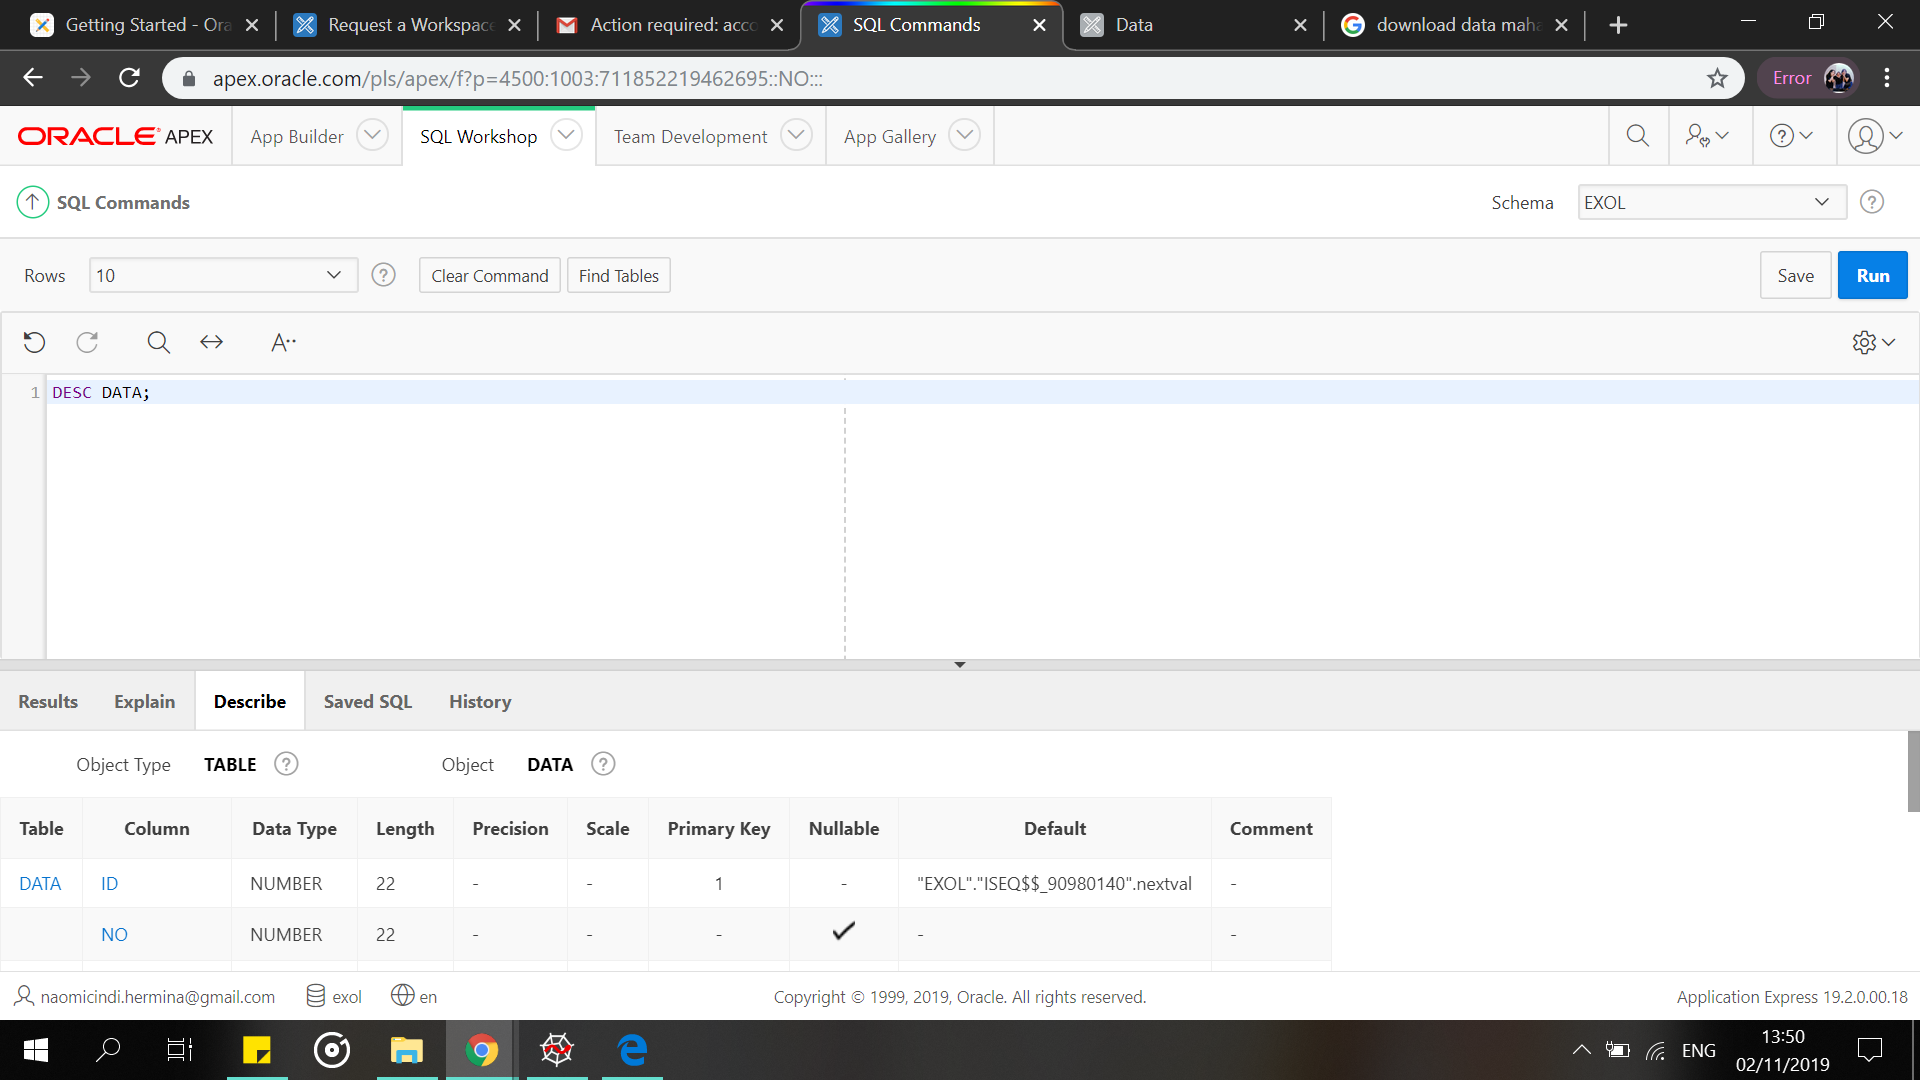
\includegraphics[width=8cm]{picture/35.png}
    \caption{Contoh Tampilan data pada Oracle Apex}
    \end{figure}


    
    
\end{enumerate}


